\documentclass[12pt,oneside]{book}

\usepackage[utf8]{inputenc}
\usepackage[T1]{fontenc}
\usepackage{lmodern}
\usepackage[parfill]{parskip}
\usepackage{amsmath,amssymb}
\usepackage{booktabs}
\usepackage{graphicx}
\usepackage{caption,subcaption}
\usepackage{setspace}

\DeclareUnicodeCharacter{0394}{\ensuremath{\Delta}}
\DeclareUnicodeCharacter{039B}{\ensuremath{\Lambda}}
\DeclareUnicodeCharacter{03A9}{\ensuremath{\Omega}}
\DeclareUnicodeCharacter{2212}{\ensuremath{-}}

\usepackage[backend=biber, bibencoding=utf8, sorting=none]{biblatex}
\addbibresource{refsdm.bib}
\addbibresource{refssidm.bib}
\addbibresource{refssgr.bib}
\addbibresource{refssetup.bib}
\addbibresource{refssims.bib}

\usepackage{hyperref}

\title{Effects of dark matter self-interaction on the evolution of the Sagittarius stream}
\author{Connor Hainje\\\textit{Advised by} Professor Mariangela Lisanti}
\date{April 30, 2021}

\begin{document}

\maketitle

\onehalfspacing
\pagenumbering{roman}

\chapter*{Abstract}

I present a novel test of self-interacting dark matter (SIDM) models by
analyzing the impact of self-interaction on the infall of the Sagittarius
(Sgr) dwarf spheroidal galaxy.  A review of the history of dark matter
detections and the development of the $\Lambda$CDM cosmological model is
included, followed by a review of the motivations for and viability of SIDM
models. Sgr is then presented as a testbed for these models, since its unique
orbital history is highly sensitive to the microphysics determining the Galactic
gravitational potential. I present three simulations of the Sgr infall: two
using collisionless dark matter with cuspy and cored initial galactic profiles,
and one using self-interacting dark matter.  It is found that the inclusion of
dark matter self-interaction has profound impacts on the resulting shape and
distribution of the Sgr stream.  In particular, we find that the distribution of
radial velocities is impacted substantially, with the SIDM merger unable to
reconcile both the shape of the stream and the observed radial velocity of the
progenitor. 

\vspace{0.25in}
This paper represents my own work in accordance with University regulations.

\vspace{0.35in}
\hspace{3.5in}Connor Hainje

\newpage

\chapter*{Acknowledgements}

First and foremost, I would like to thank my advisor, Professor Mariangela
Lisanti, for a fantastic and fulfilling year of research...

I would also like to thank the friends I have made at Princeton...

I would lastly like to thank my family...

\newpage

\singlespacing
\tableofcontents 
\newpage

\pagenumbering{arabic}
\onehalfspacing

\hypertarget{lambda-cdm}{%
\chapter{Introduction}\label{lambda-cdm}}

\hypertarget{evidence-for-dark-matter}{%
\section{Evidence for dark matter}\label{evidence-for-dark-matter}}

In 1932, Jan Oort studied the velocities of stars near the Sun, and he found
that the velocities of these stars were systematically larger than
expected~\cite{oort_force_1932}. From the velocities of stars at a given
radius in a galaxy, one can measure the gravitational mass of all objects
inside that radius. As such, Oort's velocity findings were really a statement
about the mass of the Milky Way. In Oort's own words, these velocities implied
that the amount of gravitating matter in the Milky Way must be larger than
what one can estimate by simply counting stars, with the latter falling short
by roughly 30-50\%~\cite{trimble_existence_1987}.

The next year, Fritz Zwicky studied velocity dispersions in the Coma galaxy
cluster~\cite{zwicky_rotverschiebung_1933,andernach_english_2017}. From his
measurements, he found that the velocity dispersions required ``10 to 100
times more mass'' for the cluster to remain bound than could be accounted for
by luminous matter. He concluded that there must be some large source of
non-luminous matter present to account for the difference, calling the
non-luminous matter ``dunkle Materie'', or ``dark matter''. This is often
cited as the origin of the term.

Over the next few decades, evidence continued to mount for the existence of
dark matter. Rotation curves began being considered, first by Babcock in
1939~\cite{babcock_rotation_1939} and Oort in 1940~\cite{oort_problems_1940}.
In the words of Oort, ``the distribution of mass in this object [the M31
galaxy] appears to bear almost no resemblance to that of light.'' Studies of
globular clusters in the Milky Way indicated that at least two-to-three times
as much mass must lie outside the orbit of the Sun as
inside~\cite{lohmann_masse_1956}.  Studies of binary galaxies revealed large
mass-to-light ratios~\cite{page_average_1960,holmberg_masses_1954}.  More
galaxy clusters were studied, and the trends noted by Zwicky were found to
hold generally~\cite{trimble_history_2013}.  This mounting evidence largely
took the form of acknowledgement of a large mass-to-light ratio; it was not
widely thought that a yet unknown form of matter was responsible.

By the 1970s, however, that would change. This was in large part due to
developments on a few different fronts. First, the 1960s and 70s saw new
methods for measuring the masses of galaxy clusters. Both X-ray measurements
and gravitational lensing first began being used in the 1960s to obtain
measurements of the masses of galaxy clusters~\cite{trimble_history_2013}.
These studies independently confirmed the large, non-luminous masses that were
indicated by the previous velocity analyses.

Second, the cosmic microwave background was discovered in
1965~\cite{penzias_measurement_1965,dicke_cosmic_1965}, and found to be
remarkably isotropic (to better than a part in \(10^4\)).  However, strictly
baryonic models of the universe suggest anisotropies in the CMB on the order
of \(\sim 3 \times 10^{-4}\).  If the Universe contained some non-baryonic
matter which interacted with photons only gravitationally, however, the
predicted anisotropies are revised downward, closer to \(10^{-5}\), consistent
with observation.  Dark matter seems to fit this role perfectly.  Anisotropies
on this scale have been observed by more recent studies, beginning with the
COBE satellite in 1992~\cite{smoot_structure_1992,efstathiou_cobe_1992} and
more recently with the WMAP~\cite{bennett_first-year_2003} and
Planck~\cite{planck_collaboration_planck_2011} missions.

Third, data from rotation curves became quite convincing. Rubin and Ford
published improved optical data from the galaxy M31, the same galaxy studied
by Oort in 1940~\cite{rubin_rotation_1970}. They found that, to even farther
radii than had been previously considered, the rotation curve did \emph{not}
decrease outside the optically bright region of the galaxy, an even stronger
indicator of the existence of mass not accounted for by luminous matter.
Similarly, Roberts and Rots~\cite{roberts_comparison_1973} and Roberts and
Whitehurst~\cite{roberts_rotation_1975} used measurements of 21cm hydrogen
emissions to draw very similar conclusions.

Lastly, 1974 saw two watershed papers by independent research groups, each
concluding that galaxies have dark halos. Einasto, Kaasik, and Saar wrote
``the mass of galactic coronae halos exceeds the mass of populations of known
stars by one order of magnitude, as do the effective
dimensions''~\cite{einasto_missing_1974}. Similarly, Ostriker, Peebles, and
Yahil wrote ``the very large mass-to-light ratio and the very great extent of
the spiral galaxies can perhaps most plausibly be understood as due to a giant
halo of faint stars''~\cite{ostriker_size_1974}. They also note that the year
prior, Ostriker and Peebles had come to a similar conclusion from
considerations of stability, finding the traditional disk galaxy model to be
unstable without a spherical disk~\cite{ostriker_numerical_1973}.

\hypertarget{lambda-cdm-1}{%
\section{Lambda-CDM}\label{lambda-cdm-1}}

Since these discoveries, it has been widely believed among astronomers and
cosmologists that non-baryonic dark matter exists, that it comprises large,
spherical halos around galaxies, and that it played an integral role in the
formation of the structures we can see today. Evidence has become increasingly
strong with improved measurements of the anisotropy in the CMB (such as the COBE
experiment mentioned above), as well as better measurements of the masses of
various structures thanks to improved rotation curves and better X-ray and
gravitational lensing instrumentation.

Another major question of the twentieth century which came to be largely
settled toward its end was that of the cosmological constant, \(\Lambda\).
This constant was introduced by Einstein into his theory of general relativity
as a means to achieve a static universe, though today it is used to describe the
accelerating expansion of the universe.  Physically, this constant can be
interpreted as the vacuum energy density of empty space.  It is often called
``dark energy'' for this reason~\cite{schneider_extragalactic_2015}.  In the
late 1990s, measurements of Type Ia supernovae strongly constrained
\(\Lambda\) to be positive, giving empty space a significant, constant vacuum
energy~\cite{riess_observational_1998,perlmutter_measurements_1999}.

These findings, combined with large amounts of evidence for the Big Bang
hypothesis, are all most simply described by the \(\Lambda\)CDM model,
sometimes called the standard model of cosmology or the concordance model~\cite{dodelson_modern_2021}. The model describes the Universe as consisting
of three components---the cosmological constant \(\Lambda\), cold dark matter
(CDM), and standard matter---operating under general relativity and coming
from an origination event roughly 14 Gyr ago (the Big Bang). This rather
simple model is remarkably successful at explaining the Universe.

Through its inclusion of the Big Bang event, the \(\Lambda\)CDM model gives an
explanation for the origin of the CMB. In this model, the CMB is a residual
radiation left-over from a period shortly after the Big Bang, where the
Universe was hot (\textgreater{}10,000 K). As the Universe cooled and
structures began to form, the photons from this period began to propagate
freely in all directions.

The \(\Lambda\)CDM model also provides a well-tested account of the formation
of structures in the Universe~\cite{dodelson_modern_2021}. In the early
Universe, small gravitational perturbations caused matter to collapse into
small structures. These small structures---effectively perturbations in
the mass density of the Universe---created gravitational potential wells,
attracting other small structures and assembling together to produce larger
ones. This works especially well for describing the distribution of dark
matter in the Universe, as small pockets of dark matter converge to form
subhalos, halos, and larger. The case for baryonic matter and galaxy formation
is more complicated, involving baryonic processes, gas dynamics, and more, but
is also well-explained in the régime of hierarchical structure formation.
Simulations of hierarchical structure formation have found that it is able to
account well for the observed distribution of structures on the scales of
galaxies, galaxy clusters, and larger. The implications of this model of
structure formation are considered in more detail in the next section.

In fact, the success of this theory of structure formation serves as reason to
believe that dark matter is cold (hence the ``C'' in \(\Lambda\)CDM). Dark
matter being ``cold'' means that it was non-relativistic at the time of
decoupling (the period in the early Universe when matter began to fall out of
thermal equilibrium)~\cite{mohanty_astroparticle_2020}. By contrast, ``hot'' dark matter
(HDM) would have been relativistic at the time of decoupling. Given these
higher velocities, the velocity dispersion of HDM would have been
non-negligible (differing from the negligible velocity dispersion of CDM). A
finite velocity dispersion, however, would have prevented the dark matter
particles from being bound to shallow gravitational potential wells, further
preventing the formation of small-scale
structures~\cite{schneider_extragalactic_2015}. Thus, HDM fails to form
structure.

On its own, \(\Lambda\)CDM is remarkably able to explain most of our
observations of the Universe. However, there are a few cosmological problems
which have arisen. One is known as the horizon
problem~\cite{bergstrom_cosmology_2008,schneider_extragalactic_2015}, which
points out the the CMB is, to a high degree, isotropic, indicating that the
photons making up this radiation are roughly in thermal equilibrium across the
sky. However, this means that regions of the sky which are too far separated
to be causally connected have remained in equilibrium. This is not explained
by \(\Lambda\)CDM.

Another problem is the flatness problem, which points out that there is
potentially a fine-tuning problem with the vanilla \(\Lambda\)CDM
model~\cite{bergstrom_cosmology_2008,schneider_extragalactic_2015}. The
Universe as we observe it is approximately flat today, meaning that its
curvature is approximately unity. If the curvature were not unity, its
deviation from flatness is expected to grow with time. As such, if the
Universe is not flat, it must have been \emph{very} close to unity at early
times, meaning that this parameter may need to be ``fine-tuned'' to achieve a
reasonable explanation. The problem is that our model should be able to
describe parameters like these \emph{without} fine-tuning.

Combining the \(\Lambda\)CDM model with the theory of cosmic inflation,
however, solves both of these problems~\cite{bergstrom_cosmology_2008}.
Inflation posits that the Big Bang was followed by a period of rapid
(exponential!) inflationary expansion. Such a phenomenon would solve the
horizon problem, as the whole observable Universe would have originated from a
much smaller, thermally-connected region before inflation. It also solves the
flatness problem, as inflation would have significantly stretched and
flattened any curvature in the Universe, providing a natural explanation for
the observed flatness today. In fact, this creates a sort of inverse
fine-tuning problem: in this theory, any curvature which is \emph{far} from
unity requires fine-tuning.

\hypertarget{structure-formation}{%
\section{Structure formation}\label{structure-formation}}

As stated above, the \(\Lambda\)CDM model predicts structures to form in
the Universe as a result of gravitational perturbations at early times.
As expansion slows, the pockets of matter created by these perturbations
host small gravitational potential wells, causing nearby matter to
collapse inward and the growth of structure to occur. With the majority
of matter in the Universe being dark matter, the first structures which
occur are pockets of dark matter halos. The halos observable today are
the result of the hierarchical combination of smaller halos.

The abundance of these halos can be described by extended
Press-Schechter (EPS) theory~\cite{bullock_small-scale_2017}. This
theory is grounded on rather simple assumptions: that one can use a
spherical collapse model and that one can extrapolate from linear
perturbation theory even into non-linear régimes. Despite these
assumptions, it has been shown to give predictions about the mass
spectrum of dark matter halos which are in accord with high-resolution
numerical simulations.

The halos themselves can be described as virialized objects with mass
\begin{equation}
M_{\text{vir}} = \frac{4\pi}{3} R_{\text{vir}}^3 \Delta_c \rho_c,
\end{equation}
where \(R_{\text{vir}}\) is the virial radius, \(\rho_c\) is the
critical density of the Universe, and \(\Delta_c\) is the over-density
parameter. As noted in~\cite{bullock_small-scale_2017}, identifying the mass of
a halo requires a way of defining the outer edge, or the radius, of the halo,
and this is done by a choice of $\Delta_c$. It is often chosen to match the
expected over-density for dark matter in a region which undergone an idealized
spherical collapse. Such values are often on the order of $\mathcal{O}(100)$; in
this work, we choose to follow a common convention by setting \(\Delta_c =
200\).  We thus mark the virial mass and radius with a subscript 200 instead
of ``vir''.

The \(\Lambda\)CDM model also provides predictions about the internal
structure of these dark matter halos. Dark matter-only N-body simulations were
performed as early as 1988~\cite{frenk_formation_1988}, with higher-resolution
simulations like~\cite{dubinski_structure_1991}
and~\cite{navarro_structure_1995} following shortly thereafter. The resulting
halos from these simulations were found to agree remarkably well with a
\emph{two-power} density profile~\cite{binney_galactic_2008} 
\begin{equation} \label{eq:twopower}
\rho(r) = \frac{\rho_0}{(r/a)^\alpha (1 + r/a)^{\beta-\alpha}}, 
\end{equation}
where \(\rho_0\) is a characteristic density for the halo and \(a\) is the
length scale. Special cases of this model include \((\alpha,\beta) = (1,4)\),
the Hernquist model~\cite{hernquist_analytical_1990}, and \((\alpha,\beta) =
(1,3)\), the NFW model~\cite{navarro_structure_1995,navarro_universal_1997}.
In general, the NFW model enjoys the most usage as one of the most simple and
accurate models of the mass density distribution of smaller halos.

The required parameters above, \(\rho_0\) and \(a\), are typically
reformulated for the NFW distribution. In particular, we can take a
given virial mass \(M_{200}\), determine the corresponding virial radius
\(R_{200}\), and define the halo concentration \(c = R_{200} / a\). The
characteristic density can be found by integrating the density profile
up to \(R_{200}\) and setting it equal to \(M_{200}\). In this way, the
virial mass and concentration are enough to completely specify the NFW
distribution. The result is given by
\begin{equation}
\rho_0 = \frac{M_{200}}{4 \pi a^3 f(c)}, \quad 
f(c) = \log(1+c) - c/(1+c).
\end{equation}

As these halos are formed hierarchically from smaller halos, however, it
has been found that the dense centers of the subhalos are able to
survive the merging process. A direct result of this finding is that
dark matter halos today should be full of substructure with satellite
subhalos of varying sizes. In fact, simulations have shown that the
number of subhalos within a halo is approximately self-similar for host
halo mass~\cite{bullock_small-scale_2017}. While it is difficult to
determine a method for identifying and counting these subhalos, it does
yield a testable prediction of the small-scale structure of dark matter
in the \(\Lambda\)CDM paradigm.

\hypertarget{small-scale-problems}{%
\section{Small-scale problems}\label{small-scale-problems}}

The theory of structure formation that follows from \(\Lambda\)CDM leads
us to a few important results. First, we expect the density
distributions of dark matter halos to approximately follow the NFW
model, specifically with \(r^{-1}\) dependence for small \(r\). Second,
we expect rich substructure in massive dark matter halos with
predictions for the number of subhalos of varying masses contained
within. Third, through galaxy formation and the method of abundance
matching, we obtain predictions about the number and masses of satellite
galaxies that should be hosted in galaxies like the Milky Way. These
three key deductions form the basis for the three classic
\textbf{small-scale problems} in the \(\Lambda\)CDM model.

The first problem we will discuss is known as the \textbf{core-cusp problem},
which is primarily related to the first deduction above. Dark matter-only
simulations of CDM halos show that the expected distribution of mass follows a
density distribution that is very dense and \emph{cuspy}, i.e.~one that goes
like \(r^{-1}\) at small radii (Bullock and Boylan-Kolchin 2017). As early as
1993, however, it was pointed out that such a distribution is inconsistent
with observational data. In particular, ``{[}cuspy{]} density profiles are
excluded by gravitational lensing analyses on cluster scales and by the
rotation curves of gas-rich, halo-dominated dwarf spirals on small
scales''~\cite{flores_rotation_1993}. It was also recognized by Navarro,
Frenk, and White, who wrote ``CDM halos are too concentrated to be consistent
with the halo parameters inferred for dwarf
irregulars''~\cite{navarro_structure_1995}.

The second problem is the \textbf{missing satellites} problem.  $\Lambda$CDM
simulations predict that galaxies as large as the Milky Way should have as
many as \(\sim 10^3\) dark subhalos large enough to host dwarf
galaxies~\cite{bullock_small-scale_2017}.  However, as of 2019, less than 60
dwarf galaxies are known within the Milky Way~\cite{simon_faintest_2019}.

There exists a potential solution to the missing satellites problem,
however, in the form of abundance matching. First, one can expect that
dark matter halos become less efficient at making galaxies with
decreasing mass, and therefore there exists some threshold mass below
which these halos remain completely dark. Then, abundance matching
allows one to ``solve'' the missing satellites problem for the subhalos
above this threshold~\cite{bullock_small-scale_2017}.

This solution to the missing satellites problem thus makes a testable
prediction. The central masses of Milky Way satellites should be
consistent with the central masses of the most massive subhalos in
\(\Lambda\)CDM simulation~\cite{bullock_small-scale_2017}. First
probed by Boylan-Kolchin et al.~in 2011~\cite{boylan-kolchin_too_2011},
however, this does not hold; the most massive subhalos predicted in simulation
are significantly more massive than the most massive satellite galaxies.  If
these subhalos do exist but have just remained dark, then we have a new
problem: why did these subhalos fail to form galaxies?  This is known as the
\textbf{too-big-to-fail problem}, as these subhalos ought to be too big to
fail to form observable galaxies.  If these massive dark subhalos just do not
exist, then this is a fundamental failing of the \(\Lambda\)CDM model's
predictions in line with the missing satellites problem.

Some believe that these small-scale problems are the result of the omission of
baryonic effects in \(\Lambda\)CDM simulations. As described above, the
majority of the conflicting predictions come as the result of dark matter-only
simulations. Further, in recent years, it has been shown that all of the above
problems (and other small-scale issues) can be reduced or eliminated by the
inclusion of stellar feedback and other effects. For example,~\cite{pontzen_how_2012} show that supernova feedback can alleviate the core-cusp
problem, and~\cite{chan_impact_2015} show that stellar feedback can explain
the too-big-to-fail problem. These works, however, are subject to their fair
share of assumptions.

However, prior to these findings, researchers sought modifications to the
model that would preserve the successes of \(\Lambda\)CDM on large scales
\emph{and} solve the small-scale problems. Some researchers have sought
modifications to the model of gravity, but a more popular avenue has been the
modification of the dark matter model.  While the integration of more
sophisticated baryonic processes may be sufficient to solve the small-scale
problems, these studies have not ruled out other proposed dark matter models.
Moreover, these alternative models have proved quite fruitful in making
available a wide variety of descriptions of the particle nature of dark
matter.  As such, further tests of \(\Lambda\)CDM and these alternative dark
matter models are necessary as probes of dark matter particle physics.

This work is another of these tests.  In particular, we consider the
\emph{self-interacting dark matter} (SIDM) model, which posits that there may
exist a non-gravitational mechanism by which dark matter particles interact
with one another.  We investigate the viability of this model by studying and
simulating the infall of the Sagittarius dwarf spheroidal galaxy, whose orbit
has left tidal debris in a spectacular stream which arcs across the sky.  The
orbital history of Sagittarius is quite sensitive to the specific microphysics
which determine the Galactic gravitational potential, so the effects of a new
dark matter model may manifest in an observable manner in the resultant
stream.  To this end, we begin by reviewing the SIDM model in
Chapter~\ref{self-interacting-dark-matter} and the Sagittarius galaxy in
Chapter~\ref{sagittarius}.  We then discuss the setup of our infall simulations
in Chapter~\ref{simulation-setup}, before discussing the results in
Chapter~\ref{full-infall-simulations}. 


\hypertarget{self-interacting-dark-matter}{%
\chapter{Self-interacting dark
matter}\label{self-interacting-dark-matter}}

\hypertarget{introduction}{%
\section{Introduction}\label{introduction}}

Self-interacting dark matter (SIDM) was introduced in 2000 by Spergel
and Steinhardt~\cite{spergel_observational_2000}. The model was proposed as
a solution to the core-cusp and missing satellites problems, as the
addition of self-interactions was thought to have three primary effects
on the distribution of dark matter. 

\begin{enumerate}
    \item Self-interactions in regions of high density would cause dark matter
    particles to come unbound, reducing the density of halos primarily in
    their center region.  This would yield a cored density profile rather than
    a cuspy one, solving the core-cusp problem.

    \item It is also expected that interactions would yield a more isotropic
    velocity dispersion than seen in CDM as well as erase the typical triaxial
    ellipticity seen in halo shapes. In other words, SIDM halos should be more
    spherical, a testable prediction.

    \item Through the processes of isotropizing the velocity dispersion and
    reducing density in core regions, it was also expected that substructure
    would be greatly reduced, lowering the number of dwarf galaxies and
    thereby solving the missing satellites problem.
\end{enumerate}

One other feature of the model is that the dark matter scattering rate is
naturally dependent on the dark matter density. This means that one expects the
effects of self-interaction to be neglible toward the outermost radii of halos
and on larger scales, where $\Lambda$CDM predictions are consistent with
observations. As such, SIDM is able to successfully preserve the large-scale
successes of the $\Lambda$CDM model.

Shortly thereafter began a wave of numerical simulations to test these
predictions. The results of these simulations were mixed. Some were focused on
the evolution of galaxies and found confirmation of the predicted effects
(more strongly spherical shape, cored density profile)
like~\cite{burkert_structure_2000,dave_halo_2001}. Other simulations, like
cluster and cosmological simulations, seemed to show that SIDM would be
inconsistent with
observation~\cite{moore_collisional_2000,yoshida_collisional_2000,yoshida_weakly_2000}.

At the same time, constraints on the allowed self-interaction cross section
began being compiled, primarily from clusters. Given the lack of knowledge of
the mass of dark matter particles, cross section values are generally given as
cross section-to-mass ratios, denoted $\sigma/m$. We will use the term cross
section interchangeably with this. \cite{meneghetti_giant_2001}~used cluster
simulations to limit the allowable cross section to \(< 0.1\) cm\(^2\)/g.
Similarly, gravitational lensing data from the MS 2137-23 cluster was used by
\cite{miralda-escude_test_2002} to limit the cross section to \(< 10^{-25.5}\)
cm\(^2\)/GeV, approximately 0.02 cm\(^2\)/g. These cross sections were far too
small to solve the small-scale problems in galaxies, as simulations
like~\cite{dave_halo_2001} suggested the necessary cross section to be in the
range \(10^{-25}\) to \(10^{-23}\) cm\(^2\)/MeV (0.05 to 5 cm\(^2\)/g).

However, more recent simulations with higher resolution, better statistics,
and updated algorithms for considering self-interactions have relaxed many of
these constraints significantly, improving the viability of the model and once
again sparking interest in self-interactions. Examples
include~\cite{rocha_cosmological_2013,peter_cosmological_2013,zavala_constraining_2013,elbert_core_2015}.
These newer, better simulations revised the previous constraints and generally
show that cross sections on the order of $\sigma / m \sim 0.1$ to 5
cm$^2$/g are viable and consistent with observation. Of particular relevance
for this thesis is \cite{rocha_cosmological_2013}, which put forth a novel
method for computing the effects of self-interactions in N-body simulation.
See Subsection~\ref{self-interaction-in-simulation} for a discussion of their
method.

\cite{tulin_dark_2018} have distilled the relevant modern observational
constraints on the self-interaction cross section into a table. The data are
reproduced in Table~\ref{tab:constraints}. In particular, notice that the data
are consistent with a decaying cross section as the velocity scale increases.
Specifically, all small-scale data is consistent with a cross section of
$\gtrsim 0.5$ to 1 cm$^2$/g, but larger-scale data is consistent with a cross
section which is $\sim 0.1$ cm$^2$/g or smaller.  This rules out any particle
models we find with a velocity-independent cross section from being able to
solve the small-scale problems.  However, such models may serve as good
approximations in a régime where the cross section does not vary much.

\begin{table}
    \centering
    \begin{tabular}{lccl}\toprule
        & $\sigma / m$ & $v_{\text{rel}}$ &
        \\
        & (cm$^2$/g) & (km/s) & Observation
        \\ \midrule
        Cores in spiral galaxies
        & $\gtrsim 1$ & 30-200 & Rotation curves
        \\
        TBTF in Milky Way
        & $\gtrsim 0.6$ & 50 & Stellar dispersion
        \\
        TBTF in Local Group 
        & $\gtrsim 0.5$ & 50 & Stellar dispersion
        \\
        Cores in clusters 
        & $\sim 0.1$ & 1500 & Stellar dispersion, lensing
        % \\
        % \textit{Abell 3827 subhalo merger} 
        % & $\sim 1.5$ & 1500 & DM-galaxy offset
        % \\
        % \textit{Abell 520 cluster merger} 
        % & $\sim 1$ & 2000-3000 & DM-galaxy offset
        \\ \midrule
        Halo shape/ellipticity
        & $\lesssim 1$ & 1300 & Cluster lensing surveys
        \\
        Substructure mergers
        & $\lesssim 2$ & 500-4000 & DM-galaxy offset
        \\
        Merging clusters
        & $\lesssim$ few & 2000-4000 & Post-merger halo survival
        % \\
        % \textit{Bullet cluster} & $\lesssim 0.7$ & 4000 & Mass-to-light ratio
        \\ \bottomrule
    \end{tabular}
    \caption{%
        Observational constraints on the self-interaction cross section of
        dark matter. All listed observations are derived from sets of multiple
        systems. ``TBTF'' is the abbreviation for ``too-big-to-fail.'' This is
        an abridged reproduction of the table compiled
        by~\cite{tulin_dark_2018}. A distinction is made between ``positive
        observations'' (above the horizontal rule) and ``constraints'' (below
        the horizontal rule) by the original authors. References to the
        original papers are given therein.
    }
    \label{tab:constraints}
\end{table}

% todo add one of those plots that shows it changing slowly for galactic scales

\hypertarget{particle-physics-models}{%
\section{Particle physics models}\label{particle-physics-models}}

Given that very little is known conclusively about the particle physics
nature of dark matter, the introduction of the possibility of
self-interactions makes way for a wealth of rich new theories. We will
cover a few of the most popularly considered models below.

\hypertarget{self-coupled-scalar}{%
\subsection{Self-coupled scalar}\label{self-coupled-scalar}}

The first particle model that we consider is the simplest: a scalar
particle, $\varphi$, that interacts with itself through a two-to-two coupling.
This can be described by the Lagrangian
\begin{equation}
\mathcal{L}_{\text{int}} = -\frac{\lambda}{4!} \varphi^4.
\end{equation}
From the Lagrangian, we can read off the Feynman rule for a four-point
intersection to have the matrix element \(i\mathcal{M} = -i\lambda\), yielding
the two-to-two self-interaction differential cross section
\begin{equation}
\frac{d\sigma}{d\Omega} = \frac{\lambda^2}{64\pi^2 (4m^2)}.
\end{equation}
Integrating over the solid angle and dividing by two to account for identical
particles gives a total cross section
\begin{equation}
\sigma(\varphi\varphi\to\varphi\varphi) = \frac{\lambda^2}{128\pi m^2}.
\end{equation}
One can easily see that this cross section does not admit any kind of
velocity dependence. Thus, one could make this model consistent for a
small subset of scales (e.g. \(\sigma/m \sim 1\) cm\(^2\)/g for dwarf galaxy
scales), but then it would necessarily fail on other scales. This makes the
model viable only for analyses of limited scales where the cross section is
not expected to vary greatly, but it is generally infeasible as a solution to
the small-scale problems.

\hypertarget{light-mediator}{%
\subsection{Light mediator}\label{light-mediator}}

Perhaps the simplest model with a theory rich enough to solve all of the
observed problems is one wherein dark matter self-interactions are
mediated by a light particle. We will consider a model where dark matter
is represented by \(\chi\) and has mass \(m_\chi\), and the mediator
field is \(\phi\) with mass \(m_\phi\). This theory works with both
scalar and vector mediators, depending on what specific theory one wants
to consider. Perhaps the best motivated origin for such a model is one
where the dark matter particle is charged under a spontaneously broken
\(U(1)\) symmetry and the mediator arises as the corresponding gauge
boson~\cite{tulin_dark_2018}.

Such a model would have an interaction Lagrangian given by
\begin{equation}
\mathcal{L}_{\text{int}} =
\left\{ 
\begin{array}{cl}
    g_\chi \overline{\chi} \gamma^\mu \chi \phi_\mu
    & (\text{vector mediator}), \\
    g_\chi \overline{\chi} \chi \phi
    & (\text{scalar mediator}), \\
\end{array}
\right.
\end{equation}
where we let the coupling constant be \(g_\chi\). In the non-relativistic
limit, the interaction is well-approximated by the Yukawa potential~\cite{tulin_beyond_2013,tulin_resonant_2013}
\begin{equation}
V(r) = \pm \frac{\alpha_\chi}{r} e^{-m_\phi r},
\end{equation}
where \(\alpha_\chi \equiv g_\chi^2/4\pi\) is the dark fine structure
constant. The \(\pm\) will be set depending on whether the interaction is
attractive or repulsive. For a scalar \(\phi\), the potential is attractive
and the sign is \((-)\). For vector \(\phi\), the potential is attractive
\((+)\) for \(\chi\overline{\chi}\) scattering and repulsive \((-)\) for
\(\chi\chi\) and \(\overline{\chi}\overline{\chi}\) scattering.

Using the Yukawa potential, we can obtain the Born differential cross section
in the limit that \(\alpha_\chi m_\chi / m_\phi \ll 1\) to
be~\cite{tulin_dark_2018}
\begin{equation}
\frac{d\sigma}{d\Omega} = \frac{\alpha_\chi^2 m_\chi^2}{\left[
    m_\chi^2 v_{\text{rel}}^2 (1 - \cos\theta) / 2
    + m_\phi^2 \right]^2}.
\end{equation}
An important implication of this formula is that the mediator mass must be
positive, i.e. \(m_\phi > 0\). If instead \(m_\phi = 0\), we would then find
that \( d\sigma/d\Omega \propto v_{\text{rel}}^{-4}\), which is far too strong
at small velocities to admit a solution which is consistent with observations.
A small but nonzero mediator mass \(m_\phi\), on the other hand, allows us to
``soften'' this velocity-dependence to admit a more consistent model.

While quite simple, it has been shown in~\cite{tulin_resonant_2013} that it is
possible for this model to simultaneously accommodate all important
observations and solve the small scale problems.

\hypertarget{strong-interactions}{%
\subsection{Strong interactions}\label{strong-interactions}}

Some of the richest theories for self-interacting dark matter candidates that
one can consider are non-Abelian gauge theories where the dark matter
candidates arise as composite bound states. In these theories, the
self-interaction manifests as a strong interaction.

The motivation for considering such a model comes from our experience with QCD
and the visible sector~\cite{kribs_review_2016}. For a dark matter model to be
a good candidate, it must be stable over the lifetime of the Universe and be
neutral under Standard Model phenomena. Further, we desire models in which the
particles exhibit strong self-interactions. These are all properties exhibited
by particles in the visible sector under QCD, so it makes sense to consider a
similar theory to describe our dark matter candidate. However, we do not
necessarily know the gauge group or particle properties of dark matter,
leaving us a great freedom to vary the model significantly. Many of the
resulting models thus have interesting and unique new physics, though these
details are greatly model-dependent.

The primary free parameters of models of this kind are the confinement scale
\(\Lambda\) (different from the cosmological constant), and the dark quark
mass(es). In the event that our ``dark QCD'' contains no analogue to
electromagnetic/weak interactions, meson-like bound states of the dark quarks
could be stable~\cite{cline_composite_2014}. These mesons can be classified as
loosely pion-like, where \(m \ll \Lambda\), or quarkonium-like, where \(m \gg
\Lambda\)~\cite{kribs_review_2016}. There are several proposed models for each
of these scenarios; one of the more well-known is the strongly-interacting
massive particle, or SIMP, where the dark matter candidate is pion-like and
many non-Abelian theories are possible.

Our non-Abelian model may instead look quite similar to visible QCD, wherein
the primary stable bound states are baryonic in nature.
In~\cite{kribs_review_2016}, it is noted that the advantage of such models is
that ``dark matter is automatically sufficiently stable, and no further
ultraviolet model-building is needed.'' One such dark baryon model is
``Stealth Dark Matter,'' proposed by the LSD collaboration, which is a scalar
dark baryon under a confining \(SU(4)\) theory. This theory is named
\emph{stealth} dark matter because it is found that the baryons are safe from
direct detection, though it does predict a spectrum of lighter meson particles
that would be possible to detect at colliders~\cite{kribs_review_2016}.

The third class of candidate particles that has received attention are dark
glueballs. Glueballs are bound states of only gluons and are predicted to
exist in QCD, but are very difficult to detect. Dark glueballs would then be
bound states of dark gluons. Such a model is possible if all the dark fermions
in the theory have masses significantly larger than \(\Lambda\). In this case,
glueballs may become stable under an accidental symmetry like baryons,
allowing them to be the primary dark matter candidate.

The observables that could result from the above considerations are as diverse
as the models themselves. One aspect of these models that we have not
considered is what the interactions with the Standard Model could look like.
Some models predict the dark matter candidate to be neutral under Standard
Model interactions, but its constituents to be charged. In such a case, the
model would have a coupling to the photon, and it would be possible to
directly detect the particle. We may also consider the case where our theory
predicts fundamental fermions. It is plausible that these fermions would
obtain at least part of their mass through a coupling to the Higgs boson,
again providing a mechanism by which we could directly detect the particles.
Kribs and Neil provide more details of these observables, as well as
collider-specific results, in~\cite{kribs_review_2016}.

\hypertarget{analytic-description-with-baryons}{%
\section{Analytic description of mass distributions}\label{analytic-description-with-baryons}}

The most obvious manifestation of dark matter self-interaction is in its
effects on astrophysical mass distributions.  As such, an understanding of the
particle physics properties of dark matter, like the self-interaction cross
section, will require the ability to analytically describe and understand the
impact of these properties on astrophysical observables.  To this end, we
present the Jeans approach, an analytic method for deriving the equilibrium
distribution of self-interacting dark matter in the presence of baryons,
following closely the work of Kaplinghat et al.~\cite{kaplinghat_tying_2014}.

The discussion begins with the time-independent Jeans equation, e.g.~Equation
4.209 of~\cite{binney_galactic_2008}, which is 
\begin{equation}
    - \overline{v}_j \frac{\partial (\nu \overline{v}_i)}{\partial r_i} 
    = - \nu \frac{\partial \Phi_{\text{tot}}}{\partial r_j} 
    - \frac{\partial (\nu \sigma_{ij}^2)}{\partial r_j},
\end{equation}
where $\nu$ is the number density of dark matter, $\overline{\mathbf{v}}$ is
the mean velocity of dark matter particles, and $\Phi_{\text{tot}}$ is the
total gravitational potential.  We assume that the velocity dispersion is a
constant $\sigma_0$, and that the time required for dark matter to attain
equilibrium through self-scattering is long, which allows us to neglect the
self-scattering term (on the left side of the equation).  We can also write
the equation in terms of the mass density $\rho$ instead of the number density
$\nu$, as $\rho \propto \nu$ since each dark matter particle will have the
same mass.  With these assumptions, the equation becomes
\begin{equation}
    \rho \nabla_r \Phi_{\text{tot}}(\mathbf{r}) + \sigma_0^2 \nabla_r
    \rho(\mathbf{r}) = 0.
\end{equation}
We can divide through by $\rho$ and recognize that $\nabla \rho / \rho = \nabla
(\ln \rho)$, yielding 
\begin{equation}
    \sigma_0^2 \nabla_r (\ln \rho(\mathbf{r})) + \nabla_r
    \Phi_{\text{tot}}(\mathbf{r}) = 0.
\end{equation}
We then take the derivative of the entire equation.  At this point, we can
introduce a length scale $r_0$ and corresponding dimensionless length
$\mathbf{x} = \mathbf{r} / r_0$.
\begin{equation}
    \sigma_0^2 \nabla_x^2 (\ln \rho(\mathbf{x})) + \nabla_x^2
    \Phi_{\text{tot}}(\mathbf{x}) = 0.
\end{equation}
Now we can use Poisson's equation, $\nabla_x^2 \Phi_{\text{tot}}(\mathbf{x}) =
r_0^2 \nabla_r^2 \Phi_{\text{tot}}(\mathbf{r}) = 4 \pi G r_0^2
\rho_{\text{tot}}(\mathbf{r})$.  Letting the dark matter density be $\rho$ and
the baryon density be $\rho_B$, this yields
\begin{equation}
    \nabla_x^2 (\ln \rho(\mathbf{x})) + (4 \pi G r_0^2/\sigma_0^2) \left[ \rho_B (\mathbf{x}) + \rho(\mathbf{x}) \right] = 0.
\end{equation}
Now, for convenience, we introduce a function $h(\mathbf{x}) = \ln
\rho(\mathbf{x})$ such that $\rho(\mathbf{x}) = \rho_0 \exp(h(\mathbf{x}))$.
The result is given by Equation 1 in~\cite{kaplinghat_tying_2014}, here
\begin{equation}
\nabla_x^2 h(\mathbf{x}) + (4\pi G r_0^2/\sigma_0^2)
\left[\rho_B(\mathbf{x}) + \rho_0 \exp\left(h(\mathbf{x})\right)\right] = 0.
\end{equation}

As a simple test of this equation, we can consider the case where
baryonic matter dominates. Then, the $\exp(h)$ term can be neglected,
yielding
\begin{equation}
\nabla_x^2 h(\mathbf{x}) + (4\pi G r_0^2/\sigma_0^2) \rho_B(\mathbf{x}) = 0.
\end{equation}
We use Poisson's equation to rewrite $\rho_B$ in terms of the baryonic
gravitational potential $\Phi_B$,
\begin{equation}
\nabla_x^2 h(\mathbf{x}) + \frac{1}{\sigma_0^2} \nabla_x^2 \Phi_B(\mathbf{x}) = 0.
\end{equation}
Integrating over $x$ gives the solution 
\begin{equation}
h(\mathbf{x}) = \frac{1}{\sigma_0^2} \left(\Phi_B(0) - \Phi_B(\mathbf{x})\right),
\end{equation}
which corresponds to a dark matter density of 
\begin{equation}
\rho(\mathbf{x}) = \rho_0 \exp\left[\frac{1}{\sigma_0^2} 
\left(\Phi_B(0) - \Phi_B(\mathbf{x})\right) \right].
\end{equation}
The authors then recommend defining the core radius as the radius at
which the density is half the initial density, \(\rho_0 / 2\). Such a position
would give \(h(\mathbf{r}_c) = -\ln 2\), or
\begin{equation}
\Phi_B(0) - \Phi_B(\mathbf{r}_c) = -\sigma_0^2 \ln 2.
\end{equation}
Thus, the core size would depend only on the baryonic potential in the case
where it dominates, which follows from these assumptions but stands in marked
contrast to observation, where the baryonic contribution does not dominate.

At this point, the authors make the move to consider the spherically symmetric
case. To do so, they approximate the Milky Way baryon distribution, $\rho_B$, by
a Hernquist profile whose spherical enclosed mass distribution approximates
the true enclosed mass distribution. The Hernquist density profile is given by 
\begin{equation}
\rho_B(r) = \frac{\rho_{B0}}{(r/r_0) (1 + r/r_0)^3},
\end{equation}
corresponding to a gravitational potential of 
\begin{equation}
\Phi_B(r) = - \frac{G M_B}{r + r_0},
\end{equation}
where $M_B$ is the total mass of baryons in the Milky Way. The free parameters
can be set by finding $r_0$ and $\Phi_B(0)$ such that the circular velocity
$V_B(r_0)^2 = - \Phi_B(0) / 4$ matches observation. The authors give
$\sqrt{-\Phi_B(0)} = 365$ km/s and $r_0 = 2.7$ kpc to be a good fit. We can thus
find the core size by solving
\begin{equation}
-\sigma_0^2 \ln 2 = \Phi_B(0) - \Phi_B(r_c) = \Phi_B(0) \left(1 - \frac{1}{1 + r_c/r_0}\right),
\end{equation}
which gives 
\begin{equation}
r_c 
\approx \frac{r_0 \sigma_0^2 \ln 2}{-\Phi_B(0)} 
= \frac{r_0 \sigma_0^2 \ln 2}{4 V_B(r_0)^2}.
\end{equation}
For a typical value of $\sigma_0$, on the order of 150 km/s, we thus obtain 
\begin{equation}
r_c \approx 0.3 \text{ kpc} 
\left(\frac{r_0}{2.7 \text{ kpc}}\right)
\left(\frac{\sigma_0}{150 \text{ km/s}}\right)^2
\left(\frac{183 \text{ km/s}}{V_B(r_0)}\right)^2,
\end{equation}
which is quite small.

Let's continue under the assumption that the Milky Way is spherically symmetric
and that its baryon profile can be approximated by a Hernquist profile, but drop
the assumption that baryons dominate the potential. To begin, we will rewrite
the Jeans equation in a spherically symmetric system. First, note that
\begin{equation}
\frac{4\pi G r_0^2}{\sigma_0^2} \rho_B(x)
= \frac{1}{\sigma_0^2} \nabla_x^2 \Phi_B(x)
= \nabla_x^2 \left( \frac{\Phi_B(0)}{\sigma_0^2} \frac{1}{1 + x} \right).
\end{equation}
Thus, we can rewrite the Jeans equation as 
\begin{align}
0
&= \nabla_x^2 \left( h(x) + \frac{\Phi_B(0)}{\sigma_0^2} \frac{1}{1 + x} \right)
    + \frac{4\pi G \rho_0 r_0^2}{\sigma_0^2} e^{h(x)} \\
&= \frac{1}{x^2} \frac{\partial}{\partial x} 
    \left[ x^2 \frac{\partial}{\partial x} 
    \left( h(x) + \frac{\Phi_B(0)}{\sigma_0^2} \frac{1}{1 + x} \right) \right]
    + \frac{4\pi G \rho_0 r_0^2}{\sigma_0^2} e^{h(x)}.
\end{align}
We now introduce a new dimensionless variable, $y = x/(1+x)$. Substituting it in
yields
\begin{equation}
\frac{(1-y)^4}{y^2} \frac{\partial}{\partial y} 
    \left[ y^2 \frac{\partial}{\partial y}
    \left( h(y) + \frac{\Phi_B(0)}{\sigma_0^2} (1 - y) \right) \right]
    + \frac{4\pi G \rho_0 r_0^2}{\sigma_0^2} e^{h(y)} = 0.
\end{equation}
Simplifying, we then obtain 
\begin{equation}
\frac{1}{y^2} \frac{\partial}{\partial y} \left( 
    y^2 \frac{\partial h}{\partial y} \right) 
    - \frac{2 \Phi_B(0)}{\sigma_0^2} \frac{1}{y}
    + \frac{4\pi G \rho_0 r_0^2}{\sigma_0^2} 
    \frac{e^{h(y)}}{(1-y)^4} = 0.
\end{equation}
The authors recommend that this equation be simplified by letting $a_0$ be the
coefficient for the $\exp(h(y))$ term and $a_1 = - \Phi_B(0) / \sigma_0^2$.
The boundary conditions imposed on the equation are then $h(0) = 0$ and $h'(0)
= -a_1$, which enforce a core in the center.

We can then solve this equation approximately within the core by approximating
the third term by $a_0$, equivalent to setting $y = 0$ in this term alone. The
resulting equation has approximate solution 
\begin{equation}
    h(y) \approx -a_1 y - \frac{1}{6} a_0 y^2.
\end{equation}
In the case that baryons dominate, $a_1 \gg a_0$ and the $y^2$ term becomes
negligible. The core radius then is given by the solution to 
\begin{equation}
    \frac{\ln 2}{a_1} = \frac{r_c}{r_0 + r_c},
\end{equation}
which is 
\begin{equation}
    r_c = r_0 \frac{\ln 2}{a_1 - \ln 2} \approx 
    \frac{r_0 \sigma_0^2 \ln 2}{-\Phi_B(0)},
\end{equation}
the same result as we derived before. In the case that dark matter dominates,
$a_0 \gg a_1$ and the $y$ term becomes negligible. The core radius is given by
the solution to 
\begin{equation}
    \frac{6 \ln 2}{a_0} = \left(\frac{r_c}{r_0 + r_c}\right)^2,
\end{equation}
which is 
\begin{equation} \label{eq:core_dm_dom}
    r_c = r_0 \frac{\sqrt{6\ln 2}}{a_0 - \sqrt{6\ln 2}} \approx 
    r_0 \sqrt{6 \ln 2 / a_0} = \sqrt{\frac{3 \ln 2\, \sigma_0^2}{2 \pi G \rho_0}}.
\end{equation}
The authors reference an SIDM simulation of a Milky Way-sized halo with a
resulting inner density of approximately 2.2 GeV $c^{-2}$ cm$^{-3}$. In the dark
matter dominated limit, we thus estimate the core size to be approximately 5.5
kpc, which is consistent with simulation. 

For the case where neither baryons nor dark matter dominate, the authors give
the following result for the core size
\begin{equation} \label{eq:core_size}
    r_c \approx r_0 \frac{\sqrt{1 + \frac{2 \ln 2\, a_0}{3 a_1^2}} - 1}{
        1 + \frac{a_0}{3 a_1} - \sqrt{1 + \frac{2 \ln 2\, a_0}{3 a_1^2}} 
    }.
\end{equation}
However, we have potentially a family of solutions parameterized by $a_0$ and
$a_1$. As a criterion for consistent selection, then, the authors adopt the
following convention. Let $r_1$ be the radius at which the average dark matter
particle has undergone one interaction. We choose the values of $a_0$ and
$a_1$ such that the mass and total energy within $r_1$ match the values that
one would have had in the absence of self-interactions. To compare against
``the absence of self-interactions,'' one can look at, for example, an NFW
profile that approximately fits the considered galaxy.

For the Milky Way, we can consider the self-interaction cross section required
for $r_1$ to be approximately the solar radius, 8.5 kpc. The local dark matter
density is known to be approximately 0.2 GeV $c^{-2}$ cm$^{-3}$. We can also
estimate the age of the Milky Way to be 10 Gyr. Thus, we expect the average
number of scatterings to be approximately
\begin{equation}
    \left( 0.2 \text{ GeV $c^{-2}$ cm$^{-3}$} \right)
    \left( 150 \text{ km/s} \right)
    \left( \sigma/m \right)
    \left( 10 \text{ Gyr} \right).
\end{equation}
A self-interaction cross section of about $\sigma/m = 1$ barn/GeV (0.56
cm$^2$/g) sets this to one scattering event per particle. As we have seen, this
cross section is consistent with observations on the scales of galaxies and is
capable of solving the small-scale problems.

The authors specifically consider values of $\sigma_0$, $\rho_0$, and $r_1$
that approximate the Milky Way in the case that the no-self-interaction halo is
well described by an NFW profile. They find that $r_1 = 15$ kpc, $\sigma_0 =
165$ kpc, $\sigma / m = 1$ barn/GeV, and $\rho_0 = 14$ GeV $c^{-2}$ cm$^{-3}$
gives a good fit. When plugged into Equation~\ref{eq:core_size}, this yields an
expected core size of 0.43 kpc. The resulting density profiles are shown in
Figure~\ref{fig:sidm_expected_density}. In particular, note that the dashed red
curve (SIDM analog to the standard NFW Milky Way) attains half its central
density at approximately 0.5 kpc, in line with the analytic expectation.

\begin{figure}
    \centering
    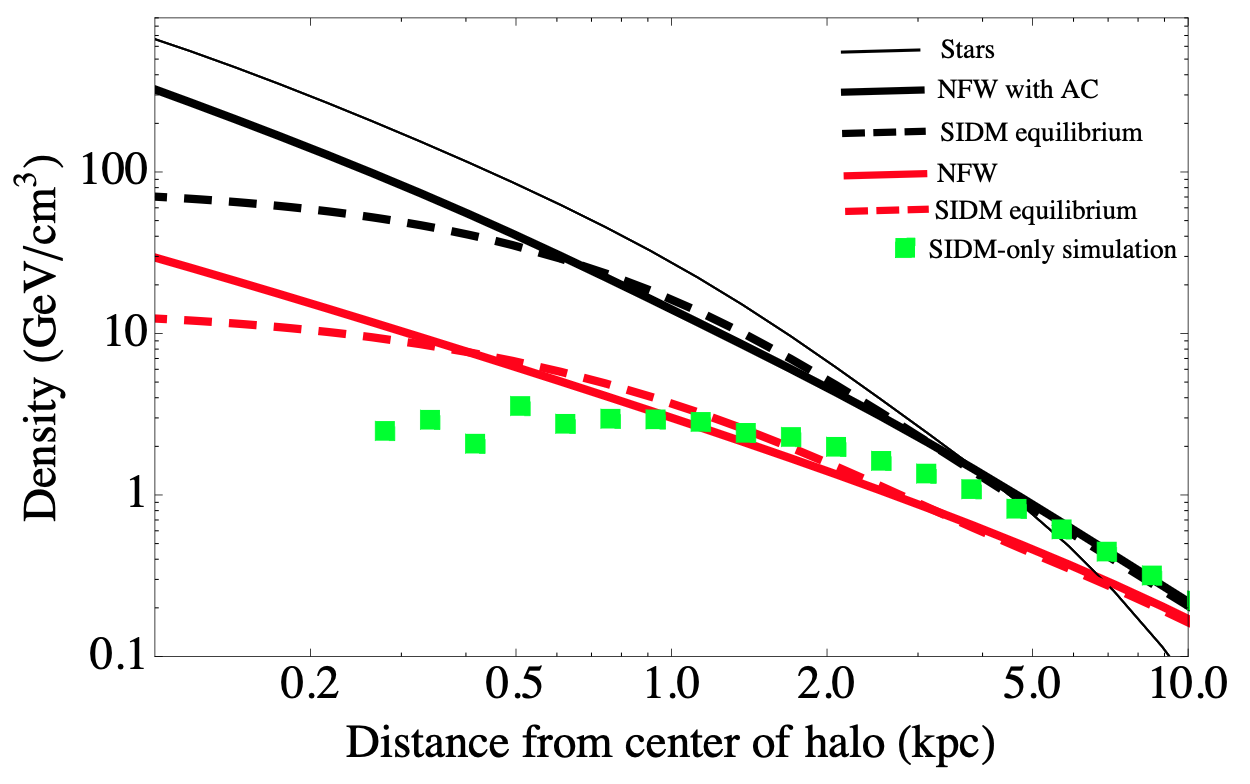
\includegraphics[width=0.65\linewidth]{figs/kaplinghat_sidm_density.png}
    \caption{%
        Mass density distributions for a Milky Way-sized halo. The green boxes
        show the result of a dark matter-only SIDM simulation. The thick solid
        lines show NFW distributions, both adiabatically contracted (black)
        and not (red). (We focus only on the non-adiabatically contracted case
        in this study.) The dashed lines show the corresponding analytic SIDM
        profiles expected from the results of the Jeans equation-based
        formalism. This figure is reproduced from Figure 1
        of~\cite{kaplinghat_tying_2014}.
    }
    \label{fig:sidm_expected_density}
\end{figure}


\hypertarget{self-interaction-in-simulation}{%
\section{Self-interaction in simulation}\label{self-interaction-in-simulation}}

In this work, we will be exploring the introduction of self-interaction in
predictions about the infall of the Sagittarius dwarf galaxy and,
specifically, the formation of its stream. This is done through the use of
N-body simulations. As such, we present a description of how these
self-interactions are modeled in simulation. We choose to use
GIZMO~\cite{hopkins_new_2015} for our simulations, and the implementation of
self-interactions therein is the one described
by~\cite{rocha_cosmological_2013}. Much of the following discussion comes in
large part from~\cite{rocha_cosmological_2013}.

In our simulation, we consider some number of ``macro-particles,'' each
of which represents an ensemble of dark matter particles, or a patch of the
dark matter phase-space density. We let each macro-particle have mass
\(m_p\), and we keep this mass consistent across all dark matter
macro-particles. Since we consider the macro-particle as representing a
patch of the phase-space density, we consider its position to be
centered at some point \(\mathbf{x}\) but spread out according to a
kernel \(W(r,h)\). Here, \(r\) is the distance from the center of the
macro-particle and \(h\) is a smoothing length.  In
GADGET-2~\cite{springel_cosmological_2005}, from which GIZMO is built and
inherits its implementation of this algorithm, the kernel is given by
\begin{equation}
W(r,h) = \frac{8}{\pi h^3} \left\{ 
    \begin{array}{ll}
        1 - 6 (r/h)^2 + 6 (r/h)^3 & 0 \leq r/h \leq 1/2, \\
        2 (1 - r/h)^3 & 1/2 < r/h \leq 1, \\
        0 & r/h > 1.
    \end{array}
\right.
\end{equation}
The smoothing length in GIZMO is fixed and on the order of $10$ pc.  The
velocity of the macro-particle is taken to instead be a delta function, such
that the macro-particles have a single defined velocity.

When the patches represented by two macro-particles overlap, we can
compute the interaction rate between them. The rate of scattering of a
macro-particle \(j\) off a target particle \(i\) is given by
\begin{equation}
\Gamma(i|j) = (\sigma/m) m_p |\mathbf{v}_i - \mathbf{v}_j| g_{ji},
\end{equation}
where \(\sigma/m\) is the familiar cross section to mass ratio and
\(g_{ij}\) is a number density factor whose purpose is account for the
overlap of the two macro-particles' smoothing kernels. It is given by
\begin{equation}
g_{ji} = \int_{0}^{h} d^3 \mathbf{x}' \, W(|\mathbf{x}'|, h) \, 
W(|\delta \mathbf{x}_{ji} + \mathbf{x}'|, h),
\end{equation}
with \(\delta \mathbf{x}_{ji}\) the displacement vector between the
macro-particle positions.

Over the course of a time step \(\delta t\), the probability of an
interaction of macro-particle \(j\) off target macro-particle \(i\) is
given by 
\begin{equation}
P(i|j) = \Gamma(i|j) \, \delta t.
\end{equation}
The total probability
of interaction between these two particles in this time step, then,
would be the average of the two directed probabilities, i.e.
\begin{equation}
P_{ij} = \tfrac{1}{2} \left( P(i|j) + P(j|i) \right).
\end{equation}
To actually
represent the interaction, then, one draws a random number and adjusts
the velocities of the particles if the number lies below the
probability. The velocities are adjusted in a manner consistent with an
elastic scattering which is isotropic in the center of mass frame.

More details are presented in~\cite{rocha_cosmological_2013}, including the
derivation of the scattering rate formula from the Boltzmann equation. We use
the implementation which is packaged with the publicly-available
GIZMO~\cite{hopkins_new_2015} simulation suite.

\hypertarget{sagittarius}{%
\chapter{Sagittarius}\label{sagittarius}}

\hypertarget{overview}{%
\section{Overview}\label{overview}}

Sagittarius (Sgr) is a dwarf spheroidal (dSph) galaxy in the Milky Way. It was
the ninth dwarf satellite discovered in the Milky Way, and the last to be
discovered before the advent of digital surveys~\cite{simon_faintest_2019}. It
was identified in 1994 by Ibata et al.~\cite{ibata_dwarf_1994} as a dwarf
satellite in the constellation of Sagittarius (hence its name). The authors
then noted that it was the closest known galaxy to the Milky Way of any known
at the time, and this has largely remained true to the present. One quirk
about Sgr that was noted at the time was that it ``is elongated towards the
plane of the Milky Way, suggesting that it is undergoing some tidal disruption
before being absorbed by the Milky Way.'' This would turn out to be a very
important feature of Sgr to explain.

In the years since, many studies have been performed to try to understand and
quantify various properties of Sgr, like its mass, orbital time, and the
reason for its elongated shape. By 2000, it was believed that the elongation
was the result of tidal shearing~\cite{jiang_orbit_2000}, meaning that
accurately describing the orbital history of Sgr is essential. Further, this
means we can expect that the stripping of stars by tidal forces may play a
significant role in its evolution. Jiang and Binney~\cite{jiang_orbit_2000}
thus explored the parameter space for the initial mass and radius of Sgr,
finding that a wide range of parameters are possible, from an initial mass of
\(\sim 10^{11}\) M\(_\odot\) and Galactocentric distance of \(\gtrsim 200\)
kpc to mass \(\sim 10^9\) M\(_\odot\) and distance \(\sim 60\) kpc.

Shortly thereafter, Majewski et al.~used the Two Micron All Sky Survey (2MASS)
to map Sgr, forming the first canonical model of Sgr~\cite{majewski_two_2003}.
Their characterization of Sgr included a description of a \emph{stream} of
stars that had been tidally stripped from Sagittarius, forming leading and
trailing ``tidal tails''. These tails, they note, ``lie along a well-defined
orbital plane about the Galactic center.'' Moreover, they state that the lack
of precession in the tidal debris is indicative of a nearly spherical
gravitational potential for the Milky Way, recognizing the usefulness of the
Sagittarius stream as a potential measure of the gravitational potential. 

We have included a reproduction of Figure 11 from~\cite{majewski_two_2003}, a
plot of a sample of Sgr debris stars in the orbital plane. It can be seen in
Figure~\ref{fig:majewski}. The core of Sgr lies at approximately $(+20, -10)$ in
the plot coordinates, with the northern arm leading above it and the southern
arc leading to the left. The Galactic center is located at $(0, 0)$.

\begin{figure}
    \centering 
    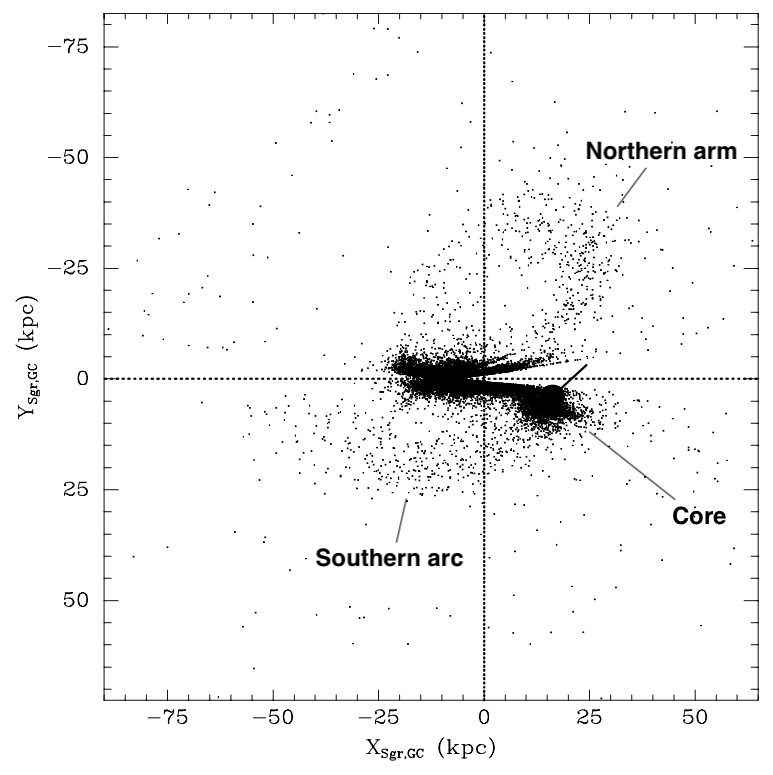
\includegraphics[width=0.45\linewidth]{figs/majewski2003-11.png}
    \caption{%
        Sgr debris in the orbital plane with the Galactic center at the
        origin. Reproduced from Figure 11 of~\cite{majewski_two_2003}.
    }
    \label{fig:majewski}
\end{figure}

todo Belokurov et al.~2006

The picture of Sagittarius as tidally disrupted with debris forming a long
streaming arc about the Milky Way would turn out to be well-supported by
further observations and studies. In the ensuing years, more studies were
performed to improve the model and more accurately quantify the properties of
the galaxy. We note in particular the work of Kunder and
Chaboyer~\cite{kunder_distance_2009} who estimated the distance to Sgr to be
approximate 24.8 kpc.

todo add a discussion of stream coordinates?

\hypertarget{modern-models}{%
\section{Modern models}\label{modern-models}}

The next major discovery in the history of Sagittarius was the 2010 Law and
Majewski model~\cite{law_sagittarius_2010}. This model became the first two
successfully satisfy the majority of existing constraints on the angular
position, distance, and radial velocity of the tidal debris streams. It did so
using a triaxial Milky Way halo; in other words, it dropped the typical
assumption that the Milky Way halo is axisymmetric in the Galactic plane. One
prediction of note from this model is that the current bound mass of Sgr is
approximately \(2.5 \times 10^8\) M\(_\odot\). To obtain this, they use an
initial mass of \(6.4 \times 10^8\) M\(_\odot\) with an infall orbit for
around 8 Gyr in a fixed Galactic gravitational potential. It is worth noting
that this initial mass lies in the régime where dynamical friction is small
and the effects of tidal stripping on the Sgr progenitor are relatively
small~\cite{dierickx_predicted_2017}.

The resulting distribution of stars is shown in Figure~\ref{fig:law}. We
reproduce their plots of the debris stream in terms of heliocentric
coordinates and Galactocentric distances in the orbital plane. The coloring
corresponds to the time at which the debris was stripped from Sgr. (Green is
between the first and third apocenters, cyan between the third and fifth,
magenta between the fifth and seventh, and orange later than the seventh.)
Notice as well that they predict \textit{two} wraps for both the leading
(``L'') and trailing (``T'') stream arms.

\begin{figure}
    \centering 
    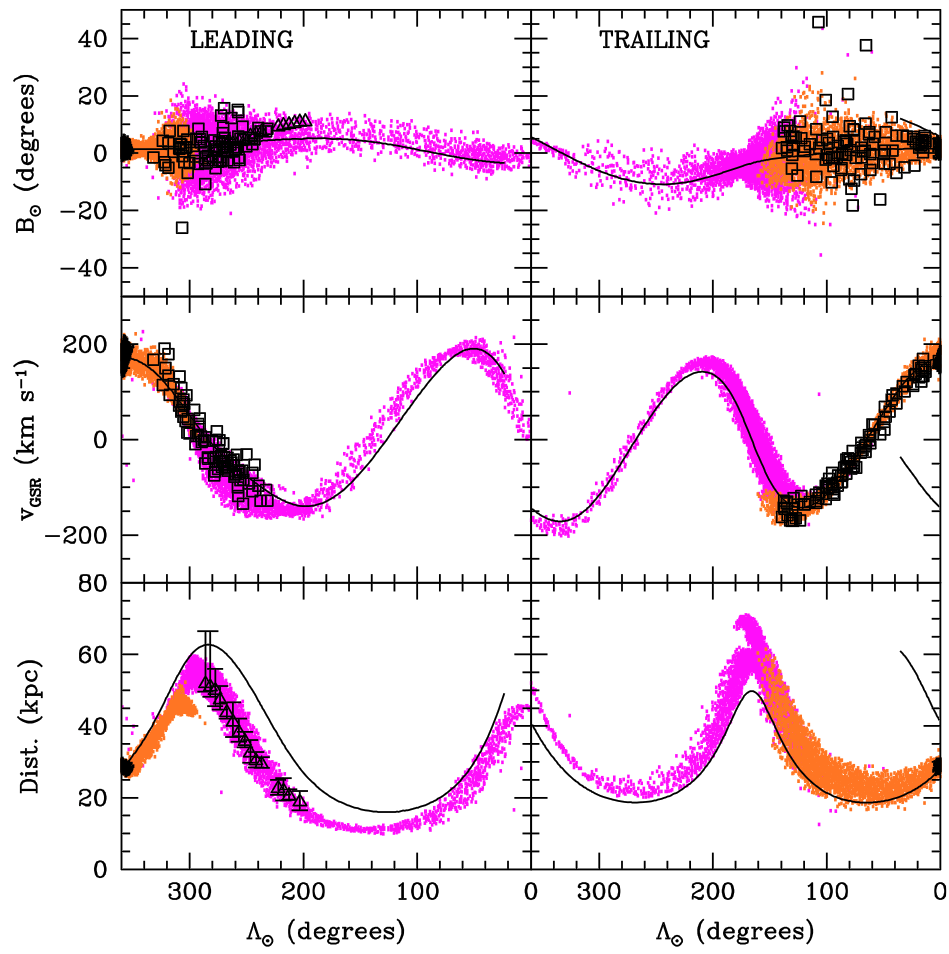
\includegraphics[width=0.45\linewidth]{figs/law2010-6.png}
    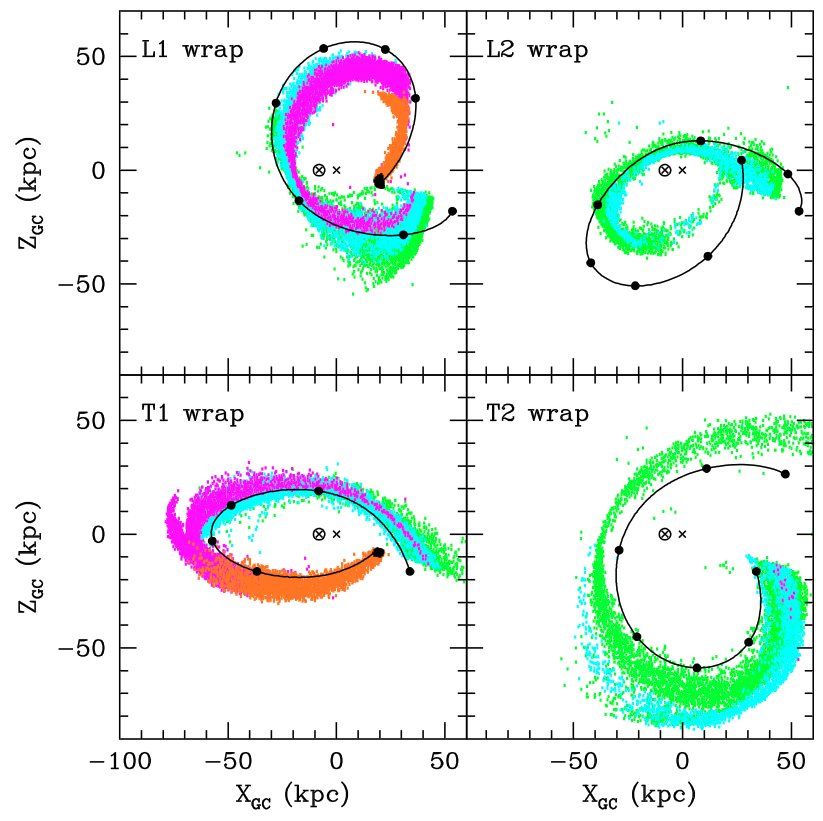
\includegraphics[width=0.45\linewidth]{figs/law2010-8.png}
    \caption{%
        Sgr stellar debris streams according to the Law and Majewski 2010
        model. On the left, debris stripped in the last $\sim 3$ Gyr is shown
        in terms of stream coordinates. On the right, the first two wraps of
        the leading (``L'') and trailing (``T'') stream arms are shown in the
        orbital plane. These plots are reproduced from Figures 6 and 8
        of~\cite{law_sagittarius_2010}.
    }
    \label{fig:law}
\end{figure}

Shortly thereafter came the model of Purcell et
al.~\cite{purcell_sagittarius_2011}. In their model, they explicitly account
for the impact of the infall of Sagittarius on the evolution of the Milky Way
disk, pointing out that all then-existing models of Sgr assume that its
effects on the Galactic disk morphology are negligible. They found that Sgr
created ``significant perturbations to the outer disk'' with noticeable
effects on the evolution of the inner spirality. In their model, Sgr is
represented as beginning with halo mass \(10^{10.5}\) M\(_\odot\) at a
Galactocentric radius of 80 kpc in the Galactic plane. In order to account for
tidal stripping that would have occurred between the infall of Sgr past the MW
virial radius and the starting position they choose, they truncate the initial
halo at the instantaneous Jacobi radius, \(r_t = 23.2\) kpc. We note that such
methods may produce qualitatively accurate representations of Sgr but are
unlikely to accurately reflect the true orbital history of Sgr.

The resulting stream debris is shown in Figure~\ref{fig:purcell}. We show again
both the stream in terms of heliocentric coordinates and in the orbital plane in
terms of Galactocentric distances. We focus in particular on the ``light Sgr''
subplot of the Galactocentric figure. The figures show qualitatively similar
patterns to the model of Law and Majewski~\cite{law_sagittarius_2010}, including
the ``L1'' and ``T1'' wraps.

\begin{figure}
    \centering 
    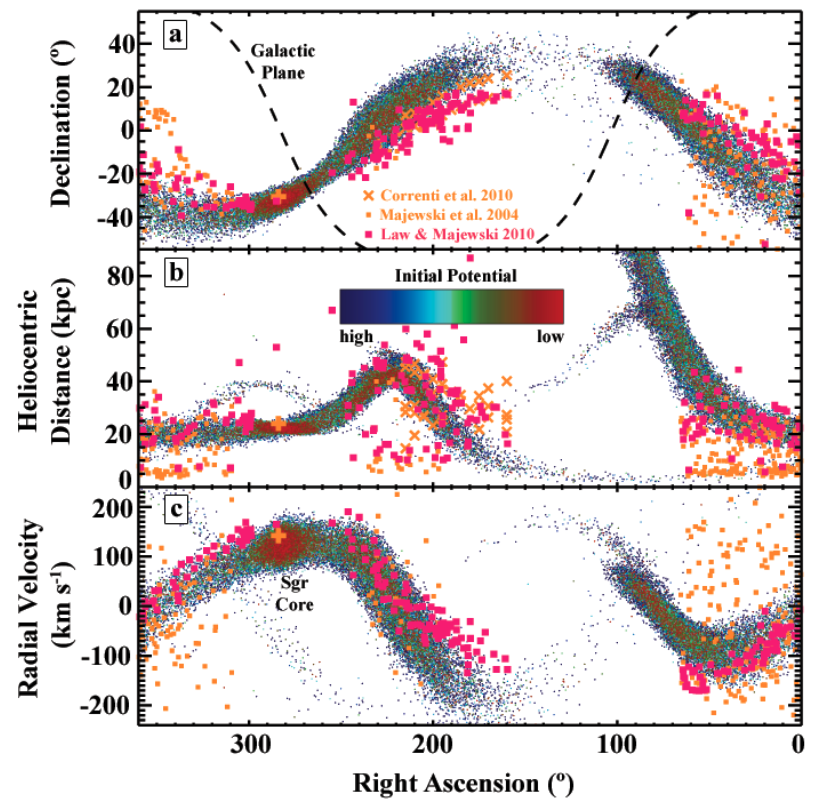
\includegraphics[width=0.41\linewidth]{figs/purcell2011-3.png}
    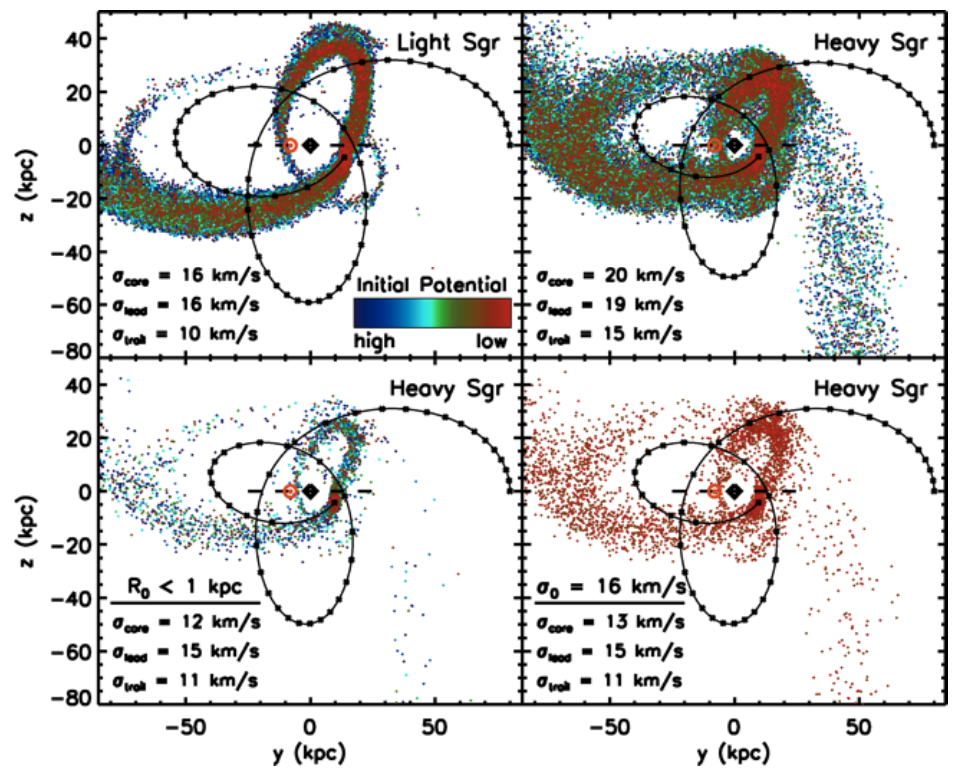
\includegraphics[width=0.5\linewidth]{figs/purcell2011-s4.png}
    \caption{%
        Sgr stellar debris streams according to the Purcell et al.~2011 model.
        On the left, debris is shown in terms of heliocentric coordinates. On
        the right, the debris is shown in terms of Galactocentric distances in
        the orbital plane. We note in particular that the debris appears to
        contain approximately the same shape as the ``L1'' and ``T1'' wraps of
        the Law model. Figures reproduced from Figures 3 and S4
        of~\cite{purcell_sagittarius_2011}.
    }
    \label{fig:purcell}
\end{figure}

todo belokurov 2014 ?

As such, the status until quite recently was that no existing Sagittarius
model did could accurately account for a live Milky Way potential, the effects
of dynamical friction, and the early infall of Sgr at Galactocentric radii of
more than 60-80 kpc. In 2017, however, a new model which sought to solve all
these problems was found by Dierickx and Loeb~\cite{dierickx_predicted_2017}.
They simulate the infall of Sagittarius starting from its first crossing of
the Milky Way virial radius approximately 8 Gyr ago using a live Milky Way
gravitational potential and accounting for the full effects of dynamic
friction. To find the best-fit model, they began by performing a parameter
search with a fast and simple semi-analytic model. They then used these
best-fit parameters in a full, high-resolution N-body simulation.

The resulting simulation is able to reproduce both the leading and trailing
stream arms to good agreement with both observed data and past models.
Moreover, they note that the resulting model is the first to accurately
reproduce existing data for debris observed 100 kpc away. The model also
predicts the existence of an extension to the stream, including ``the
existence of several arms of the Sgr stream extending to hundreds of
kiloparsecs.'' They note that this predicted structure matches the positions
of the two most distant stars known in the Milky Way halo and serves as a
testable prediction for data from future sky surveys.

This model is the one that we have (approximately) chosen to adopt for our
simulations. The specific differences between our model and theirs will be
elucidated in (todo add reference to simulation section). Dierickx and Loeb
represent the Milky Way halo using a Hernquist distribution with total mass
\(1.25 \times 10^{12}\) M\(_\odot\) and scale radius 38.35 kpc. The Milky Way
disk follows an exponential profile with mass \(8.125 \times 10^{10}\)
M\(_\odot\), scale length 3.5 kpc, and scale height 0.525 kpc. They also use a
Hernquist bulge with mass \(1.25 \times 10^{10}\) M\(_\odot\) and scale length
0.7 kpc. In their model, Sagittarius has a Hernquist halo with total mass
\(1.3 \times 10^{10}\) M\(_\odot\) and scale radius 9.81 kpc. It has an
exponential disk with mass \(6 \times 10^{8}\) M\(_\odot\), scale length 0.85
kpc, and scale height 0.1275 kpc, and a Hernquist bulge with mass \(5.2 \times
10^{8}\) M\(_\odot\) and scale length 0.17 kpc.

As before, we include plots of the resulting stellar debris, both in terms of
heliocentric coordinates and Galactocentric distances in the orbital plane.
These plots are given in Figure~\ref{fig:dierickx}. In this case, the familiar
stream structure is once again reproduced, but with the inclusion of a
significant extension to the stream arms far beyond the two wraps considered
by Law and Majewski. The resulting distribution also appears to approximately
reproduce the distributions of observed stars (observational data shown in
black).

\begin{figure}
    \centering 

    \begin{subfigure}{0.43\textwidth}
        \centering
        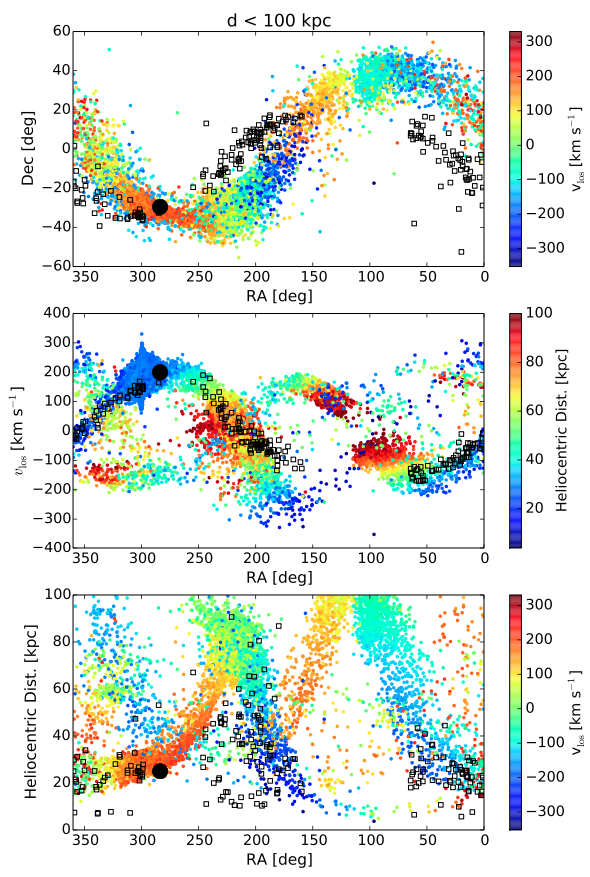
\includegraphics[width=\textwidth]{figs/dierickx2017-10.png}
    \end{subfigure}
    \begin{subfigure}{0.52\textwidth}
        \centering
        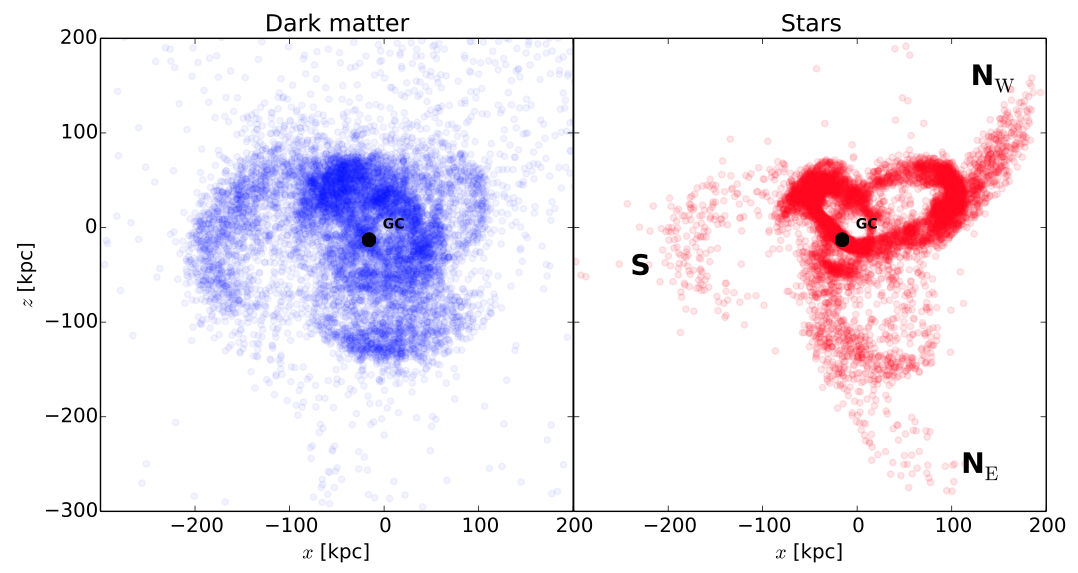
\includegraphics[width=\textwidth]{figs/dierickx2017-8.png}
        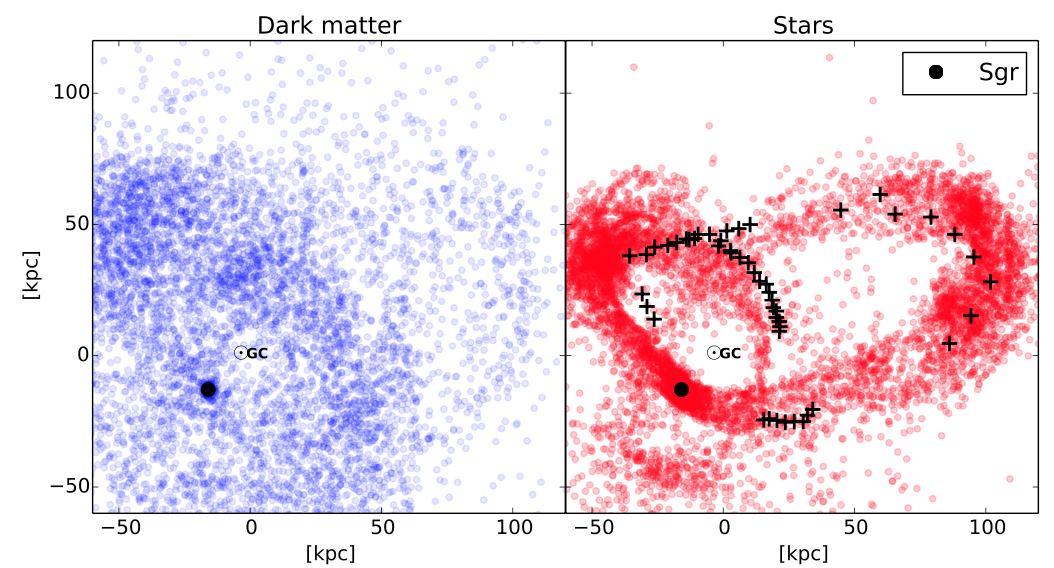
\includegraphics[width=\textwidth]{figs/dierickx2017-9.png}
    \end{subfigure}

    \caption{%
        Sgr stellar debris according to the Dierickx and Loeb 2017 model. As
        before, we show the stream in heliocentric coordinates on the left. On
        the right is the stream (and associated dark matter particles) in terms
        of Galactocentric distances in the orbital plane. The right top
        subfigure shows the full distributions, while the right bottom subfigure
        zooms into the more observationally relevant region. Comparisons to
        observed Sgr stars are also shown in black. Plots reproduced from
        Figure 8, 9, and 10 of~\cite{dierickx_predicted_2017}.
    }
    \label{fig:dierickx}
\end{figure}

\hypertarget{simulation-setup}{%
\chapter{Simulation setup}\label{simulation-setup}}

As stated previously, the core work of this thesis is performing N-body
simulations of the infall of Sgr in the style of Dierickx et
al.~\cite{dierickx_predicted_2017}, varying the initial conditions and dark
matter model to determine the resulting impacts on the evolution of the Sgr
tidal debris stream. As such, we provide an overview of the setup of the
simulations we performed in this section.

\hypertarget{pipeline-and-parameters}{%
\section{Pipeline and parameters}\label{pipeline-and-parameters}}

To begin our experimental pipeline, we first generate the initial
distributions of stellar and dark matter particles using a package called
GalactICS~\cite{deg_galactics_2019}. Each galaxy is modeled using a stellar
disk and dark matter halo. The halo follows a Navarro-Frenk-White (NFW)
profile
\begin{equation}
    \rho_{\text{halo}} (r) = 
    \frac{M_{200}}{4\pi a^3 f(c)} 
    \frac{1}{(r/a)(1+r/a)^2},
\end{equation}
where $f(c) = \log (1+c) - c/(1+c)$, $M_{200}$ is the virial mass, $a$ is the
scale length, $c$ is the concentration, and $c = r_{200} / a$. Here, we use a
lowercase $r$ to denote the radius in a spherical sense.

The stellar disk follows an exponential-sech$^2$ profile, given by
\begin{equation}
    \rho_{\text{disk}} (R, z) = 
    \frac{M_{\text{disk}}}{4 \pi R_0^2 z_0}
    \exp(-R/R_0) \text{ sech}^2(z/z_0),
\end{equation}
where $R_0$ is the disk scale length, $z_0$ is the disk scale height, and the
capital $R$ denotes the cylindrical radius in the plane of the disk.

Both of these distributions are subject to truncation beyond a certain
radius, \(r_t\), with truncation width \(dr_t\). The truncation function
comes from~\cite{widrow_dynamical_2008} and is given by
\begin{equation}
C(r; r_t, dr_t) = \frac{1}{2} \text{erfc} 
\left( \frac{r - r_t}{\sqrt{2} dr_t} \right).
\end{equation}
For the halos, the truncation radius is simply the virial radius and the
truncation width is 20 kpc. For the disks, the truncation radius is 25 kpc,
the width is 5 kpc, and the truncation is only applied to $R$ in the disk
plane. The distributions, including the truncation parameter, can be seen in
Figure~\ref{fig:init_profiles}.

\begin{figure}
    \centering
    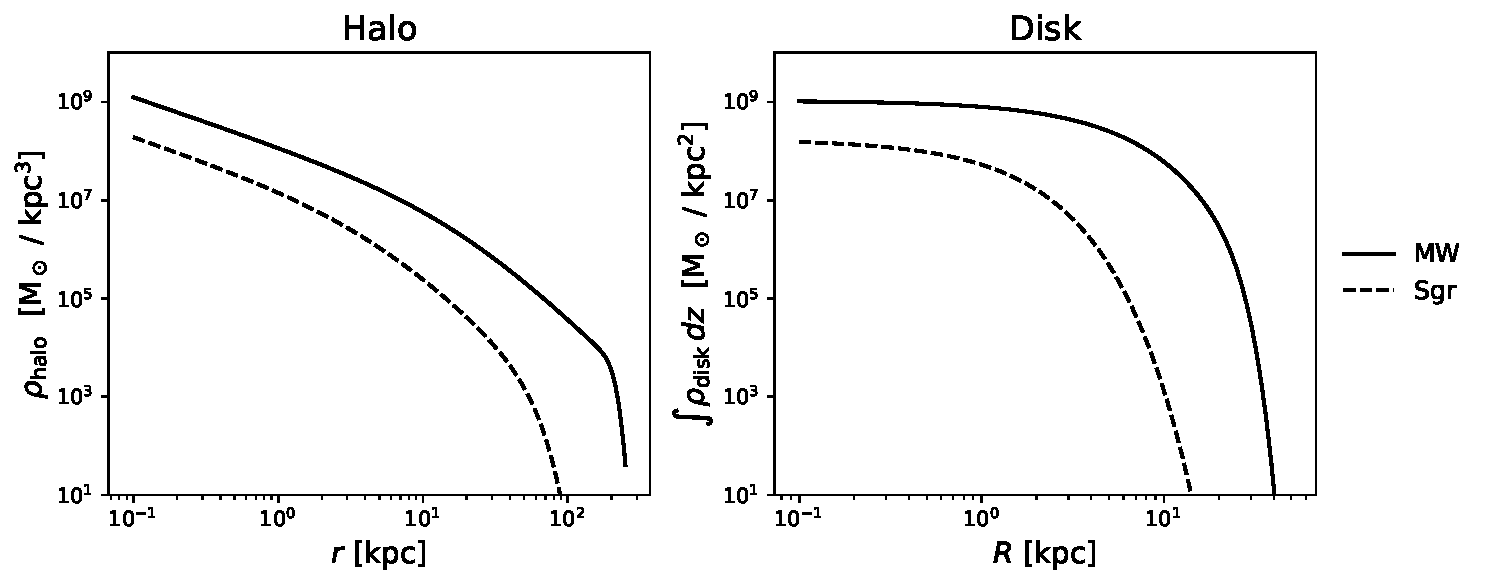
\includegraphics[width=0.9\linewidth]{figs/init_profiles.pdf}
    \caption{%
        Initial profiles for the halo and disk of both galaxies. The halos
        follow a truncated NFW profile and the disks follow a truncated
        exponential-sech$^2$ profile. Note that the disk density is in
        cylindrical coordinates and is integrated over the $z$ direction.
    }
    \label{fig:init_profiles}
\end{figure}

Bundled with GalactICS is a subpackage called GadgetConverters, which
provides a pipeline for converting the native output of GalactICS into a
binary compatible with GADGET and derivative N-body simulation software. In
this work, we use GIZMO~\cite{hopkins_new_2015}, which is itself derived from
GADGET-2~\cite{springel_cosmological_2005}.

\begin{table}
\centering
\begin{tabular}{lcll}
    \toprule
    Parameters & & MW & Sgr \\
    \midrule 
    Halo \\
    $\quad$ Virial mass & $M_{200}$ & $10^{12}$ M$_\odot$ & $10^{10}$ M$_\odot$ \\
    $\quad$ Virial radius & $r_{200}$ & 206 kpc & 44 kpc \\
    $\quad$ Concentration & $c$ & 10 & 8 \\
    $\quad$ Particles & $N_{\text{halo}}$ & $1.16 \times 10^{6}$ & $1.17 \times
    10^{4}$ \\
    Disk \\
    $\quad$ Mass & $M_{\text{disk}}$ & $6.5 \times 10^{10}$ M$_\odot$ & $6 \times 10^{8}$ M$_\odot$ \\
    $\quad$ Scale length & $R_0$ & 3.5 kpc & 0.85 kpc \\
    $\quad$ Scale height & $z_0$ & 0.53 kpc & 0.13 kpc \\
    $\quad$ Particles & $N_{\text{disk}}$ & $2.03 \times 10^{6}$ & $1.17 \times
    10^{4}$ \\
    \bottomrule
\end{tabular}
\caption{%
    Parameters for the initial Milky Way and Sgr galaxies in our full
    simulation. These values are in large part taken from the work
    of~\cite{dierickx_predicted_2017}.
}
\label{tab:sim_params}
\end{table}

The parameters that were used for our simulations were largely taken from the
work of Dierickx et al.~\cite{dierickx_predicted_2017}. They are summarized in
Table~\ref{tab:sim_params}. There are a few key differences between their model
and our simulations, however. First, they used Hernquist profiles for their
halos, while we use NFW distributions. The NFW parameters we use, however, come
from their work, where they are given as the parameters which yield an
approximately equivalent distribution. A comparison between their Hernquist
and our NFW profiles is shown in Figure~\ref{fig:nfw_vs_hernquist}; the
differences are quite small.

\begin{figure}
    \centering
    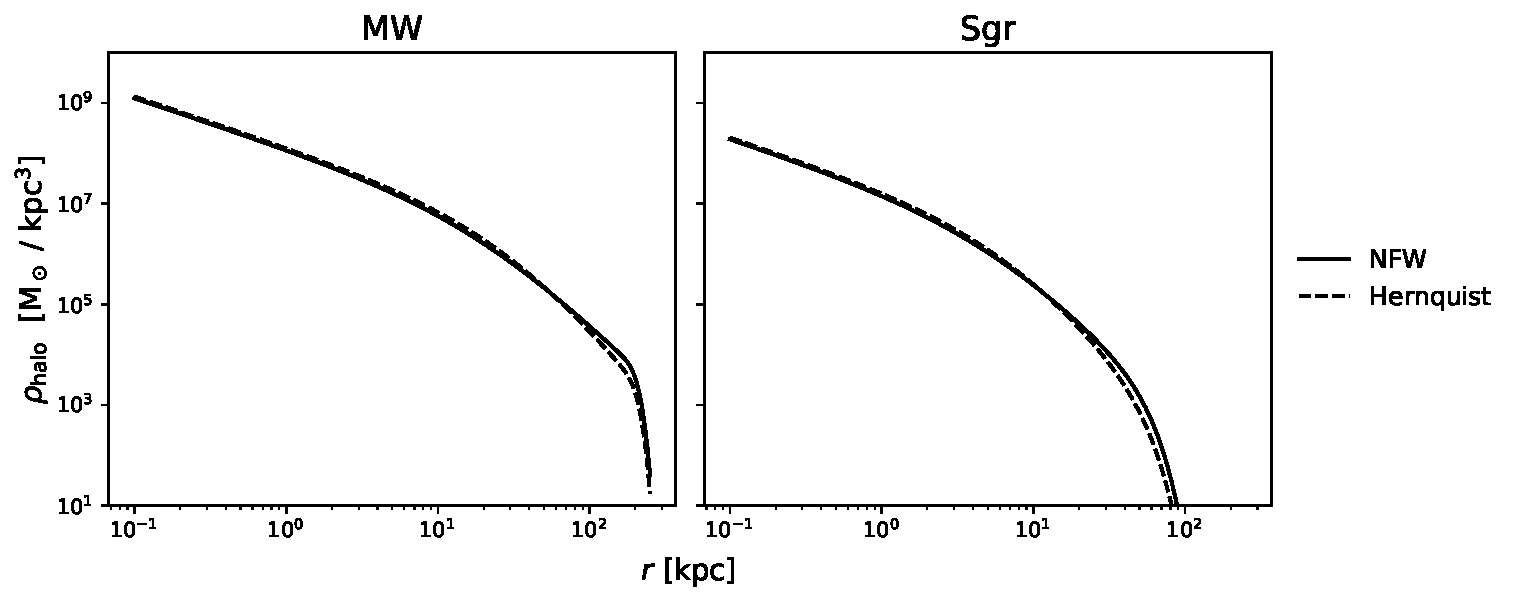
\includegraphics[width=0.9\linewidth]{figs/nfw_vs_hernquist.pdf}
    \caption{%
        Comparison between the density profiles of the relevant truncated NFW
        and truncated Hernquist profiles for the Milky Way and Sgr galaxies in
        the Dierickx model. The NFW parameters can be found in
        Table~\ref{tab:sim_params}. The Hernquist parameters are as follows:
        total MW halo mass $1.25 \times 10^{12}$ M$_\odot$, MW scale radius
        $38.35$ kpc, total Sgr halo mass $1.3 \times 10^{10}$ M$_\odot$, Sgr
        scale radius $9.81$ kpc.
    }
    \label{fig:nfw_vs_hernquist}
\end{figure}

The second source of discrepancy between their work and ours is that we have
less resolution in our stellar profile than in their work. This is in part
because they used a Hernquist bulge in both their Milky Way and Sgr, where this
has been omitted from our work. It is also because they used more stellar
particles for the Sgr disk than we did ($1.94 \times 10^4$ versus $1.17 \times
10^4$), owing to a technical error in our initial conditions creation
pipeline.

The experiments performed herein were performed using GIZMO version
2020, built from commit master:0e19830, on Princeton Research Computing's
Della cluster.  This cluster is an Intel cluster with $\geq 20$ cores per node
and $\geq 128$ GB memory per
node~\cite{princeton_research_computing_della_nodate}.  Our simulations often
used around 10 GB of RAM and typically split the computation over 25 cores.

\hypertarget{equilibration}{%
\section{Equilibration}\label{equilibration}}

After generating the initial particle distributions for each galaxy, we
evolved each one forward in time for several Gyrs to allow it to equilibrate.
One reason we do this is because generating initial conditions which are in
equilibrium is a difficult problem, and the initial conditions generator we use
only gives an approximately equilibrated distribution. Evolving it forward in an
isolated system allows the galaxy to come to equilibrium naturally. We have seen
this to be necessary particularly for the Sgr disk distributions.  Another
reason we choose to do this is to create a cored dark matter profile when
using SIDM microphysics.

For each galaxy, we begin with the parameters discussed in the previous
section and perform two equilibration runs: one using CDM microphysics and one
using SIDM microphysics with a velocity independent cross section of \(\sigma
/ m = 10\) cm\(^2\)/g.  In this study, we choose to use a somewhat high cross
section in order to exaggerate any differences that may appear because of the
presence of self-interaction.  We note that future studies should consider a
range of cross sections and velocity dependence.

For the Milky Way equilibrations---both CDM and SIDM---we only evolve the
galaxy forward for 1 Gyr, writing time stamps approximately every 0.1 Gyr.
This is because we expect the initial distribution to be relatively close to
equilibrium, especially when considering such a large galaxy. The resulting
evolution of the mass density profiles are shown in Figure~\ref{fig:mw_evo}.

\begin{figure}
    \centering
    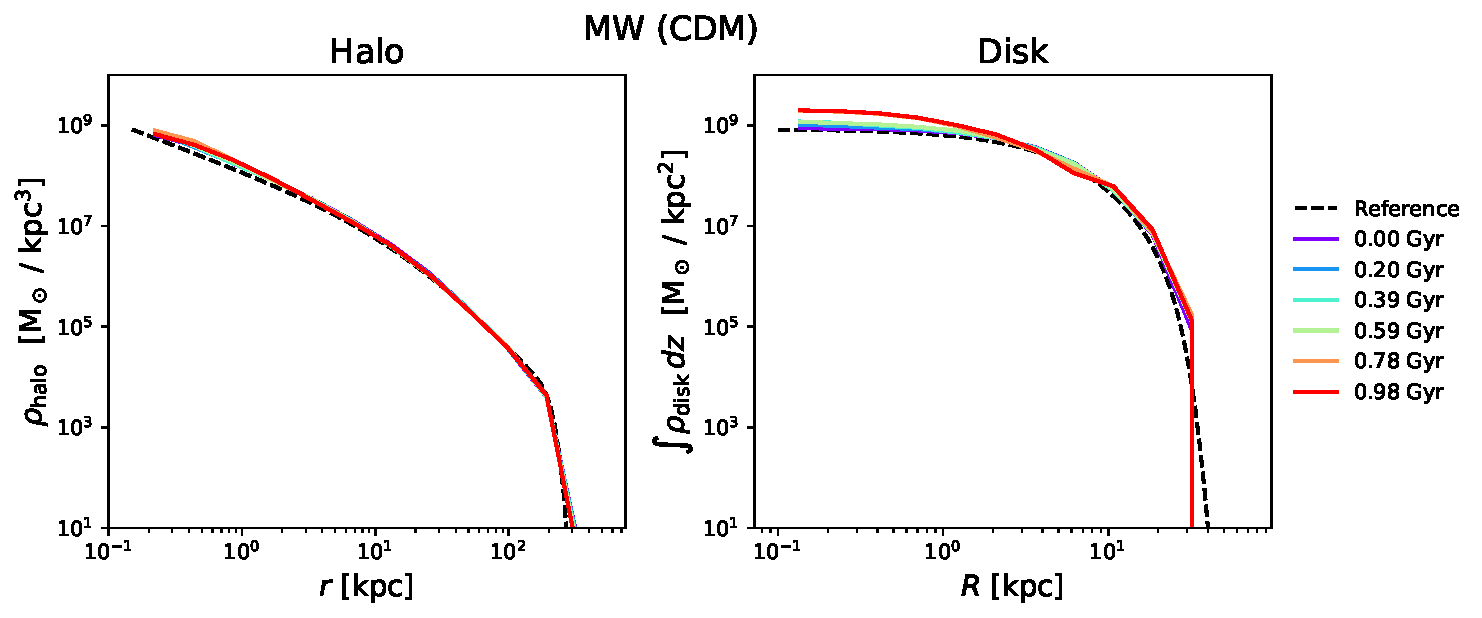
\includegraphics[width=0.9\linewidth]{figs/mw_evolution_cdm.pdf}
    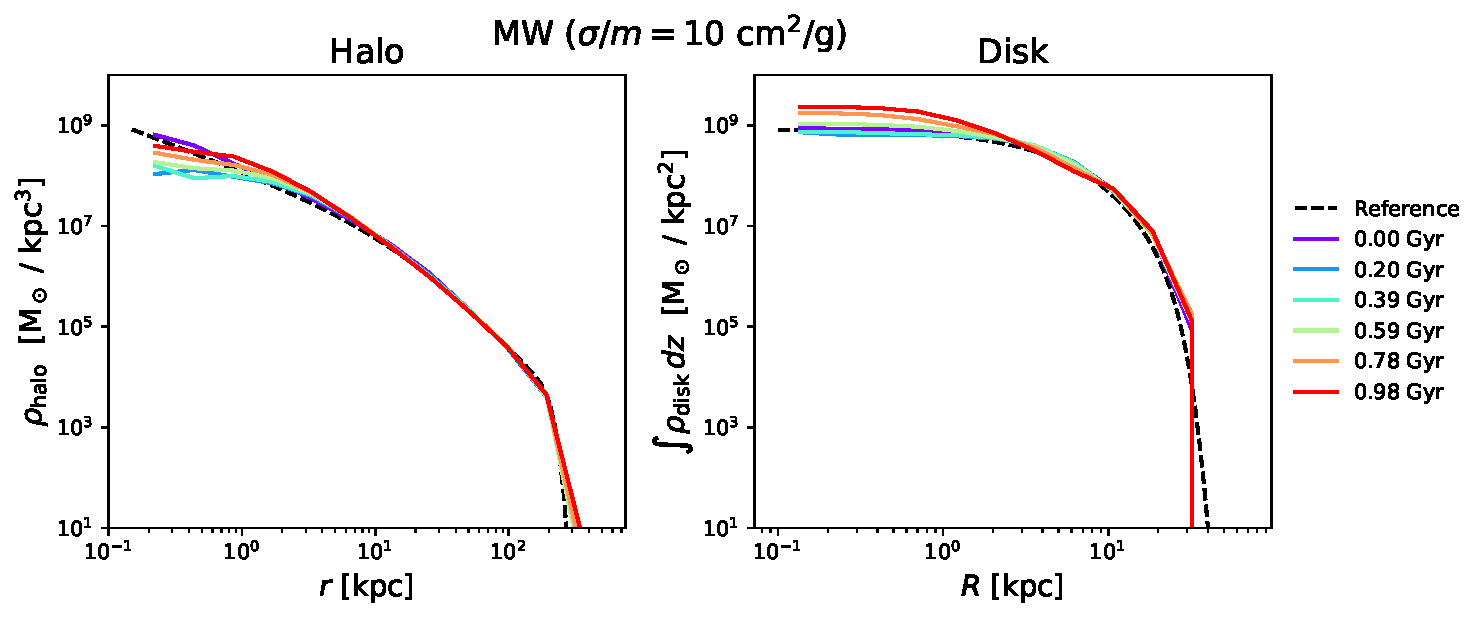
\includegraphics[width=0.9\linewidth]{figs/mw_evolution_sidm.pdf}
    \caption{%
        Evolution of the MW halo (left) and disk (right) during CDM (top) and
        SIDM (bottom) equilibration runs. The dashed line on the halo plots is
        the reference NFW distribution; on the disk plots it is the reference
        exponential-sech$^2$ distribution.
    }
    \label{fig:mw_evo}
\end{figure}

In these plots, we can see that the CDM halo starts in a state which is already
close to equilibrium. The halo changes very little, and the disk slowly pulls
a small amount of density in toward the center. The SIDM halo, however, almost
immedately develops a rather substantial core, which slowly dissolves somewhat,
leaving a small core with size $\sim 1$ kpc. This is almost certainly because
of the disk. As the disk equilibrates, its central density increases,
increasing the gravitational potential in the center of the galaxy and
counteracting the coring effect of self-interactions.

We can also compare these results to those we might have expected following the
analytic formalism for determining the core size in
Section~\ref{analytic-description-with-baryons}. To begin, we need to find the
scale radius $r_0$ and the center value of the gravitational potential
$\Phi_B(0)$ in the ``spherical disk'' approximation. We can do so by using the
following two relations:
\begin{gather}
    \Phi_B(0) = - \frac{G M_B}{r_0} \\
    V_B(r_0) = \frac{\sqrt{-\Phi_B(0)}}{2},
\end{gather}
where $M_B$ is the mass of the baryons in the disk and $V_B$ is the circular
velocity of baryons at the given radius. Together, these imply that $V_B(r_0) =
\sqrt{G M_B / 4 r_0}$.  After truncation, our disk has a total mass of $M_B =
8.1 \times 10^{10}$ M$_\odot$.  Thus, we can plot the rotation curve of our
disk and look for its intersection with $\sqrt{G M_B / 4 r_0}$.  This should
give us the values of $r_0$ and $V_B(r_0)$.  The rotation curves for both the
CDM and SIDM curves are plotted in Figure~\ref{fig:mw_rot_curves}. They show
$r_0 \approx 3.5$ kpc with a corresponding circular velocity $V_B(r_0) \approx
160$ km/s. 

\begin{figure}
    \centering 
    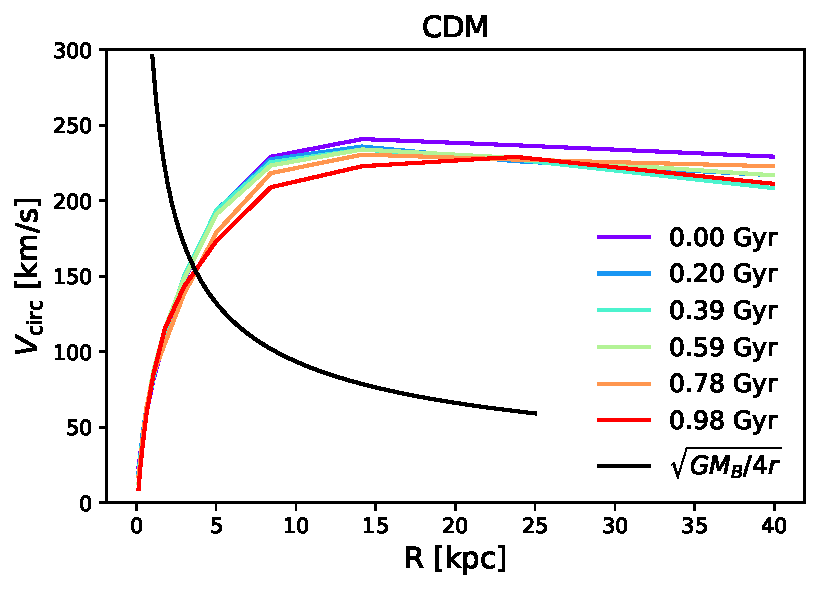
\includegraphics[width=0.45\linewidth]{figs/mw_cdm_rot_curve.pdf}
    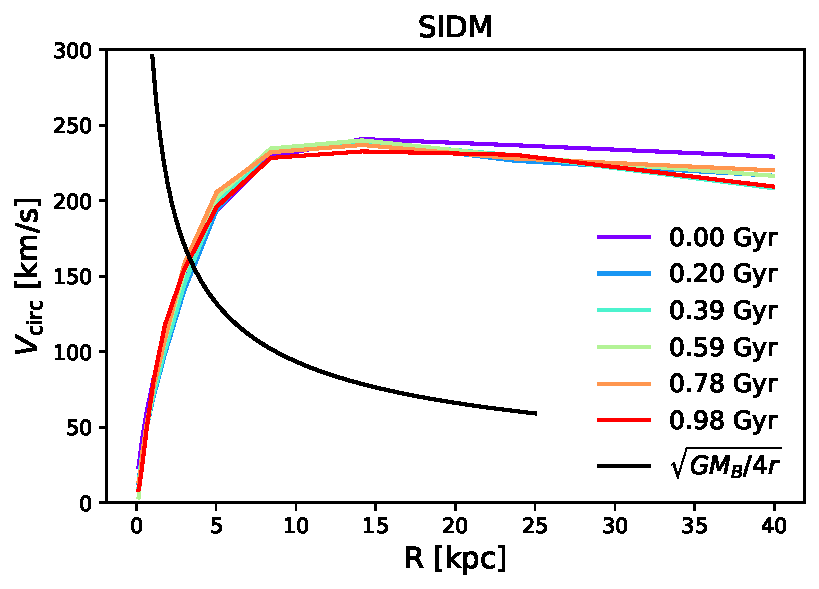
\includegraphics[width=0.45\linewidth]{figs/mw_sidm_rot_curve.pdf}
    \caption{%
        Evolution of rotation curves over time for the Milky Way disk in both
        the CDM and SIDM microphysics runs. Also plotted in black is
        $\sqrt{GM_B/4r}$, the circular velocity at the scale radius which would
        be expected if the disk mass followed a Hernquist profile.
    }
    \label{fig:mw_rot_curves}
\end{figure}

Looking back at Figure~\ref{fig:mw_evo}, we can estimate the central density
of the halo to be $\rho_0 \approx 10^9$ M$_\odot$/kpc$^3$. We can also compute
the central velocity dispersion by finding the root mean square of the radial
velocities for the stars in the inner 5 kpc. For the late CDM snapshots, this
measure gives $\sigma_0 = 123$ km/s.  With all these quantities, we can
compute $a_0 = 43.8$ and $a_1 = 6.6$. Plugging these in to
Equation~\ref{eq:core_size}, we obtain an estimate for the core size of $0.37$
kpc. This core size appears to be roughly consistent with the observed core
size attained in the fully evolved SIDM distribution, though perhaps a little
smaller.

For the Sgr equilibrations, however, we evolved the galaxy much farther
forward in time: approximately 10 Gyr for the CDM case and 20 Gyr for SIDM.
These evolution times do not correspond to a physical orbit (especially given
that the SIDM case would exceed the lifetime of the Universe).  Rather, the
initial Sgr disk distribution was found to be a bit unstable.  We also wanted
to be absolutely certain that the SIDM case would develop a cored profile.
The evolution of the resulting Sgr mass profiles is shown in
Figure~\ref{fig:sgr_evo}.

\begin{figure}
    \centering
    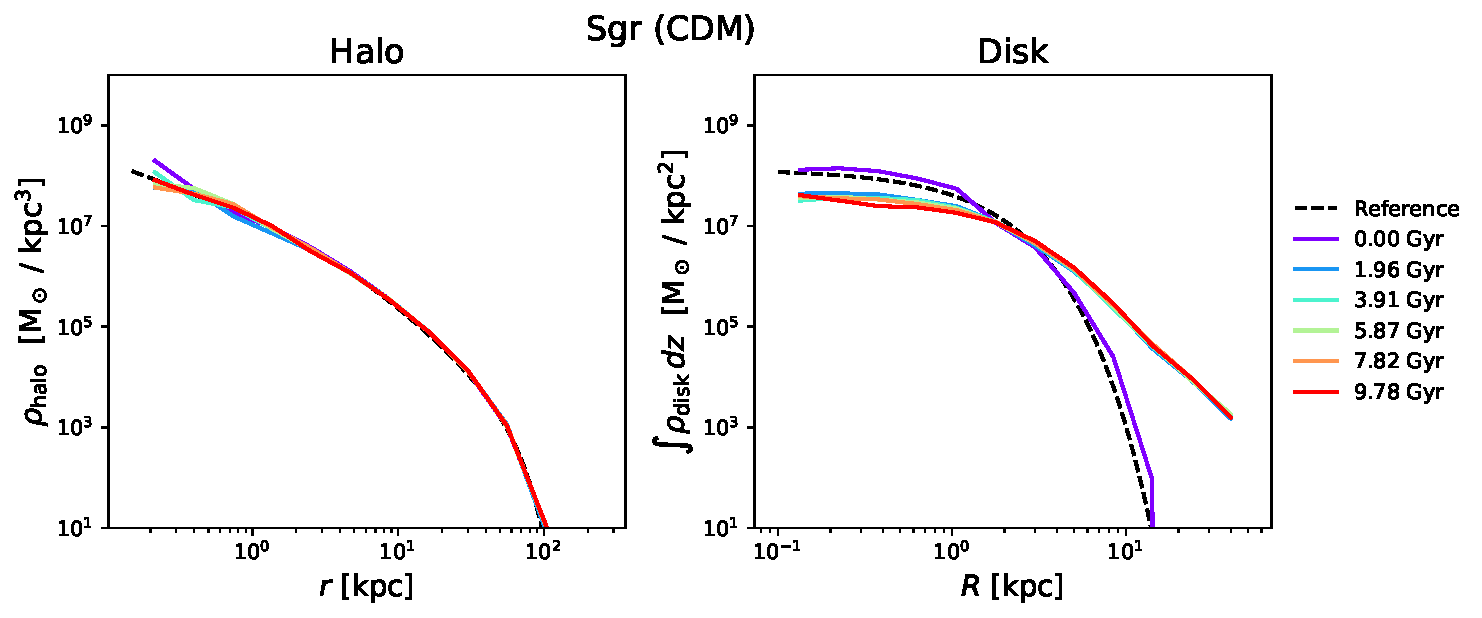
\includegraphics[width=0.9\linewidth]{figs/sgr_evolution_cdm.pdf}
    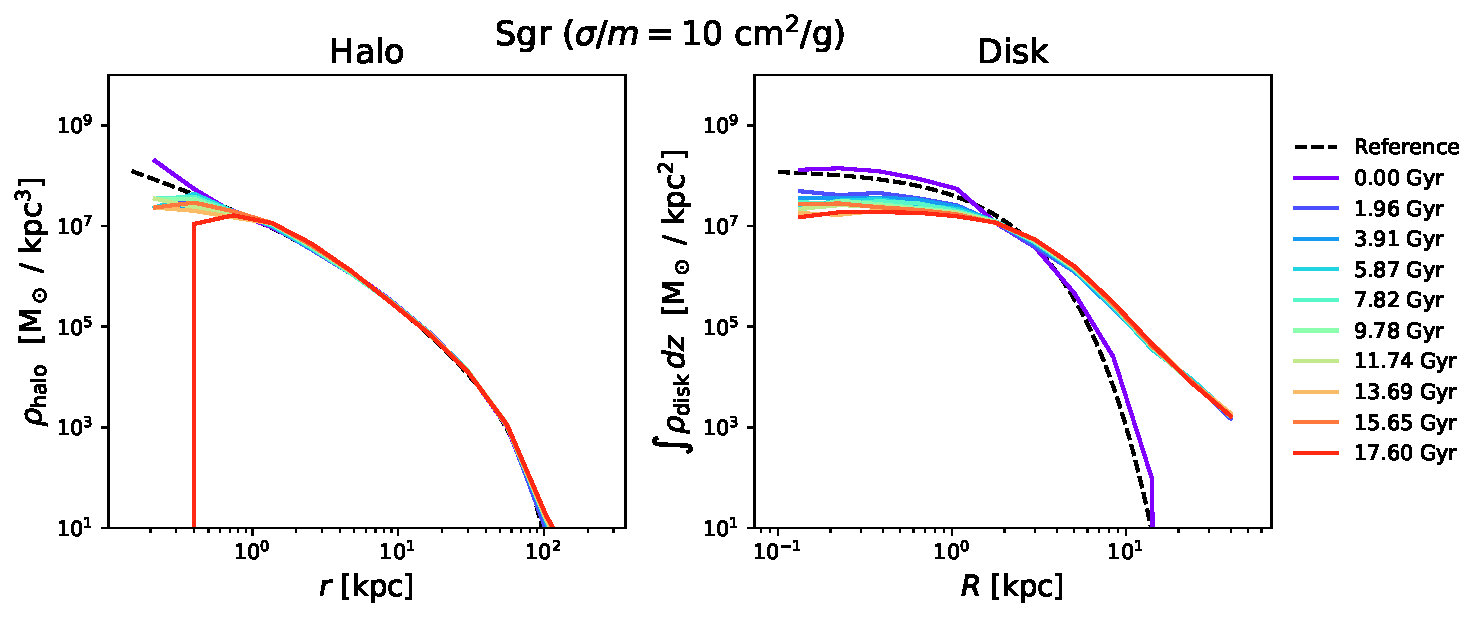
\includegraphics[width=0.9\linewidth]{figs/sgr_evolution_sidm.pdf}
    \caption{%
        Evolution of the Sgr halo (left) and disk (right) during CDM (top) and
        SIDM (bottom) equilibration runs.  The dashed line on the halo plots
        is the reference NFW distribution; on the disk plots it is the
        reference exponential-sech$^2$ distribution.  We note in particular
        that the SIDM run results in generally depressed densities for both
        the halo and disk at low radii.
    }
    \label{fig:sgr_evo}
\end{figure}

In these plots, we see that the initial exponential-sech$^2$ distribution for
the disk was not very close to equilibrium. Almost immediately, the disk
redistributes itself more outwardly, with more of its mass at larger radii and a
falling inner density. In the case of CDM physics, this happens within the first
two Gyr, and the distribution holds relatively constant from there on. In the
SIDM case, however, the distribution appears to continue to adjust, with the
central density falling to around half that of the CDM disk.

In the case of the halo, we notice that the distribution holds relatively
constant in the CDM case and agrees well with the reference NFW distribution. In
the SIDM case, however, we see the slow development of a small core at low
radii. This core appears to have a size of $\approx 1$ kpc. 

We can again apply the analytic expressions derived before to obtain an
estimate for the expected core size.  In this case, we note that the Sgr
galaxy is well-approximated by the dark matter-dominated limit, so we will use
the corresponding limit of the approximate core size.  We again take $r_0 =
3.5$ kpc, and we estimate $\rho_0 \approx 10^{7.5}$ M$_\odot$/kpc$^3$ from
Figure~\ref{fig:sgr_evo}.  We again compute the central velocity dispersion by
finding the root mean square of the radial velocities for the stars in the
inner 5 kpc, which in this case is $\sigma_0 = 26$ km/s.  Using
Equation~\ref{eq:core_dm_dom}, we obtain an estimated core size of $\approx
1.3$ kpc.  We find this to roughly correspond to the core seen in the final
time stamp of the evolved mass density profile.

With the equilibrated MW and Sgr galaxies in both the cuspy and cored régimes,
we combine them to give us two initial conditions for mergers: cuspy and
cored. The Milky Way is left at its position from the equilibration run, as
its center of mass will be close to the origin and its net velocity will be
close to zero. Sgr is placed such that its center of mass lies at the point
\([125, 0, 0]\) kpc and is given an initial velocity \([-10,0,70]\) km/s.
These values correspond to the best fit values found
in~\cite{dierickx_predicted_2017}.

\hypertarget{full-infall-simulations}{%
\chapter{Full infall simulations}\label{full-infall-simulations}}

\hypertarget{description-and-initial-results}{%
\section{Description and initial
results}\label{description-and-initial-results}}

With the equilibrated and merged initial conditions for both cuspy (CDM) and
cored (SIDM) galaxies, we now carry out our full simulations of the Sgr
infall.  We will consider \emph{three} cases: the cuspy initial conditions
evolved using CDM microphysics, the cored initial conditions evolved with CDM
microphysics, and the cored initial conditions evolved with SIDM microphysics.
As before, we take \(\sigma / m\) = 10 cm\(^2\)/g in the SIDM case.  These
three mergers will be referred to as CDM/cusp, CDM/core, and SIDM
respectively.  By performing all three simulations, we will ideally be able to
identify whether certain discrepancies between the CDM/cusp and the SIDM runs
are the result of a cored initial profile or from the inclusion of
self-interactions.

For each merger, the infall is simulated for 10 Gyr, with snapshots saved
every 0.0978 Gyr.  In Figure~\ref{fig:inits}, we show the positions of both the
stellar and dark matter particles of Sgr in the orbital plane at several times
for each merger.

\begin{figure}
    \centering
    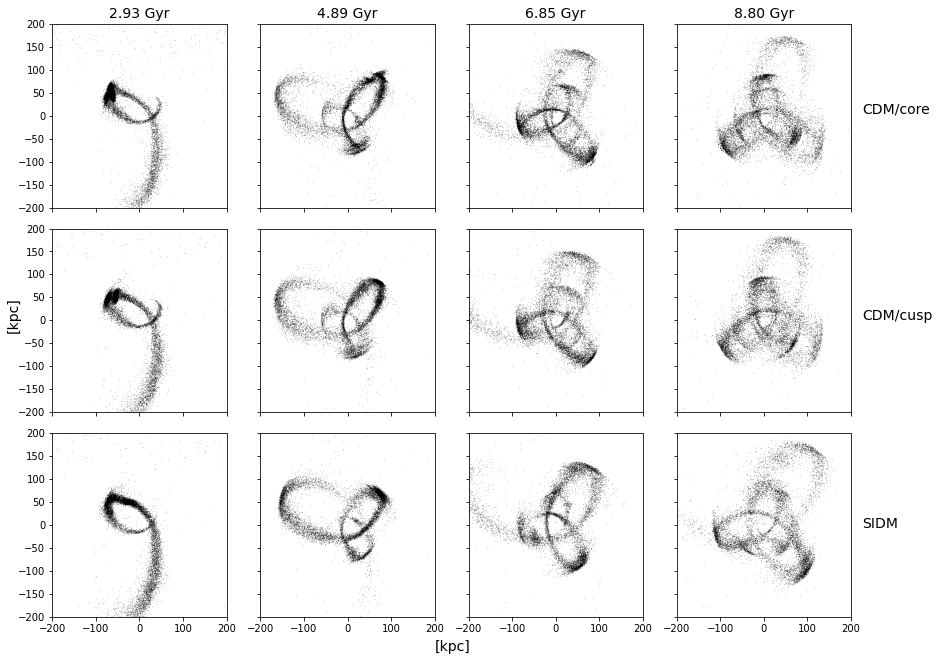
\includegraphics[width=0.9\linewidth]{figs/stars_bw.png}
    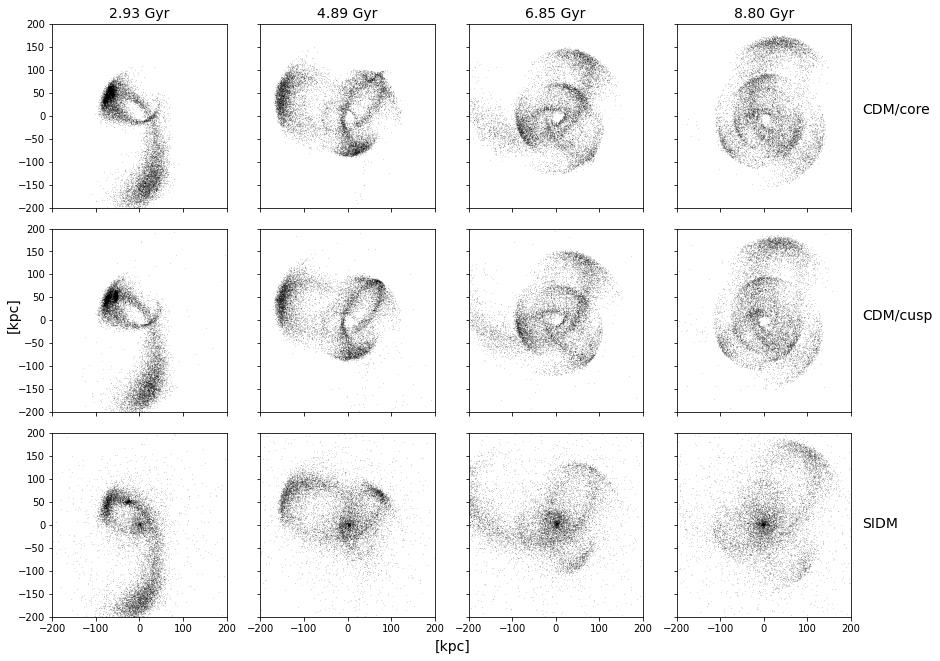
\includegraphics[width=0.9\linewidth]{figs/darks_bw.png}
    \caption{%
        Positions of Sgr stellar (top three rows) and dark matter (bottom
        three rows) particles at various times for all three of the considered
        mergers.  Each column denotes a different time; each row a different
        merger.
    }
    \label{fig:inits}
\end{figure}

Even from these plots, there are some interesting patterns to note. First, we
notice the development of a winding stream structure much like that reported
in~\cite{dierickx_predicted_2017} by around 6 to 7 Gyr in all three cases. We
can also note that the CDM/core and CDM/cusp streams are rather similar, with
the general shape, size, and overall rotation in agreement. There do exist some
differences particularly at later times, however, particular in the inner
stellar structure.  For example, at 6.85 Gyr, one can see a sharply defined
inner stream at $(20,60)$ kpc in the CDM/cusp stream which is significantly
fuzzier and less dense in the CDM/core case.  Similar differences emerge at
the later 8.80 Gyr time stamp.

There are much more marked differences between the SIDM and CDM cases,
however.  The stream arms appear to be slightly rotated clockwise relative to
the CDM mergers, and the general shape of the inner structure is very
different.  In particular, the CDM merger appear to show doubled-stream shape
for the inner arms at the later time stamps which is entirely non-existent in
the SIDM case.  These differences are even more apparent when looking at the
distribution of dark matter.  In the CDM mergers, the dark matter distribution
appears to roughly trace out the distribution of the stream and has a distinct
hole at the origin.  In the SIDM merger, however, the dark matter distribution
largely loses the precise shape of the stream, instead collapsing inward
toward the MW center.

We can also look at the density of particles in the orbital plane by performing
a two-dimensional histogram on the data in Figure~\ref{fig:inits}.  The result
is shown in Figure~\ref{fig:densities}.  The densities are integrated over the
axis perpendicular to the orbital plane.

\begin{figure}
    \centering
    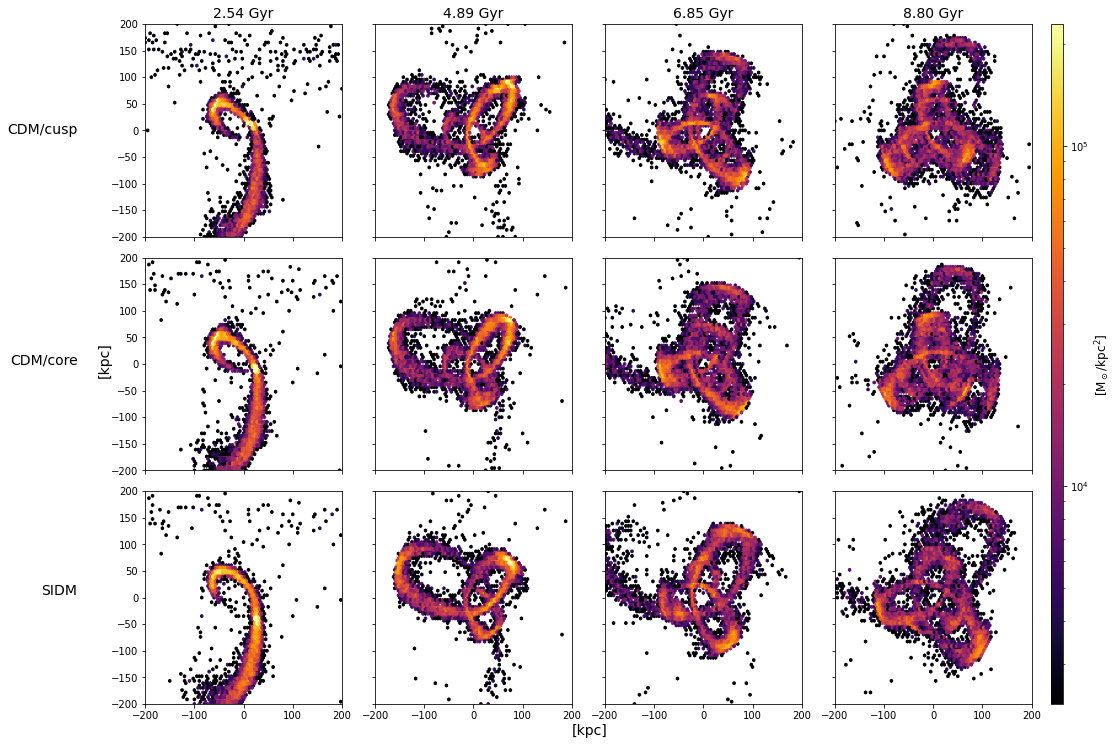
\includegraphics[width=0.9\linewidth]{figs/density_stars.png}
    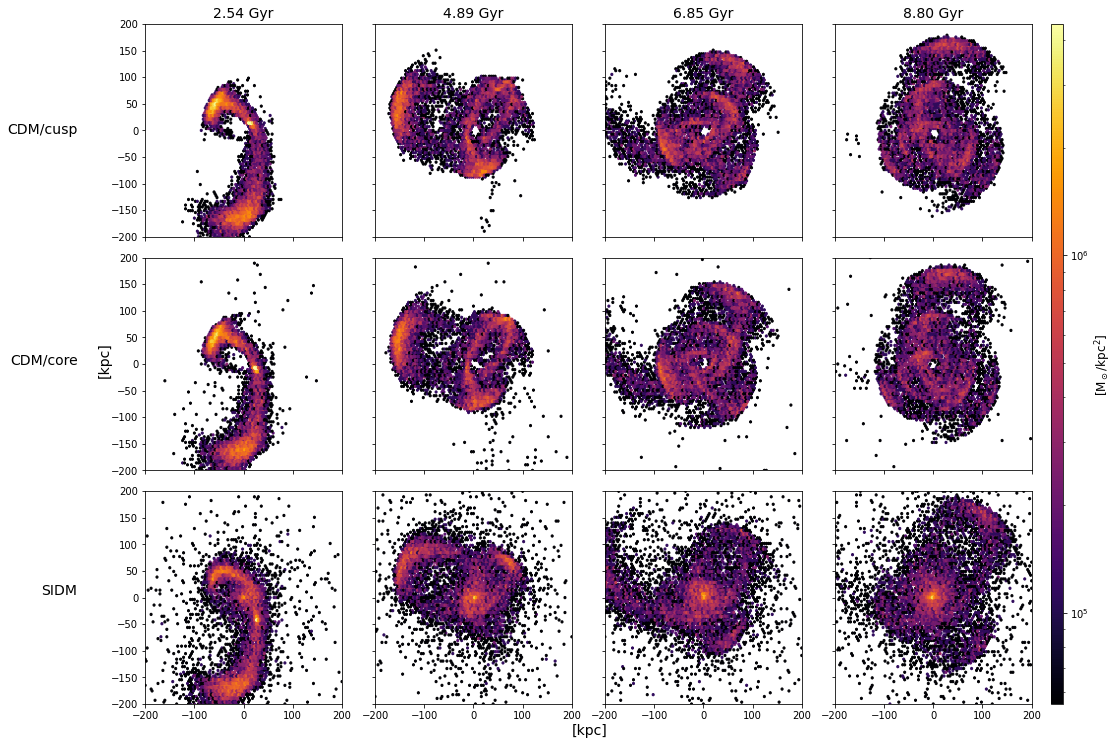
\includegraphics[width=0.9\linewidth]{figs/density_darks.png}
    \caption{%
        Two-dimensional density histogram of the stellar (top three rows) and
        dark matter (bottom three rows) Sgr particles at various times for
        each considered merger.  Densities are integrated over the axis
        perpendicular to the orbital plane.
    }
    \label{fig:densities}
\end{figure}

The density plots allow us to more strictly quantify some of the trends noted
previously. For example, the dark matter density plots show quite concretely
that the dark matter distribution in the SIDM case peaks at the Galactic center,
where there is a distinct hole in the CDM mergers. The SIDM particles are also
significantly less well-constrained, with a large spread extending beyond the
limits of the plot. This is compared to the CDM cases, where there are
relatively few particles outside of the path of the stream.

Looking at the density distribution of the stellar particles allows us to
quantify some of the differences noted earlier.  For example, at 6.85 Gyr, the
SIDM stream has a relatively high-density ($\sim 10^5$ M$_\odot$/kpc$^2$)
stream arc extending from approximately $(-20,0)$ kpc up to around $(60,125)$
kpc.  The corresponding arc exists in the CDM cases, but it is less
well-defined (there is more horizontal spread) and lower density ($\sim 10^4$
M$_\odot$/kpc$^2$).

There are other, similar differences, but we would do better to analyze these
differences for the specific time stamps of each merger which most closely
approximate Sgr today. Determining this requires mapping the position of the Sgr
progenitor, however.


\hypertarget{identifying-the-sgr-progenitor}{%
\section{Identifying the Sgr
progenitor}\label{identifying-the-sgr-progenitor}}

A key part of analyzing these data is to understand the trajectory and
evolution of the Sgr progenitor.  As such, we desire a method for successfully
identifying the position of the Sgr progenitor throughout its evolution.  This
is less straightforward than it may sound because of the strong effects of
tidal stripping.  These mean that we need to identify which particles are
stripped or bound to the progenitor at any given point and omit stripped
particles from our calculation of the progenitor position.  In our tests, we
tried a few different methods which we will describe here.

The first method that we tried was to track bound versus unbound star
particles by counting particles as stripped once they exceeded a fixed radius
from the center of mass of bound particles.  The algorithm for this is as
follows.  We begin by counting the stellar particles within a certain radius
on the first snapshot to be ``bound''.  For each snapshot after, we find the
center of mass of the bound particles.  Then, for each bound particle, we
compute its distance from the center of mass.  If this exceeds the fixed
stripping radius, we unmark the star as bound and continue.

As stated, this algorithm has two parameters that can be tuned: the initial
stripping radius for the initial Sgr stellar positions and the fixed stripping
radius for all following snapshots.  We found it useful to describe the
initial stripping radius instead in terms of the percentage of particles that
are initially counted as ``bound''.  For example, we say that the we start
with the innermost 20\% of particles and proceed with a fixed radius of 20
kpc.  The results of applying this algorithm to the CDM/cusp merger data with
a few different choices of parameters can be seen in
Figure~\ref{fig:fixed_star}.

\begin{figure}
    \centering
    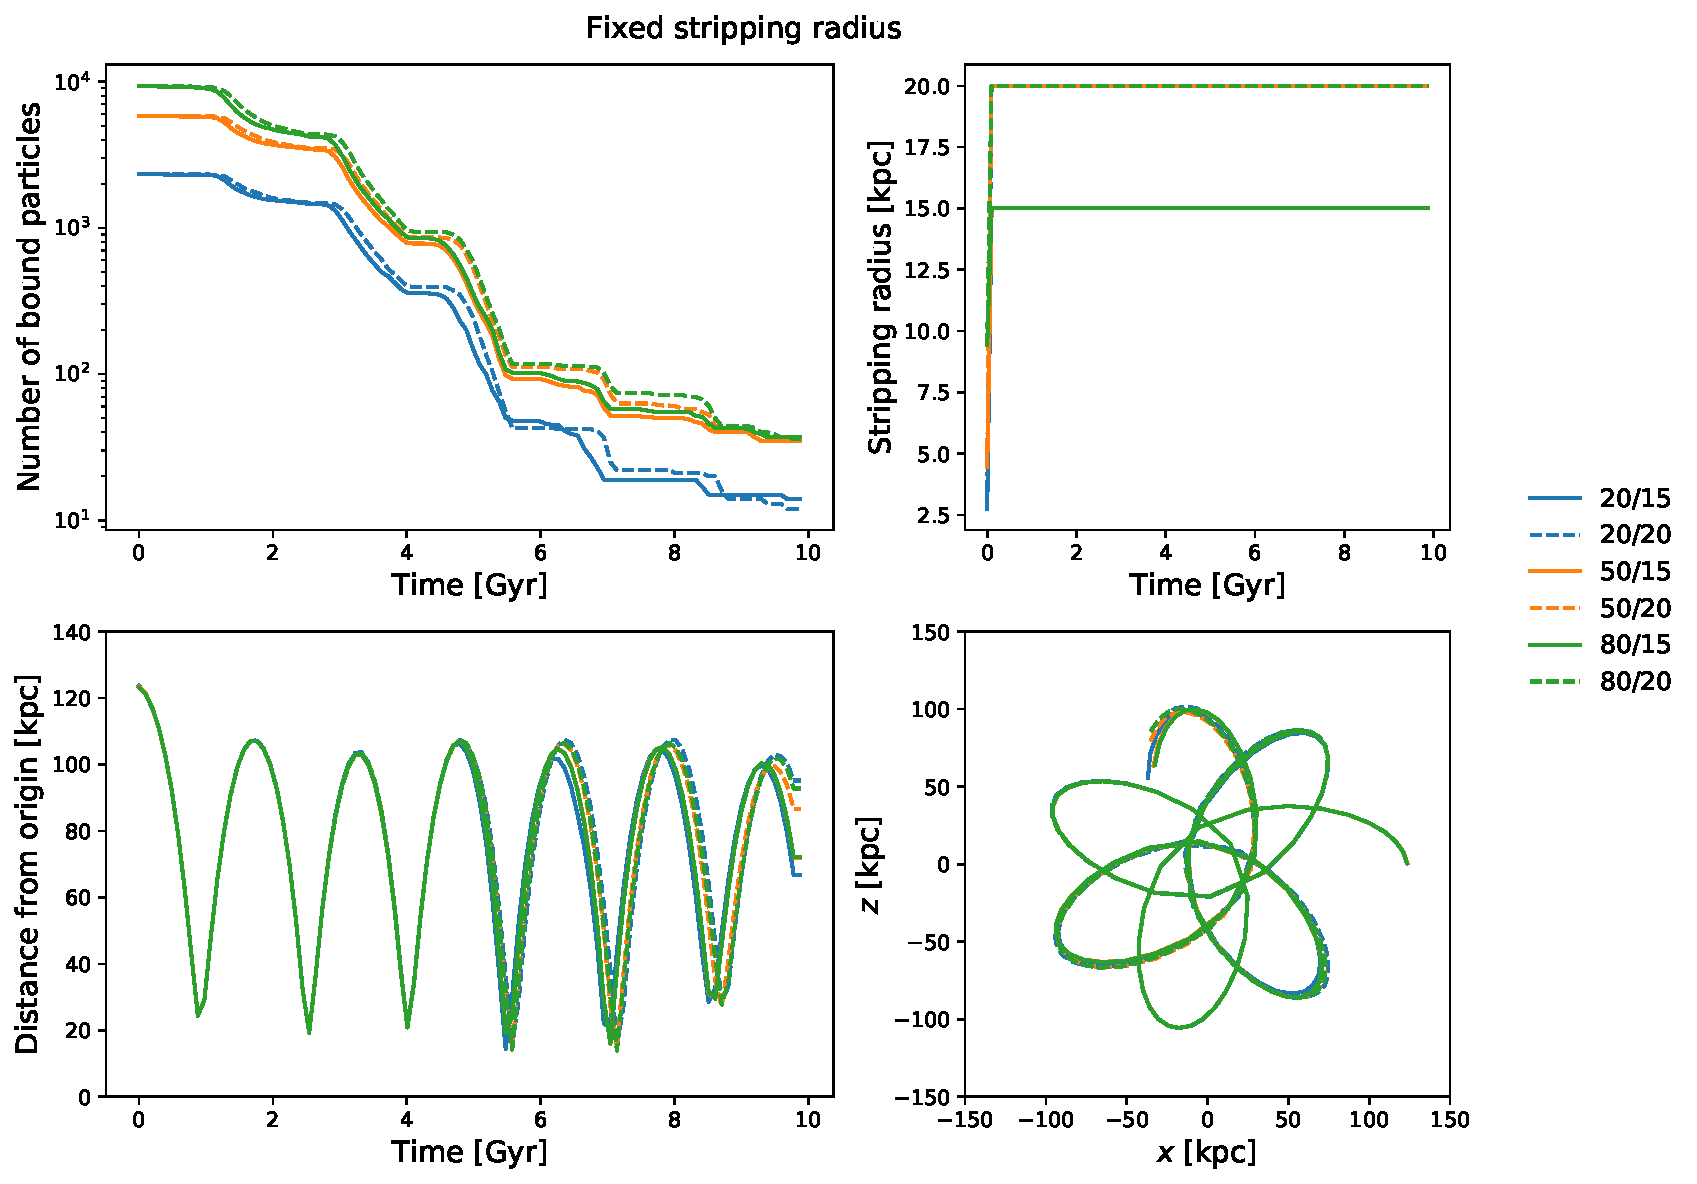
\includegraphics[width=0.9\linewidth]{figs/fixed_star.pdf}
    \caption{%
        Results of applying the ``fixed stripping radius''
        progenitor-identifying algorithm to the CDM/cusp merger data. Entries in
        the legend are given in the following format: ``a/b'' means that we
        started with the innermost ``a''\% of stellar particles and proceeded
        with a fixed stripping radius of ``b'' kpc.  In the upper left is the
        number of bound particles over time.  The upper right shows the
        stripping radius.  The bottom left shows the distance from the origin
        to the Sgr center of mass; an estimate of the MW-Sgr separation.  The
        bottom right shows the trajectory of the progenitor in the orbital
        plane.
    }
    \label{fig:fixed_star}
\end{figure}

This figure shows us that starting with too few of the initial particles (in
this case, 20\%) leads to very small numbers of bound particles at late times.
Further, it shows us that the trajectory of the progenitor can be somewhat
sensitive to the chosen algorithm parameters, especially at late times.

This algorithm appears to have two issues that we want to try to solve.
First, the actual size of the progenitor is expected to shrink with time, as
progressively more of the particles are stripped.  By using a fixed stripping
radius, we are not modeling the expected decay of the progenitor size.  The
second problem we encountered is that this method appears to leave us with
only $\mathcal{O}(10)$ bound particles after around 6 Gyr evolved.  As such,
we decided to explore modifications to the algorithm.

The first modification was to consider a decreasing stripping radius.  The
algorithm is very similar to before.  On the first snapshot, we count some
inner fraction of the particles to be ``bound'' and find the radius of this
ball of bound particles.  For the next snapshot, we strip any particles
which exceed this radius (times a constant).  \textit{However}, after
stripping away particles, we recompute the radius of the ball of the bound
particles, and reset the stripping radius equal to this. For each snapshot
following, we strip particles that are beyond this radius and recompute the
radius.  Over time, the stripping radius will decrease, modeling the
progressively decreasing size of the progenitor.  Some basic tests showed that
this algorithm often becomes a bit too aggressive, so we introduced a minimum
stripping radius, such that the algorithm would never use too small a stripping
radius. 

Further testing with a minimum stripping radius of 8 kpc and a variety of
different initial parameters showed the algorithm to simply be too aggressive.
For all considered combinations of parameters, we found that the algorithm
reduced itself below the minimum stripping radius by around 6 Gyr.  This means
that at later times, when we might expect the closest resemblance to the
observed Sgr progenitor, the algorithm reduces to the fixed stripping radius
algorithm with a fixed radius of 8 kpc. 

One possible reason that it becomes too aggressive is because the actual
size of the progenitor is not monitonically decreasing.  Rather, its size
fluctuates over the course of the orbit, becoming quite compressed and small
near the pericenter and a bit more spread out and large near the apocenter.
These effects are modeled by the King formula for the tidal
radius~\cite{king_structure_1962} as given in~\cite{dierickx_predicted_2017}:
\begin{equation} \label{eq:king_radius}
    r_t = r \left[ \frac{1}{2} 
    \frac{M_{\text{Sgr}}(<r_t)}{M_{\text{MW}}(<r)} \right]^{1/3},
\end{equation}
where $M_{\text{gal}}(<r)$ is the enclosed halo mass in galaxy ``gal'' within
radius $r$ of the center of mass of the galaxy, $r$ is the distance between
the Milky Way and Sgr centers of mass, and $r_t$ is the tidal radius.  For a
given snapshot, then, we can compute the tidal radius according to this
formula by subtracting $r_t$ from both sides and using a simple root finder to
identify the $r_t$ which solves the equation.  We then strip any particles
which are farther than $r_t$ away from the center of mass of the progenitor at
the current time.  Again, initial testing showed that this algorithm needed a
minimum stripping radius to prevent it from stripping away all the stellar
particles.

Further testing with a minimum stripping radius of 8 kpc showed this algorithm
to also be too aggressive.  We tried to add a multiplicative factor to the tidal
radius in order to make it a little larger before stripping, but this did not
appear to help very much. After only a few Gyr, this too reduced effectively to
the fixed radius strategy, using only the minimum stripping radius.

At this point, we concluded that the issue of too few bound particles at late
times may be a problem related to our relatively small number of Sgr stellar
particles, instead of a problem with the algorithms themselves.  As such, we
decided to try to use the fixed radius algorithm but using both stellar
\textit{and} dark matter particles.  The result on the CDM/cusp data is shown
in Figure~\ref{fig:fixed_both}.

\begin{figure}
    \centering
    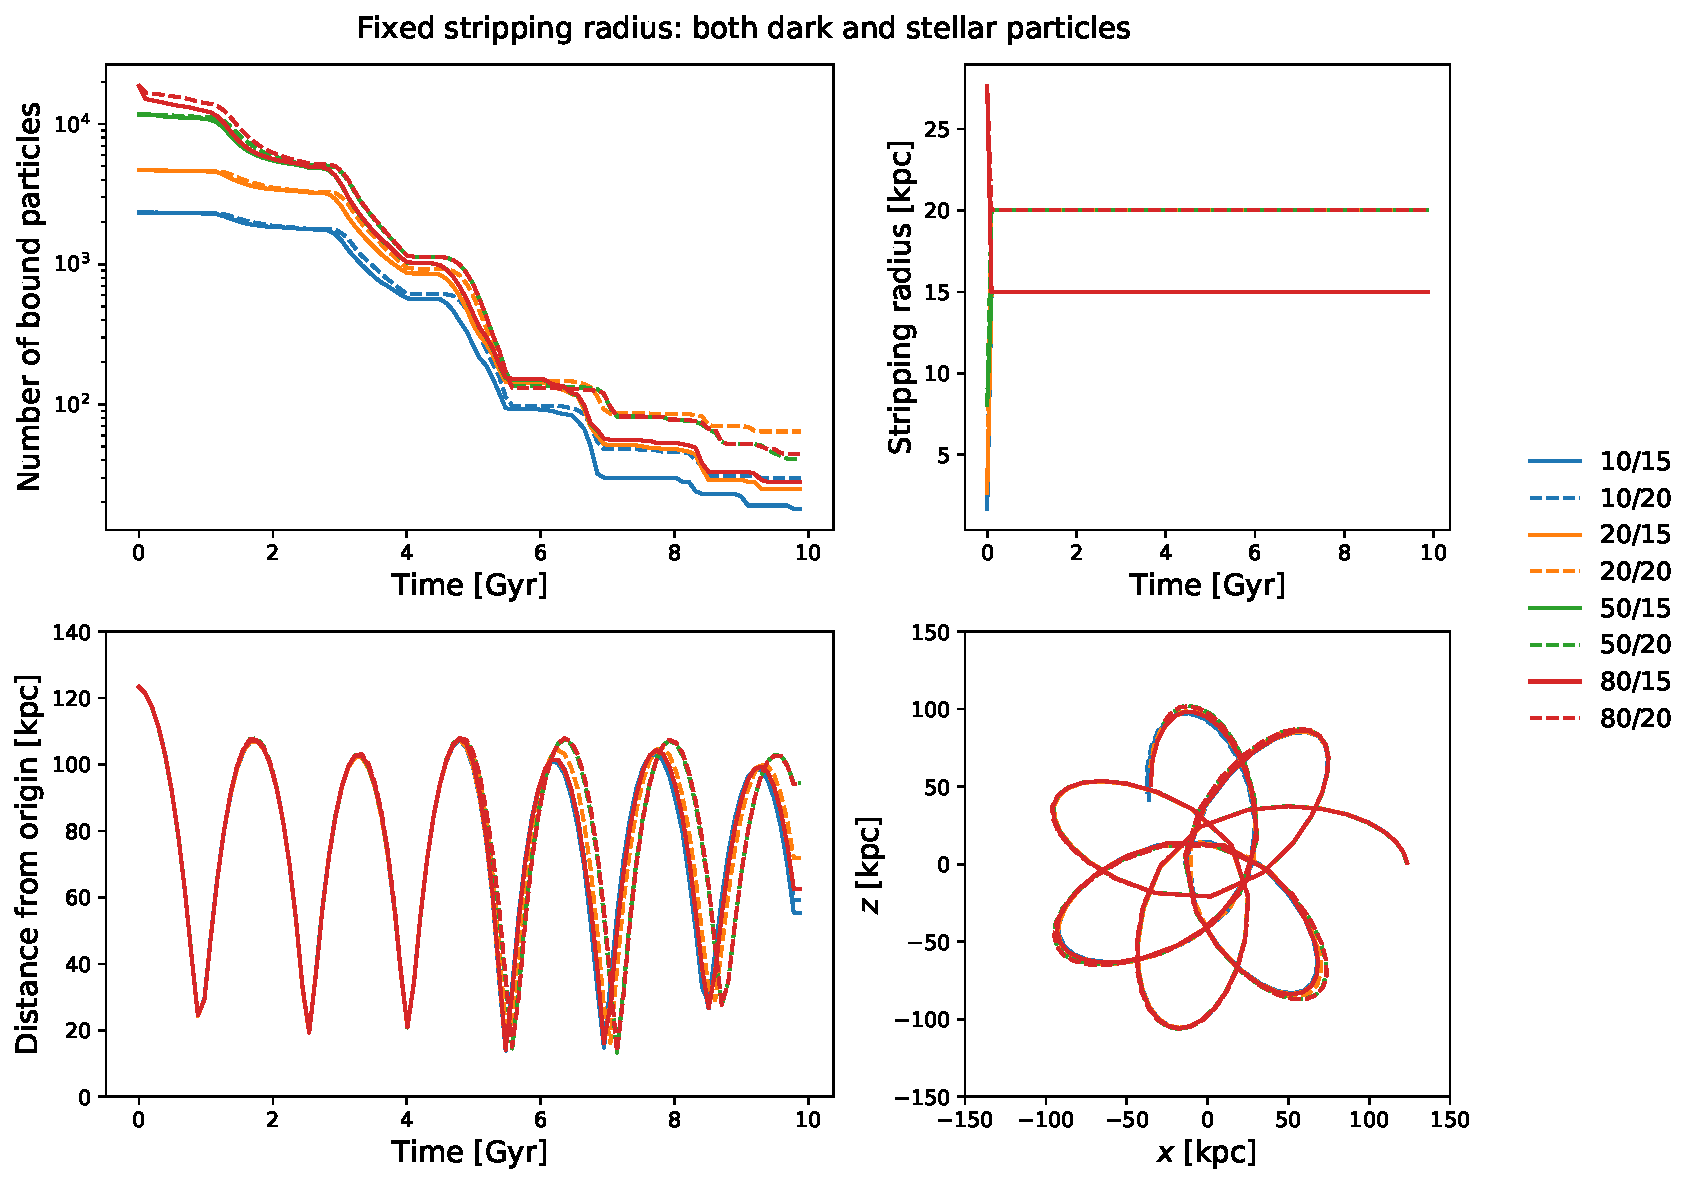
\includegraphics[width=0.9\linewidth]{figs/fixed_both.pdf}
    \caption{%
        Results of using the ``fixed stripping radius'' progenitor-identifying
        algorithm on all the particles in the CDM/cusp merger data. Plots and
        legend entries have the same meaning as in
        Figure~\ref{fig:fixed_star}.
    }
    \label{fig:fixed_both}
\end{figure}

This appears to yield promising results. We note that there are generally more
``bound'' particles at late times when using all particles than when only using
stellar ones, and that, aside from the ``50/20'' and ``80/20'' runs, the
resulting trajectories appear to be more robust to the algorithm parameters. As
such, we choose to move forward with this algorithm using the ``20/20''
parameters, as they appear to be consistent with the majority of the other
parameter choices and yield the most bound particles in the end. Using these
choices to identify the progenitor, we apply the algorithm to all three mergers.
The resulting data are shown in Figure~\ref{fig:all}.

\begin{figure}
    \centering
    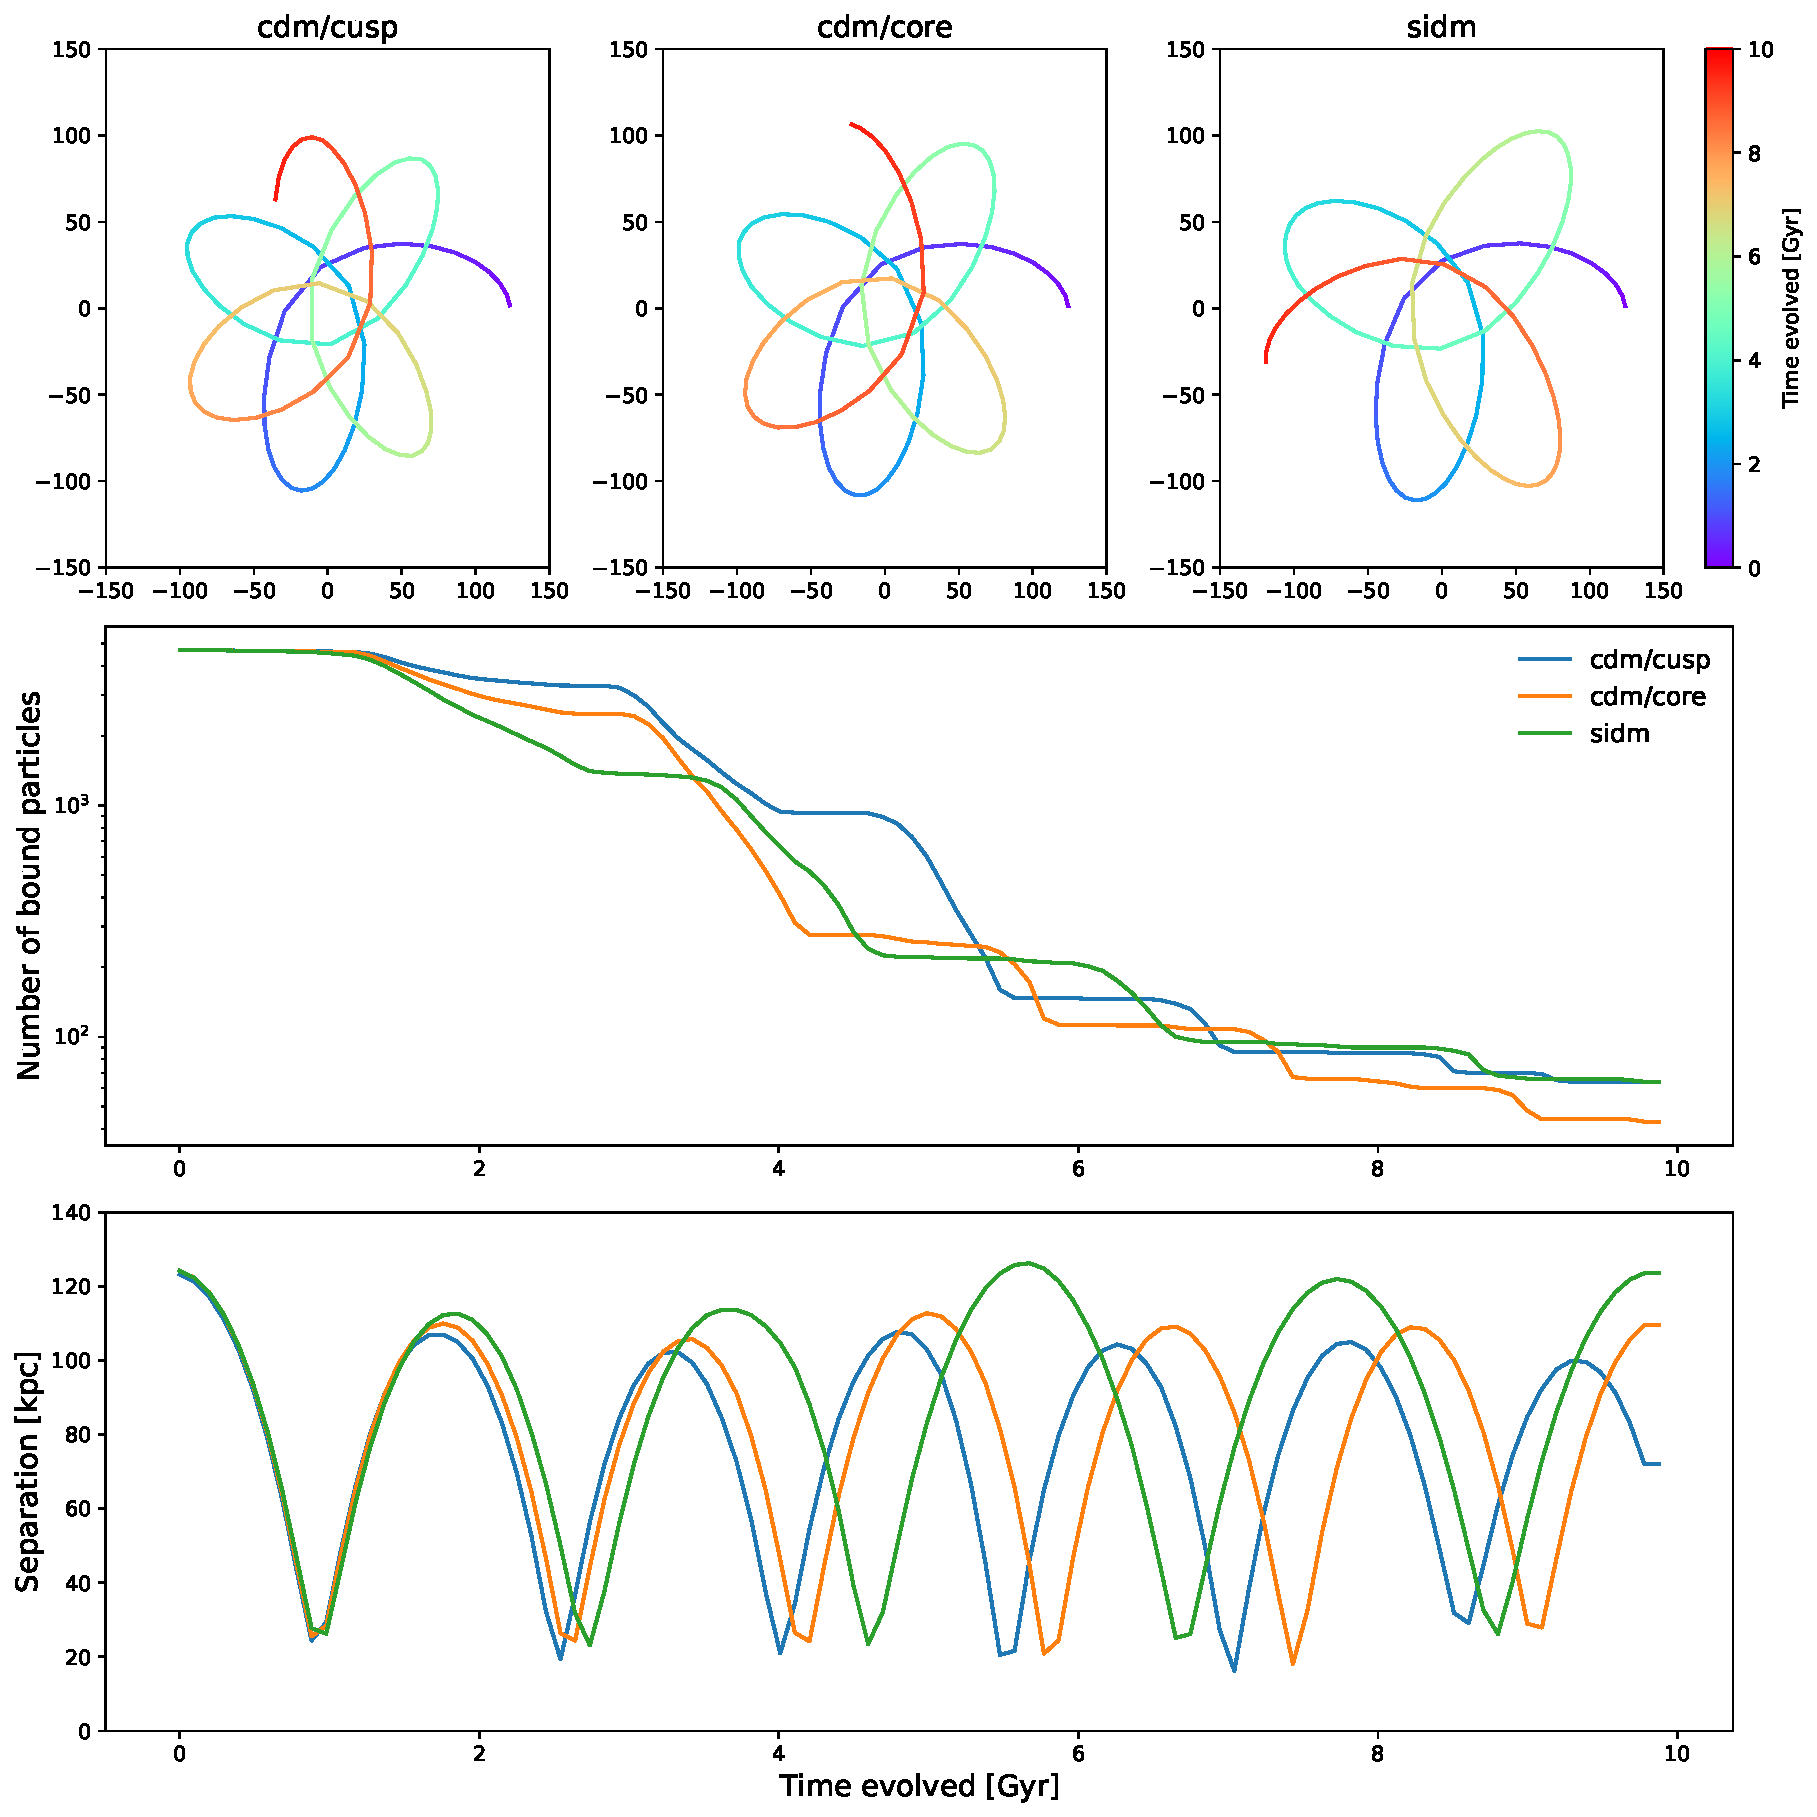
\includegraphics[width=0.9\linewidth]{figs/all_mergers_pretty.pdf}
    \caption{%
        Results of using the ``fixed stripping radius'' progenitor-identifying
        algorithm on all the particles in each of the mergers. We use the
        ``20/20'' algorithm parameters for all mergers, meaning that we start
        with the inner 20\% of particles and use a 20 kpc stripping radius. The
        top row shows the trajectory of the Sgr progenitor in the orbital plane
        for each merger. The middle row plot shows the number of bound particles
        over time. The bottom row plot shows the MW-Sgr separation over time.
    }
    \label{fig:all}
\end{figure}

The plots in this figure are evidence that SIDM microphysics may indeed have a
profound impact on the resulting trajectory of the Sgr satellite.  One such
difference is that the number of bound particles decreases much more
substantially at early times than either of the two CDM runs.  This could be
explained by considering that self-interactions provide a mechanism for dark
matter to free itself from shallow gravitational potential wells to which
collisionless dark matter would remain confined.

Looking at the MW-Sgr separation over time, it is immediately evident that the
cored profile yields a slightly longer orbital period, given the slowly
increasing distance between the apo- and pericenters of the CDM/cusp and
CDM/core orbits.  The inclusion of self-interactions appears to add to this
effect, with the CDM/cusp progenitor attaining six pericenters before the SIDM
orbit is able to reach a fifth.

One phenomenon showcased by the separation curves which is difficult to
understand is the lack of a consistent decay in the apocenters.  We compare to
Figure 6 of~\cite{dierickx_predicted_2017}, which shows a steadily decreasing
apocenter.  This is the expected behavior; as the Sgr progenitor orbits and
decays, we would expect it to lose energy and steadily fall inward.  This,
however, does not appear in our plots.  In fact, this phenomenon is
exacerbated in the SIDM merger, where the apocenter actually appears to
\textit{grow} after around 4 Gyr, reaching nearly 130 kpc at the 6 Gyr mark.
The mechanism by which this would occur is not yet understood.

Future studies would do well to explore other algorithms for identifying the Sgr
progenitor, such as a friends-of-friends (FOF) halo-finder. These difficulties
would also likely be alleviated by greater stellar resolution through the use of
more stellar particles and the inclusion of a stellar bulge. 


\hypertarget{comparison-to-stream-data}{%
\section{Comparison to stream data}\label{comparison-to-stream-data}}

\hypertarget{progenitor-coordinates}{%
\subsection{Progenitor coordinates}\label{progenitor-coordinates}}

As stated previously, a description of the orbit of the progenitor will allow us
to determine the specific time stamps at which our mergers most closely
approximate Sgr today.  We take the observed coordinates of Sgr to be
$(\alpha, \delta) = (283.83, -29.45)$ degrees (where $\alpha$ is right
ascension and $\delta$ is declination)~\cite{nasa_nasaipac_nodate}, proper
motion $(\mu_\alpha \cos\delta, \mu_\delta) = (-2.54 \pm 0.18, -1.19 \pm
0.16)$ mas/yr~\cite{massari_hubble_2013}, heliocentric distance $24.8 \pm 0.8$
kpc~\cite{kunder_distance_2009}, and line-of-sight velocity $179 \pm 1$
km/s~\cite{dierickx_predicted_2017,bellazzini_nucleus_2008}.  

To compare our data to these coordinates, we must convert from Galactocentric
distances in the orbital plane to equatorial coordinates.  We do this using the
Astropy package~\cite{astropy_collaboration_astropy_2013,
astropy_collaboration_astropy_2018} with the assumptions that the Sun is
located at approximately $(8,0,0)$ kpc with a velocity which is approximately
directed in the positive $y$ direction.  The resulting coordinates over time
are shown in Figure~\ref{fig:eq_prog}.  We note that the right ascension data
generally moves from left to right across the plot and is meant to be
interpreted as wrapping around from the right edge back to the left.

\begin{figure}
    \centering
    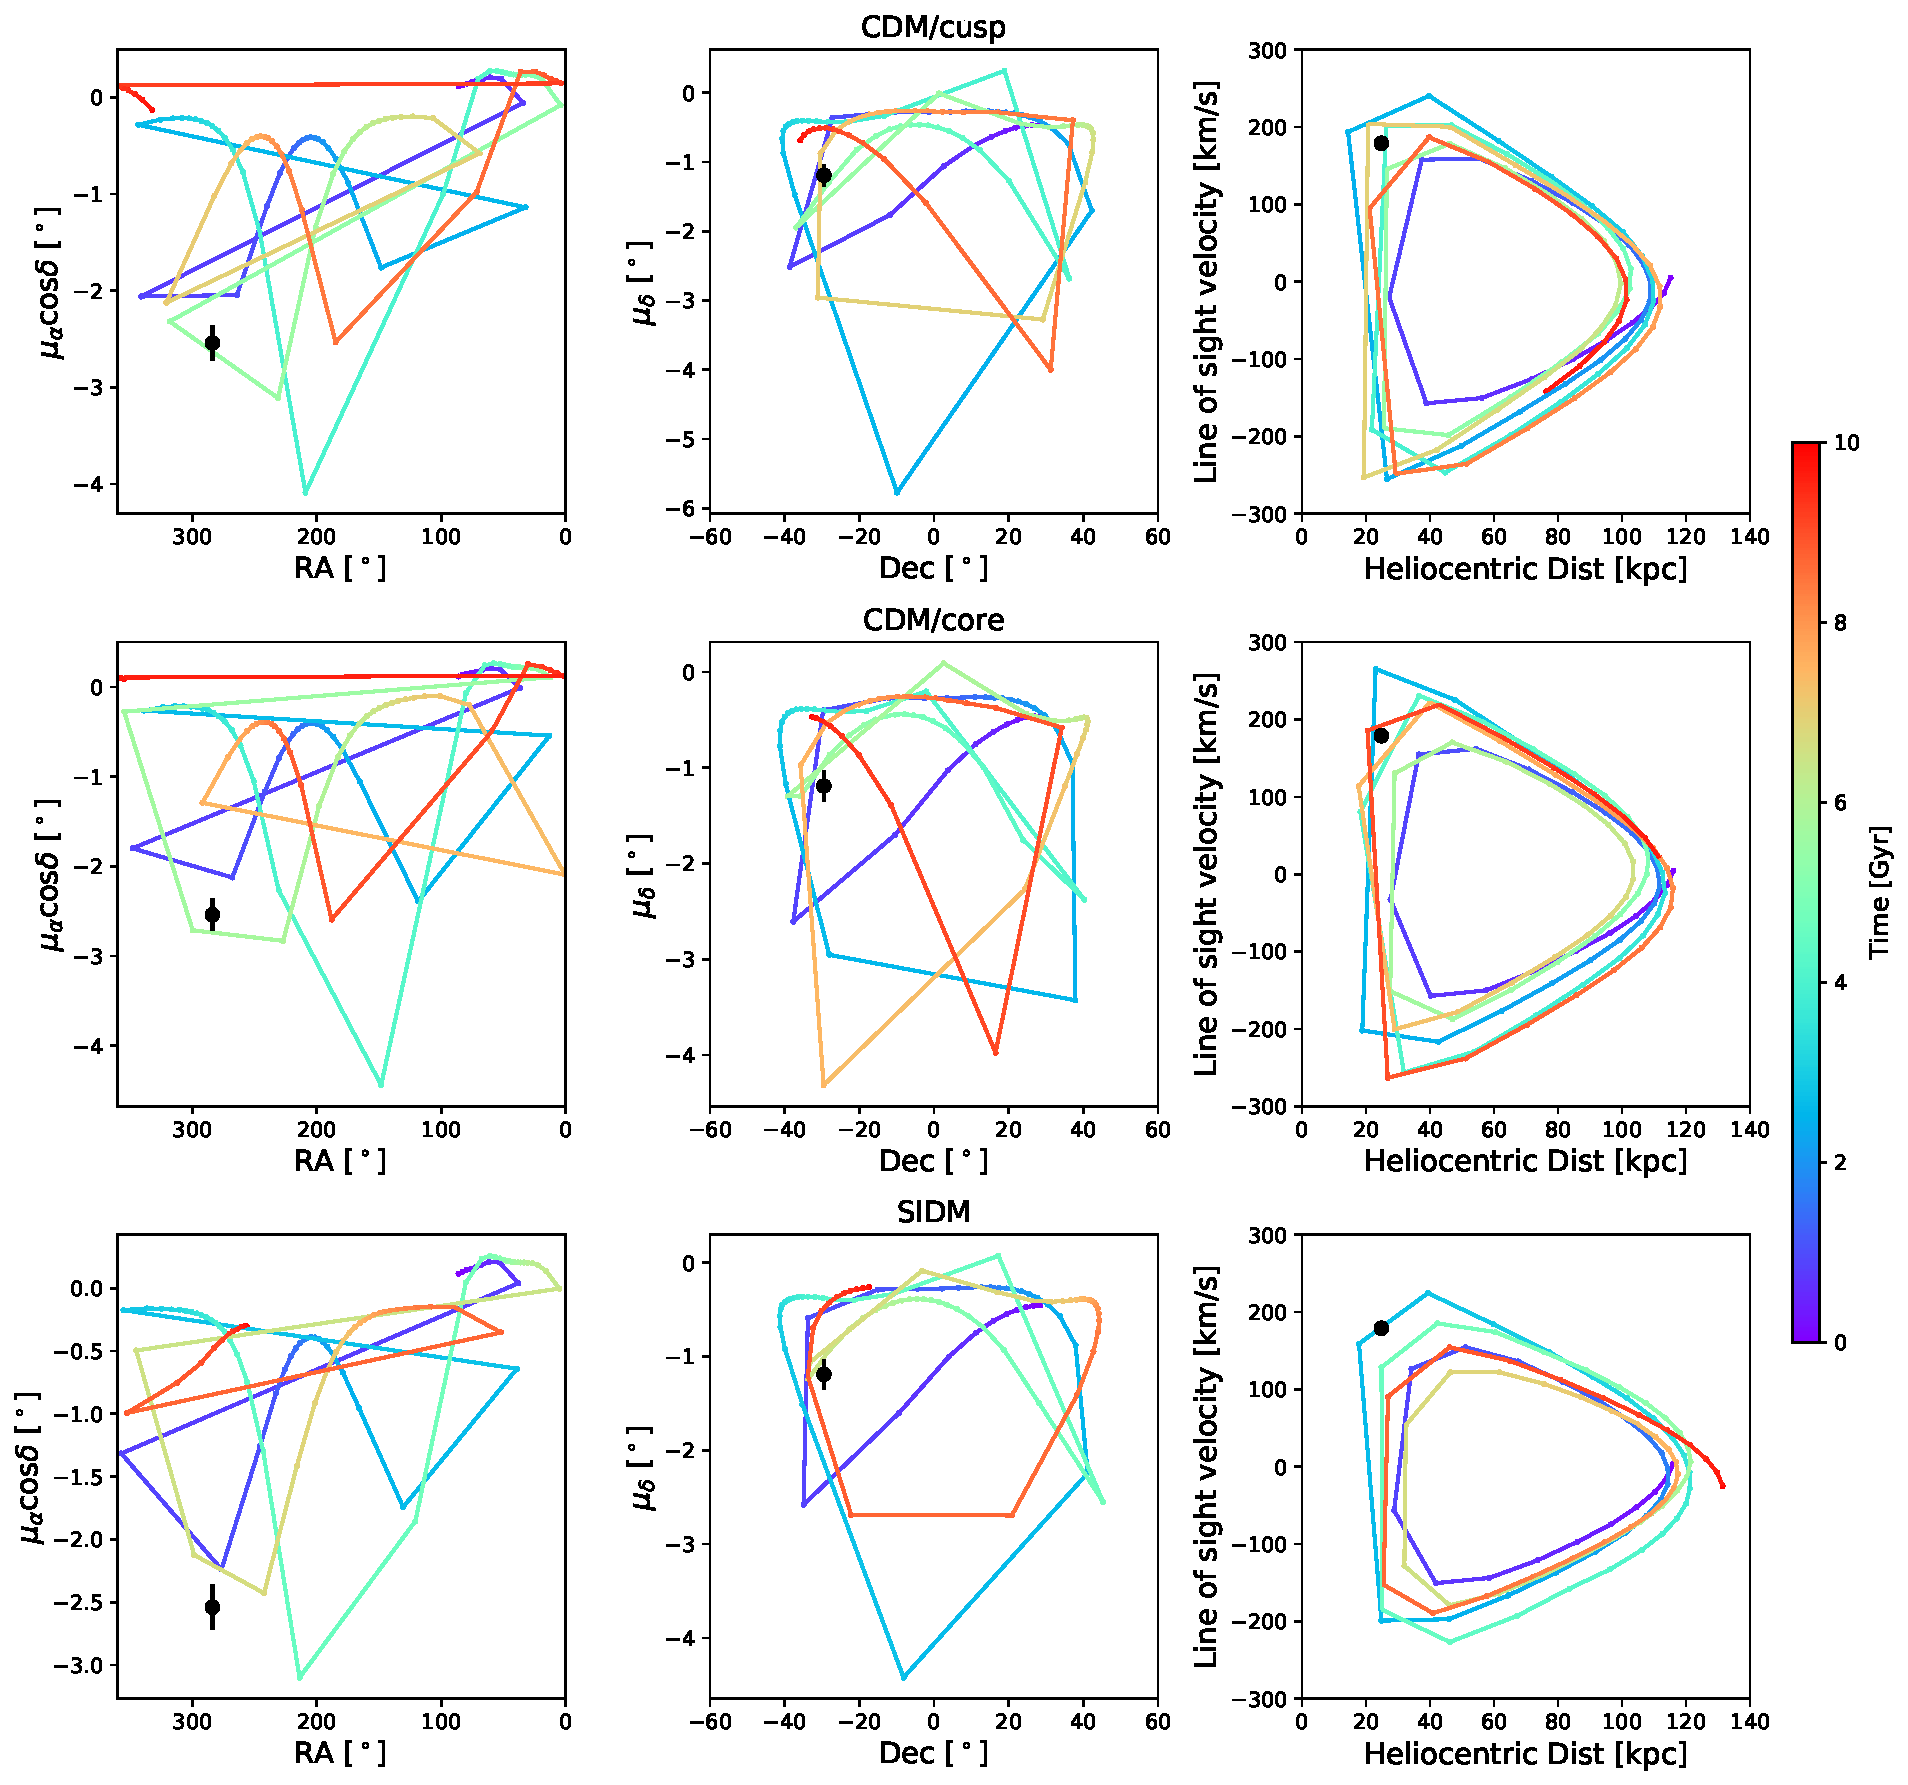
\includegraphics[width=1.0\linewidth]{figs/equatorial_progenitor.pdf}
    \caption{%
        Trajectory of the Sgr progenitor in terms of equatorial coordinates and
        proper motions for each merger. Black squares represent the observed
        coordinates of the progenitor today. Error bars are present for observed
        quantities with uncertainties, though are in some cases smaller than
        the size of the marker (particularly in the velocity versus distance
        subplots).
    }
    \label{fig:eq_prog}
\end{figure}

We note that the Dierickx 2017 model~\cite{dierickx_predicted_2017} most
closely approximated the observed coordinates just after its fifth pericenter,
with the best agreement with the stream shape occurring then as well.
Unfortunately, no snapshot of our model comes as close to these coordinates as
theirs, but we believe that this discrepancy would be alleviated somewhat by
greater time resolution in the snapshots of the stream.  We do, however, find
that the CDM mergers attain their closest matches to the observed coordinates
just after their fifth pericenters (approximately 7.04 Gyr and 7.43 Gyr for
the /cusp and /core cases, respectively), in accord with the Dierickx model.
The SIDM merger attains its closest match after its fourth pericenter
(approximately 6.75 Gyr) with its fifth pericenter (approximately 8.80 Gyr)
the next closest match.

In particular, the line-of-sight velocity versus heliocentric distance plots
in the Figure show a curious trend.  In the CDM cases, the trajectory passes
roughly through the observed velocity and distance with every pericentric
passage except the first.  By contrast, no time stamp of the SIDM merger after
the third pericenter appears to closely replicate the observed velocity.  At
such early times, however, Sgr has not completed enough wraps for the resulting
stream to match existing models, such as Law 2010 or Dierickx 2017.  We also
note that the orbital period of the SIDM merger was seen to be significantly
longer than that of either CDM merger; we believe this to be consistent with
the smaller line-of-sight velocities observed here.

We can also use our progenitor-identifying algorithm to obtain estimates of the
times at which each stellar particle comes unbound from the progenitor. We can
thus look at the line-of-sight velocity and heliocentric distance for each star
of the mergers at their respective fifth pericenters, colored according to their
stripping time.  Note that any particles which are still bound at the time of
the snapshot are colored black.  We choose to use the fifth pericenter for the
SIDM merger as well because it gives the best agreement with the observed
distance and line-of-sight velocity at late times, despite poorer agreement
with the other dimensions.  This is shown in Figure~\ref{fig:vel_v_dist}.

\begin{figure}
    \centering
    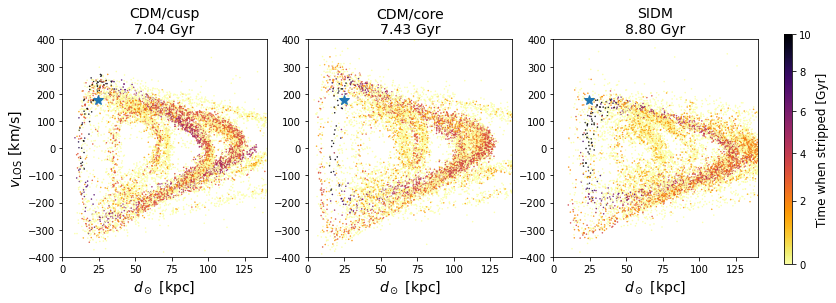
\includegraphics[width=1.0\linewidth]{figs/vel_v_dist_peri_only.png}
    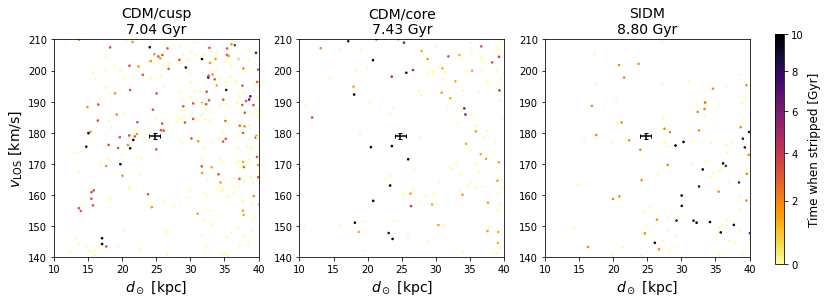
\includegraphics[width=1.0\linewidth]{figs/vel_v_dist_zoomed.png}
    \caption{%
        Line-of-sight velocity versus heliocentric distance for Sgr stellar
        particles in each merger, colored according to the time at which each
        particle became unbound from the progenitor. Each merger is given at its
        fifth pericenter. (Top) The full spread of Sgr stellar particles closer
        than 140 kpc, with the observed coordinates shown as a blue star.
        (Bottom) Only the Sgr stellar particles which are close to the observed
        coordinates; observed coordinates denoted by black error bars.
    }
    \label{fig:vel_v_dist}
\end{figure}

The resulting Figure gives a strong indication that the simulated SIDM
progenitor is indeed unable to adequately reproduce the observed line-of-sight
velocity of Sgr.  In particular, we note that both CDM mergers display a
number of bound (colored dark) particles which roughly surround the observed
coordinates.  The SIDM merger, however, shows that all bound particles either
have too small a line-of-sight velocity or too large a heliocentric distance
to yield the observed progenitor coordinates.  We note further that this
discrepancy is very significant with respect to the uncertainties in the
measured coordinates.


\hypertarget{stream-shape}{%
\subsection{Stream shape}\label{stream-shape}}

The next piece of the analysis that we will consider is a comparison to data
from the second data release (DR2) of the \textit{Gaia}
mission~\cite{lindegren_gaia_2018,gaia_collaboration_gaia_2018}, from which Sgr
stars have been identified by Ibata et al.~\cite{ibata_panoramic_2020} using the
\verb|STREAMFINDER| (hereafter \verb|SF|)
algorithm~\cite{malhan_streamfinder_2018, malhan_ghostly_2018}.  The resulting
dataset includes the \textit{Gaia} equatorial coordinates, proper motions,
magnitudes, and colors of 263,438 stars, along with an estimate of the
distance provided by the algorithm.  They find their dataset to agree well
with the Law 2010 model~\cite{law_sagittarius_2010}, barring a few small
deviations.  The \verb|SF| sample is shown in equatorial coordinates in
Figure~\ref{fig:streamfinder}.  We note in particular a very dense region of
stars at around $\alpha = 280^\circ$, $\delta = -30^\circ$, and heliocentric
distance $\approx 30$ kpc.  This is the Sagittarius progenitor.

\begin{figure}
    \centering 
    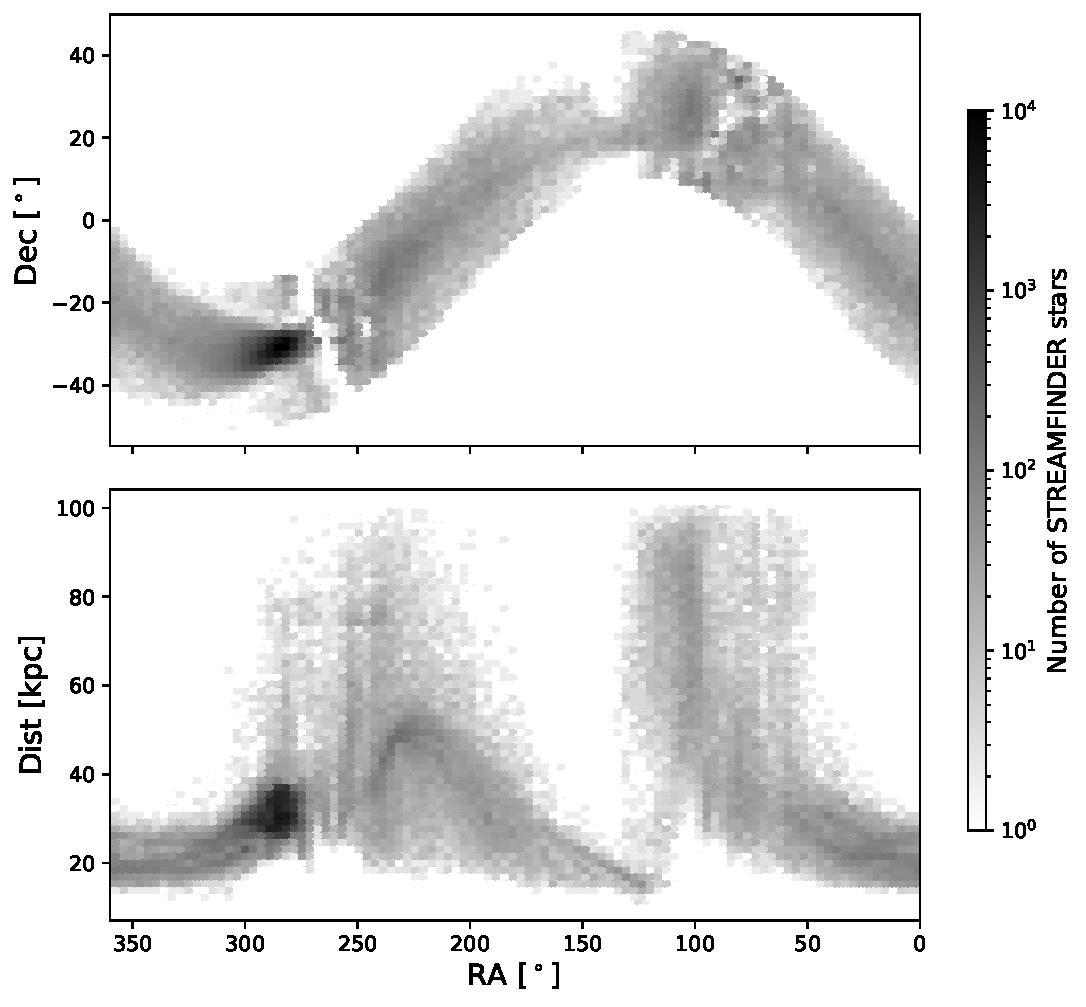
\includegraphics[width=0.7\linewidth]{figs/streamfinder.pdf}
    \caption{%
        Equatorial coordinates and estimated heliocentric distances for the
        263,438 Sgr stars identified by the \texttt{STREAMFINDER} algorithm.
    }
    \label{fig:streamfinder}
\end{figure}

For each merger, we continue to consider the fifth pericenter as before. We
again convert to equatorial coordinates, this time using only those stars with a
heliocentric distance less than 100 kpc, as the \verb|SF| sample
contains no stars beyond this threshold. The resulting distribution of stars is
plotted in Figure~\ref{fig:equatorial} with the \verb|SF| density
shown in gray.

\begin{figure}
    \centering 
    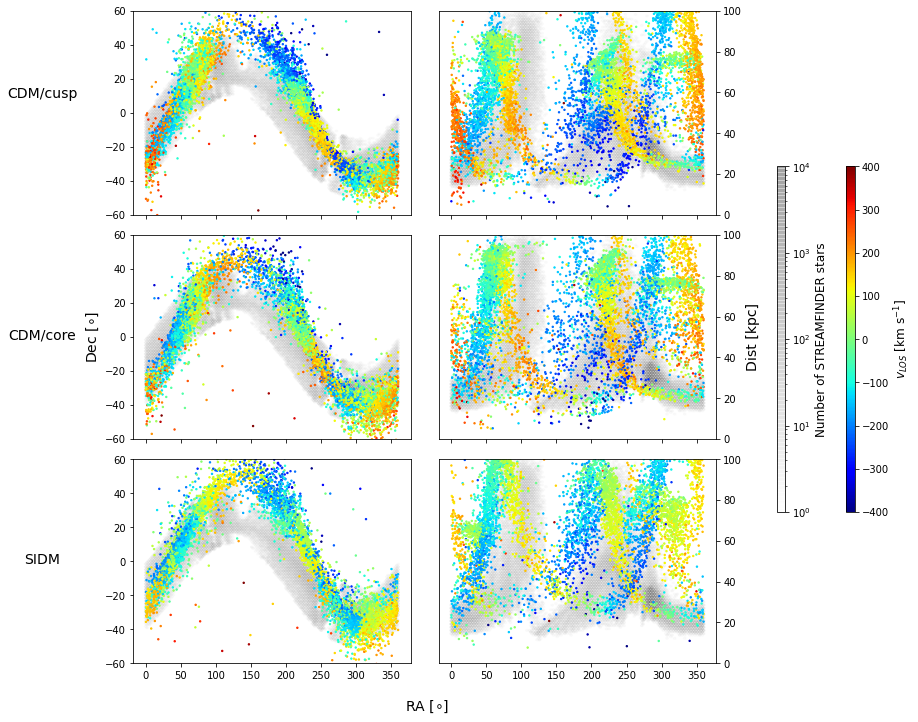
\includegraphics[width=1.0\linewidth]{figs/equatorial_streamfinder.png}
    \caption{%
        Equatorial coordinates for our simulated Sgr stellar particles of
        distances less than 100 kpc at the time of the fifth pericenter for
        each merger, colored by line-of-sight velocity.  The position of the
        simulated progenitor is shown by a white circle with black outline.
        (Note that it is located at RA $\approx 0.5^\circ$ in the CDM/core
        plots.) The observed coordinates of Sgr are shown as a black circle.
        The density of \texttt{STREAMFINDER} stars is shown in gray.
    }
    \label{fig:equatorial}
\end{figure}

Our comparison to the \verb|SF| stars shows qualitatively good agreement in
terms of the right ascension and declination, as the simulated streams appear
to reach their maximum and minimum values of declination at the same right
ascensions as the \verb|SF| stream.  We note that our streams are less thick
in most areas, perhaps owing to a smaller number of stellar particles.  Our
streams also reach a greater maximum declination than the \verb|SF| data; this
discrepancy appears to impact the CDM/cusp merger the least and the SIDM
merger the most.  The SIDM merger in general appears to have larger
declination values than expected from data.

When looking at the distribution of heliocentric distances, we note relatively
good agreement for right ascensions larger than $200^\circ$ in the CDM cases.
For smaller right ascensions, we do see the reproduction of the stream arm, but
shifted slightly toward larger right ascensions. This effect appears to be
less present in the CDM/core case. The SIDM merger also appears to reproduce the
stream arm for smaller right ascension, but is substantially less accurate at
reproducing that of larger right ascensions, with the whole of the stream
appearing to be shifted up by roughly $60^\circ$. The heliocentric distance
distribution also shows the predicted extensions to the leading and trailing
stream arms from the Dierickx model. 

When plotted in these coordinates, we can also discern some differences between
the mergers themselves. As an example, we can again see a marked difference in
the distribution of line-of-sight velocities, as the CDM mergers both show a
rather significant number of stars with large, positive line-of-sight
velocities (in the orange-red region of the colormap). The SIDM merger, by
contrast, has very few such stars, preferring smaller velocities. Unfortunately,
the \verb|SF| dataset does not come with radial velocities; as such, we choose
to use another dataset for this comparison.


\hypertarget{twomass}{%
\subsection{2MASS M-giants}\label{twomass}}

The final comparison we will make is with M-giant stars from the Two Micron All
Sky Survey (2MASS) as identified by Majewski et al.~\cite{majewski_two_2003}.
There are significantly fewer stars in this dataset (only 202), but they all
include line-of-sight velocity and heliocentric distance information, allowing
us to directly compare these quantities with our simulated streams. We note
further that these stars explicitly correspond to the leading and trailing
stream arms of Sgr, not the progenitor.

We begin with a full comparison of our three simulated streams against the 2MASS
data in terms of right ascension, declination, heliocentric distance, and
line-of-sight velocity. The comparison is shown in Figure~\ref{fig:eq_2mass}. 

\begin{figure}
    \centering
    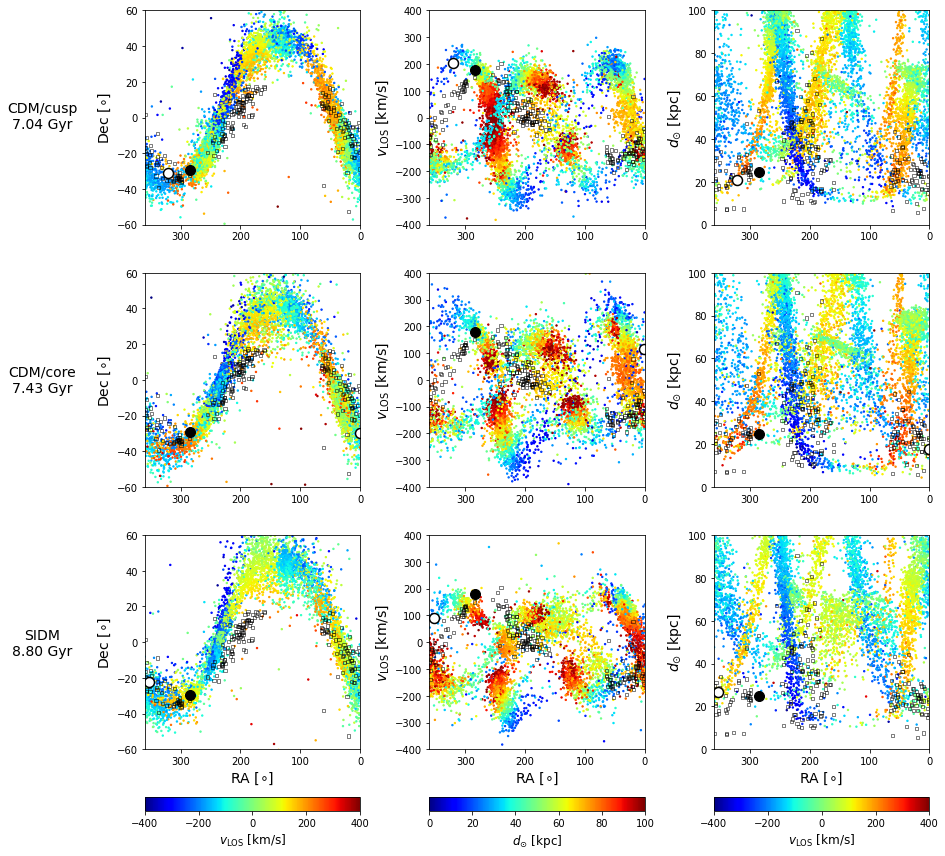
\includegraphics[width=1.0\linewidth]{figs/equatorial_2mass.png}
    \caption{%
        Right ascension, declination, heliocentric distance, and line-of-sight
        velocity for our simulated streams at their fifth pericenters. The white
        circle gives the position of the simulated progenitor; the black circle
        gives the observed coordinates of the progenitor.  The black squares
        correspond to 2MASS M-giant stars, identified by
        Majewski~\cite{majewski_two_2003}.
    }
    \label{fig:eq_2mass}
\end{figure}

This Figure appears to show good agreement especially between our CDM mergers
and the 2MASS data. In particular, the right ascension and declination data are
almost entirely reproduced by the CDM streams, with fairly good agreement in
terms of line-of-sight velocity and heliocentric distance. The SIDM stream,
however, gives a much poorer reproduction of the 2MASS stream. Most prominently,
at right ascensions near $200^\circ$, the corresponding declinations are all
significantly greater than the 2MASS data, exactly as was seen with the
\verb|SF| stream.

We next compare our data to specifically the heliocentric distances and
line-of-sight velocities by reproducing Figure~\ref{fig:vel_v_dist} with the
2MASS data overlaid. The result is shown in Figure~\ref{fig:vel_v_d_2mass}.
Again, we note that still-bound particles are colored black, and unbound
particles are colored according to the time when they came unbound.

\begin{figure}
    \centering
    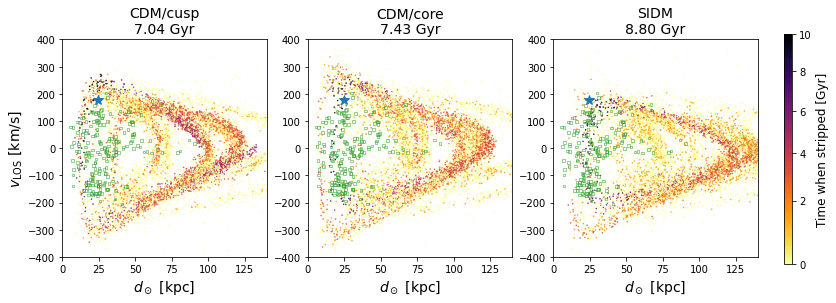
\includegraphics[width=1.0\linewidth]{figs/vel_v_dist_2mass.png}
    \caption{%
        Line-of-sight velocity versus heliocentric distance for each of the
        three mergers at their respective fifth pericenters with particles
        colored according to the time they came unbound (or black if they were
        still bound at the considered snapshot).  The blue star denotes the
        observed distance and velocity; the green squares denote data from
        2MASS M-giant stars.
    }
    \label{fig:vel_v_d_2mass}
\end{figure}

This Figure again shows good general agreement between the mergers and the
data.  In particular, the CDM/core merger accurately reproduces many of the
features of the 2MASS data at small heliocentric distances, including the
distances of the closest stars.  The CDM/cusp merger is the next most accurate
in this region, with its closest stars being only a small amount ($\sim 5$
kpc) farther away than given by 2MASS data.  The SIDM merger again has the
worst agreement of the mergers, with very few stars in the region of small
heliocentric distance and low line-of-sight velocity.

These plots give more evidence to believe that the distribution of
line-of-sight velocities in simulations of the Sgr stream can prove to show
important differences between the CDM and SIDM dark matter models. In
particular, our SIDM model appears to be significantly less able to accurately
reproduce the line-of-sight velocities of the Sgr progenitor and stream.

More generally, however, we find our CDM models are able to more faithfully
reproduce the observed qualities of Sgr than can our considered SIDM model.
To show that this trend holds more generally of dark matter self-interaction,
further studies are required.  We note in particular that we have considered a
rather large velocity-independent cross section ($\sigma/m = 10$ cm$^2$/g) and
have not varied the initial system parameters beyond what is done in the
Dierickx model.


% There also exist some differences between the three mergers in this frame.
% For example, the CDM/cusp run appears to have more particles with larger
% line-of-sight velocity magnitudes, with more stars that appear to be dark blue
% and red.  Inversely, the SIDM merger appears to have much more limited
% variation in line-of-sight velocity.  Also, the SIDM and CDM runs appear to
% have different features which are well-defined; the CDM runs show a rising
% stream arm at right ascension $\approx 350^\circ$ that is not well-represented
% in the SIDM run.  The SIDM run, however, has a more well-defined falling
% stream arm at right ascension $\approx 200^\circ$.

% To more fully explore these distances, we can look at histograms of the stellar
% particles' equatorial coordinates and proper motions and compare to the same for
% the \verb|STREAMFINDER| stars. We note, however, the presence of a very dense
% region of stars in the \verb|STREAMFINDER| data at $\text{RA} = 290^\circ$,
% $\text{Dec} = -30^\circ$, and $\text{dist} = 30$ kpc. This greatly skews the
% \verb|STREAMFINDER| distributions, so we cut it off in the plots in order to
% more fully elucidate the simulation distributions. The resulting histograms may
% be seen in Figure~\ref{fig:eq_hists}.

% \begin{figure}
%     \centering
%     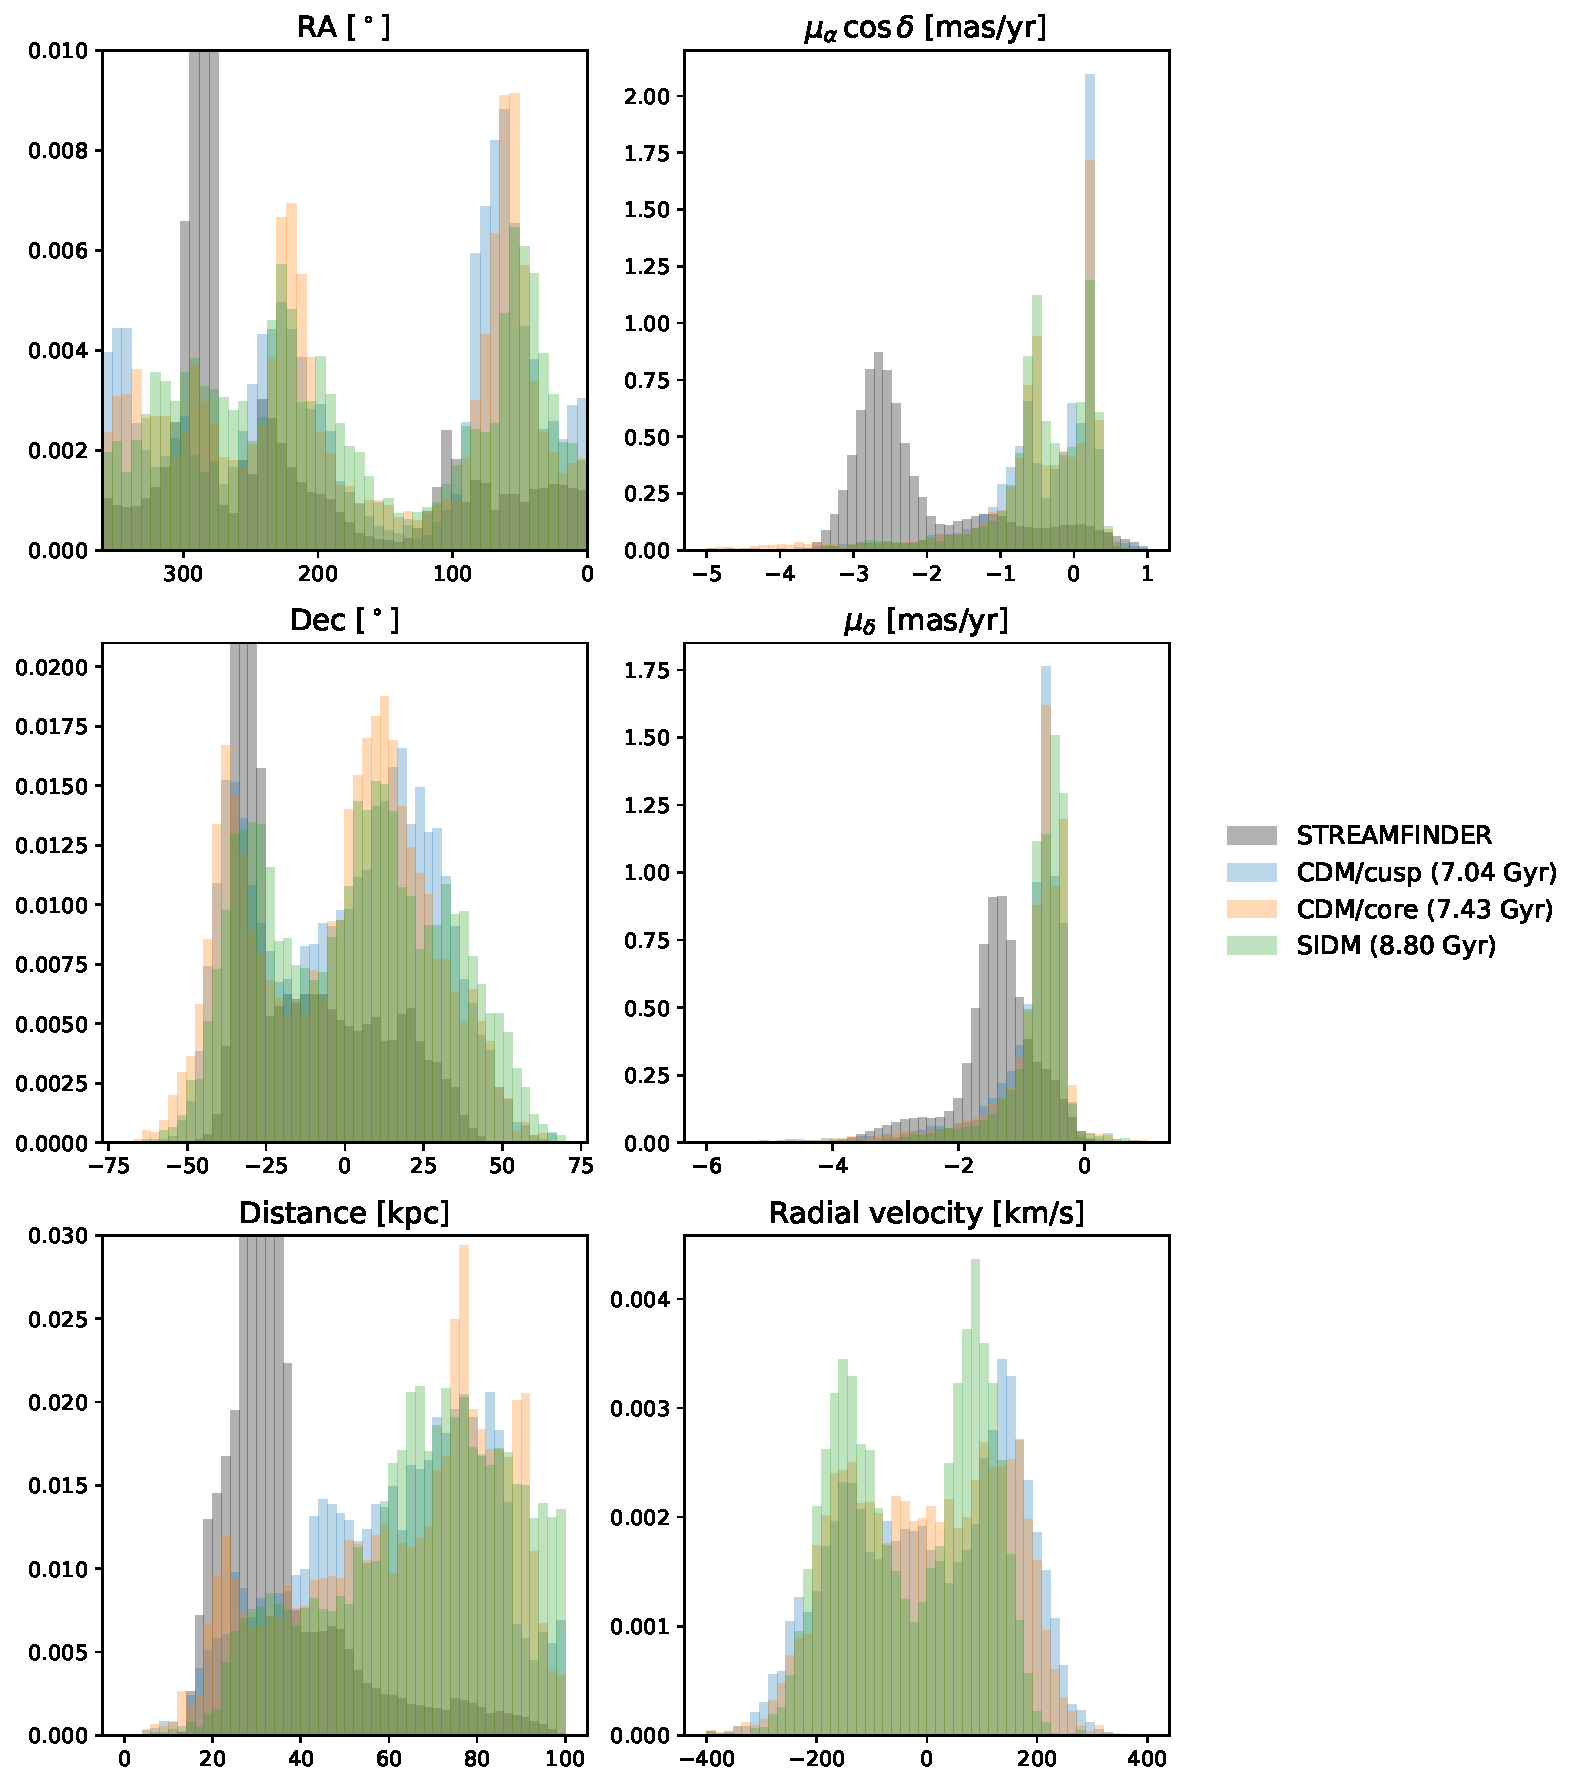
\includegraphics[width=0.9\linewidth]{figs/equatorial_hists.pdf}
%     \caption{%
%         Histograms of the equatorial coordinates and proper motions of the
%         simulated stellar particles closer than 100 kpc and the reference
%         \texttt{STREAMFINDER} stars (where possible).  Note that the
%         \texttt{STREAMFINDER} sample contains a very dense region which is
%         intentionally cut off in the right ascension, declination, and
%         distance plots in order to better see the simulated distributions.
%         All distributions are normalized to unity.
%     }
%     \label{fig:eq_hists}
% \end{figure}

% The histograms show us that the distributions of simulated stars are quite
% different than the \verb|STREAMFINDER| sample, particularly when we consider
% the proper motions and distances. Specifically, the $\mu_\alpha \cos\delta$
% distribution is largely concentrated between $-1$ and $0.5$ mas/yr for all
% three mergers, but appears to be a roughly unimodal distribution at $-2.5$
% mas/yr in the \verb|STREAMFINDER| data.  Similarly, all three mergers show a
% strong peak in $\mu_\delta$ at approximately $-0.5$ mas/yr, compared to the
% strong peak at $-1.5$ mas/yr in the \verb|STREAMFINDER| set. In the distance
% distribution, we see the distribution of distances appear to rise until around
% 60 to 80 kpc, compared to the sharp peak around 30 kpc in the
% \verb|STREAMFINDER| set with a decreasing frequency for larger distances.

% The declination plot shows the existence of peaks around $-30^\circ$ to
% $-40^\circ$ for all mergers and the \verb|STREAMFINDER| set. However, the
% mergers \textit{also} have a peak at around $+20^\circ$ that appears to be
% largely non-existent in \verb|STREAMFINDER|.  Lastly, we note that the right
% ascension plot shows some similarities between all mergers and the
% \verb|STREAMFINDER|: particularly, a peak at around $225^\circ$ and a trough
% at around $140^\circ$.

% The histograms also allow us to highlight some differences between the mergers
% themselves. In particular, the radial velocity histogram confirms the previously
% noted trend. The CDM/cusp merger appears to have more particles with higher
% radial velocity magnitudes than either of the other runs. The CDM/core merger
% appears to have a much flatter distribution of radial velocities than either of
% the other two mergers. The SIDM merger, on the other hand, has a strongly
% bimodal distribution of radial velocities, with strong peaks around $+100$ and
% $-150$ km/s.


\hypertarget{conclusions}{%
\chapter{Conclusions}\label{conclusions}}

% highlighting future to-dos and refinements, and identifying one or two key
% observations that should be pursued more carefully

In this work, we have presented a novel test of self-interacting dark matter
models by studying simulations of the infall of the Sagittarius dwarf
spheroidal galaxy.  Following the Dierickx 2017~\cite{dierickx_predicted_2017}
model, we have performed three simulations of the infall of Sgr.  Two of these
used the CDM model, one using initially cuspy halos and the other using cored
halos.  The third used the SIDM model, starting from cored halo profiles and
assuming a cross section of $\sigma/m = 10$ cm$^2$/g.

In our analysis of the resulting evolutions, we found that all three develop a
strong, streamlike shape.  The inclusion of self-interactions, however,
changes the shape dramatically, seemingly changing the overall rotation of the
outer stream arms and causing the loss of the intricate inner structure seen
in both CDM simulations.  In general, it appears that the SIDM simulation was
significantly more susceptible to the effects of tidal stripping.

Comparisons to existing Sgr data show generally good agreement especially with
our CDM streams.  For example, the stream shape seen in
\verb|STREAMFINDER| \cite{ibata_panoramic_2020} data is reproduced quite
faithfully in equatorial coordinates with similar distributions in
heliocentric distance.  Our mergers also show the predicted extension to the
stream introduced by the Dierickx 2017 model.  The SIDM stream, while
qualitatively similar to the \verb|STREAMFINDER| shape, shows the poorest
agreement of our three simulations with significantly larger declinations than
expected.  Similar findings were shown with a comparison to the right
ascension and declination data of M-giant stars from
2MASS~\cite{majewski_two_2003}.

Moreover, the resulting SIDM progenitor is much slower than either of the CDM
progenitors.  Its orbital time lags significantly, with the SIDM progenitor
reaching its fifth pericentric passage \textit{after} the cuspy CDM progenitor
is able to reach its sixth.  This, we believe, is intimately tied to
significantly smaller line-of-sight velocities at late times.  The SIDM
progenitor is in fact \textit{not} able to reproduce the observed heliocentric
distance and line-of-sight velocity of the Sgr progenitor at later times when
the stream is sufficiently developed in our simulation. Similarly, the SIDM
stream gives the least accurate reproduction of the heliocentric distance and
line-of-sight velocities of the 2MASS data.

These findings suggest that line-of-sight velocity in particular may serve as
an important discriminator for the existence of dark matter self-interaction.
However, there are many caveats with our findings that must be more thoroughly
examined in future studies. The first and most obvious is that we have only
considered a single, large, velocity-independent cross section of $\sigma / m =
10$ cm$^2$/g. Future studies should consider a wider range of cross sections, in
particular those close to 1 cm$^2$/g, and should consider adding
velocity-dependence to better match observational constraints. 

The next caveat is that we have only considered initial simulation parameters
(such as the initial position and velocity of Sgr) which were derived as
best-fit parameters for a CDM simulation. However, the optimal description of
the Sgr orbital history with SIDM likely differs from that of the CDM
description.  As such, the development of a semi-analytic model to explore a
wider range of parameters, as was done in~\cite{dierickx_predicted_2017}, would
help to identify such parameters and reduce any differences caused by this.

Future studies would also do well to improve the resolution of these
simulations.  Saving snapshots of the simulation at smaller time intervals
would significantly improve the ability to match the progenitor coordinates to
observation, which is currently time resolution-limited.  Using more stellar
particles would also likely improve the details in the resulting streams.  We
note further that the inclusion of a bulge in the galaxy profiles and the use
of other progenitor-identifying algorithms would be greatly helpful for more
accurately describing the trajectory of the simulated progenitors.

We note finally that the compilation of radial velocity data for more stars in
the Sgr stream would largely improve the comparisons we make with our mergers.
The \verb|STREAMFINDER| team note that nearly 3,000 stars in their stream have
radial velocity information in other public surveys; a compilation of these
data would help expand the comparisons that were made at the end of this work
and confirm whether the velocity distributions seen in our models are
observed.


% \printbibheading
\printbibliography

\end{document}